\chapter{Quantitative computerized analysis of idiopathic pulmonary fibrosis} \label{Yuwen_QuantitiativeAnalysis}

As introduced in Chapter 2, the natural history of IPF is poorly understood, and the clinical course for a given patient is unpredictable. Currently, there is a shortage of accepted bio-markers that can indicate the likely progression of IPF \citep{bartholmai2013quantitative}. A successful quantification scheme that allows for recognition of disease across radiology, pulmonary and pathology disciplines still remains difficult. Development of accurate and automatic tools for quantitative assessment of alterations in the lung with IPF will be essential for a rapid patient-specific diagnosis and treatment. To date, the shape of the lungs and lobes in IPF has not been quantified, and nor has the spatial distribution of tissue abnormalities. This chapter describes a study of quantitative analysis of IPF disease based on HRCT scans, including both assessment of tissue abnormalities and lung lobe shape analysis. 

\section{Background}
\subsection{Challenges of IPF diagnosis} \label{Challenge}
Managing patients with IPF presents a substantial health-care burden, due to short survival time and lack of effective treatments (with associated morbidity) \citep{olson2007mortality,raghunath2014quantitative}. Accurate assessment and diagnosis of IPF is very challenging, since there is significant individual radiological and physiological variability among patients \citep{devaraj2014imaging}. The progression of disease varies considerably, ranging from rapid worsening of symptoms to relatively slow deterioration over several years \citep{king2011idiopathic,richeldi2017idiopathic}. The American Thoracic Society (ATS) and European Respiratory Society (ERS) has developed a diagnostic criteria and schema for adult patients with IPF, and this criteria strongly recommends a multidisciplinary discussion between pulmonologists, radiologists and pathologists for an accurate diagnosis \citep{raghu2011official,travis2013official}. However, a successful classification and quantification tool that allows recognition of disease consistently across radiology, pulmonary and pathology disciplines still remains difficult. 

The complex appearances of IPF abnormalities that keep changing in extent over time is difficult to assess by traditional methods. Traditional radiological observation to distinguish disease patterns is tedious and not reproducible, and this manual evaluation is not consistent due to variation of inter- and intra- assessment \citep{flaherty2007idiopathic, watadani2013interobserver}. Specifically, the difference in perception and interpretation of visual features of disease, which is associated with the experience and skills of clinical doctors, may lead to variable description of the same patient or even cause ''reader error''. However, this ''error'' can not be fully solved by training or improvement of imaging technologies \citep{kundel2006history,bartholmai2013quantitative}. More importantly, the final decision of clinical diagnosis is often based on independent evaluation from the radiologist, clinician and pathologist, which makes it hard to ensure consistency and dependability of results  \citep{flaherty2004idiopathic,sverzellati2011method}. Another challenge of diagnosing IPF is the clinical problem of how to consistently detect and discriminate IPF from other idiopathic interstitial pneumonias (IIPs). These distinctive diseases usually have similar clinical presentations or indeterminate pathologic and radiographic appearances. Some cases may even have mixed restrictive/fibrotic and destructive/obstructive processes \citep{bartholmai2013quantitative}. For example, \gls{nsip}, a pathological subtype of IIPs, appears to behave similarly to those with IPF/UIP patterns, especially for the cases with coexisting UIP and fibrotic NSIP patterns \citep{monaghan2004prognostic, flaherty2001histopathologic}. All of these various IIPs have distinctly different prognosis, and specific therapy that is targeted to a particular pathological process is becoming necessary \citep{lynch2005high}. Therefore, non-IPF IIPs must be discriminated from IPF \citep{bjoraker1998prognostic}. 

\subsection{Advantages of quantitative analysis using HRCT} \label{Advantages}

Recent development in radiological imaging techniques offers exciting opportunities to develop radiological patient-specific biomarkers as important indicators of specific phenotypes \citep{devaraj2014imaging,gotway2007challenges}. HRCT has played an essential role in evaluating lung disease through recognizing visual patterns and features of disease regions such as ground-glass opacities, reticular patterns and honeycombing \citep{mueller2007every}. HRCT is also a useful diagnostic tool to differentiate between IPF and other pathologies. It is generally believed that the extent of visual lesion present on HRCT strongly relates to the severity of pathological abnormalities, and therefore can be used to monitor the progression of disease and then response to therapy \citep{kazerooni1997thin,kim1999nonspecific,wells2003idiopathic,saketkoo2011developing}. In addition, it has been noted that the use of HRCT can actually decrease the need for surgical lung biopsy which is risky for older patients with comorbidities \citep{bartholmai2013quantitative}. As a non-invasive tool for visualizing abnormal parenchymal densities, HRCT has its own advantage in IPF diagnosis even for the cases where HRCT fails to show enough specific features to reflect typical UIP pattern, since HRCT can provide guidance for optimizing the site to obtain a surgical lung biopsy \citep{kazerooni2001high, diette2005high, misumi2006idiopathic, costabel2007diffuse}. 

Currently, how the changes of disease can be consistently characterized and quantified over time and how these changes can predict disease progression are still challenging tasks. Manual classification and subjective evaluation are usually complicated and not accurate enough. Image-based quantitative analysis is therefore strongly needed for developing a robust and consistent IPF assessment system \citep{gotway2007challenges,lynch2005high}. A number of studies have indicated that the quantification of abnormalities on thoracic HRCT has potential to determine the extent of disease. Moreover, it can help with stratifying different types of disease with numerous imaging features in variable distribution \citep{best2008idiopathic,wells2003idiopathic, sumikawa2008computed, bartholmai2013quantitative}. The hypothesis is that through quantifying abnormalities from radiological images, robust objective bio-markers can be developed to drive a patient-specific prediction based on specific phenotypes. This will be important for facilitating individualized clinical management and identifying specific phenotypes linked to clinical disease presentations or therapeutic responses \citep{raghunath2014quantitative}.
\newpage

\subsection{Review of current published methods of quantitative analysis of lung disease} \label{Review}
In the past few years, there has been considerable effort to provide quantitative analysis of lung parenchymal abnormalities on HRCT scans. Fortunately, quantitative methods to analyse disease patterns of \gls{copd} such as emphysema have been well developed over the last 20 years, and have been able to provide reproducible bio-markers used in sub-clinical diagnosis and assessment \citep{da2008identification,gietema2011quantifying,galban2012computed,wang2013high,castaldi2013distinct}. However, quantification of disease patterns of lung fibrosis or other interstitial lung disease is more challenging, since the appearances and changes of these abnormalities are even more complicated than the characteristics seen with emphysema \citep{lynch2007quantitative, delorme1997usual, galban2012computed, depeursinge2010comparative}. In the early days, first-order textural analysis methods such as \gls{mld} and histogram analysis (HIST) were used to analyse radiological lung imaging \citep{gilman1983ct,gould1988ct,muller1988density,kinsella1990quantitation,knudson1991expiratory,behr1992evaluation}. These approaches to assess CT data are automatic and objective, but they simply examined a single parameter for the whole lung. The measurement of attenuation (which relates to density) is highly dependent upon lung volume and can be significantly affected by beam-hardening effects, scatter and drifts in scanner calibration. Therefore, these methods are difficult to apply in the presence of mixed disease.

\cite{uppaluri1999interstitial,uppaluri1999computer} was an early group to present a multiple feature based method to automatically quantify and classify pulmonary parenchyma of interstitial lung disease based upon HRCT. An adaptive multiple feature method (AMFM) which combined statistical texture measures with a fractal measure was developed to initially assess the emphysema regions of the lung, and subsequently extended to study subjects with IPF or sarcoidosis. AMFM was further improved to assess as many as 22 independent texture features which enabled classification of pulmonary parenchymas into six tissue patterns, including: honeycombing, ground-glass, broncho-vascular, nodular, emphysema-like, and normal. These 22 texture features consist of statistical features (grey level distribution features, run-length features and co-occurrence matrix features) and fractal features (geometric fractal dimension and stochastic fractal dimension). The lung slices were divided regionally into $31 \times 31$ pixel regions of interest (ROI). In each ROI, an optimal subset of texture features was evaluated to determine which of the six patterns in the region could be characterized. A non-linear statistical classifier, the Bayesian classifier, was built to do the classification through calculating the probability that the ROI belongs to each tissue pattern. The whole algorithm contains two stages: the first stage involves training AMFM to recognize different HRCT based tissue patterns using a preselected dataset; the second stage involves a new CT data to be analysed using the above introduced method. This multiple textural feature based method established the foundation and framework for subsequent studies on quantitative assessment of lung imaging. \cite{xu2006computer,xu2006mdct} enhanced the ability of AMFM based on the work of \cite{uppaluri1999interstitial,uppaluri1999computer}. In this study, the 2D textural feature-based tissue analysis method was extended to 3D space for quantifying emphysema and early smoking related lung pathologies. The extracted features involved both first-order features (mean, variance, kurtosis and entropy of grey level distribution) and second-order features (run-length and co-occurrence measurements). The results showed that 3D AMFM analysis of lung parenchyma improved discrimination compared to 2D AMFM of the same volumes of interest (VOIs). 

In the past 15 years, AMFM has been widely used to quantify and classify lung disease from CT imaging \citep{van2002automatic,chabat2003obstructive,best2003quantitative,uchiyama2003quantitative,kim2005computer,zavaletta2006high,arzhaeva2007computer,best2008idiopathic,kim2010computer,kim2011quantitative,kim2015comparison}. A general workflow of texture analysis is: 1. preset several types of tissue patterns; 2. divide lung slices into a set of ROIs with a square shape; 3. use texture analysis to extract multiple features for each ROI; 4. select representative expert-labelled ROIs as a training set for a classifier; 5. use the features of ROIs from a new set as input to the classifier to find the corresponding tissue pattern. Currently, most of the published CT based lung tissue analysis methods were developed based on this framework. Different textural features, ROI sizes or classifier types were specifically selected to target different lung disease or clinical requirement. \cite{best2003quantitative,best2008idiopathic} used mean lung attenuation (MLA), skewness (asymmetry) and kurtosis (peakedness) as features combined with a further univariate and multiple correlation and regression statistical analysis to determine relationships between histogram signals and results of PFTs in patients with IPF. The result showed that CT histograms of the lungs were correlated with PFT measurements, therefore the visual disease extent on CT images can be used as a strong independent predictor of mortality in IPF. \cite{chabat2003obstructive} used similar textural features and classifier to the method of \cite{best2003quantitative,best2008idiopathic} for differentiating centrilobular emphysema, panlobular emphysema, constrictive obliterative bronchiolitis and normal lung tissue. \cite{zavaletta2007high} trained and tested three classifiers which included 10 Nearest Neighbour Classifier, Fisher Linear Discriminant Analysis, and Parzen Window to classify normal and abnormal structures in lungs with IPF. 

\cite{uchiyama2003quantitative} and \cite{kim2005computer} employed multi-layered \gls{anns} with a back-propagation algorithm as a classifier to distinguish between different tissue patterns which includes both normal and diffuse lung disease slices. ANNs, using their simplest definition, are the modelling of the human brain, and their building blocks are neurons. They are excellent tools for finding patterns which are too complex or numerous for a human programmer to extract and teach the classifier to recognize, therefore will increase the accuracy of classification. In addition, \cite{kim2010computer,kim2011quantitative,kim2015comparison} published a series of papers presenting a texture-based computer-aided diagnosis (CAD) scoring system to assess \gls{qlf} as a measurement of lung disease severity and as a surrogate imaging marker. The QLF score (a texture feature-based measure) was compared to the CT histogram metric (a global statistical measure), and the baseline severity and early change within 7 months in patients with IPF was assessed. The result concluded that classifier-model-derived scores (QLF scores) were associated with baseline disease extent and were also a sensitive measure of change over time, and a QLF score could be used for measuring the extent of disease severity and longitudinal changes.

Most published methods focus on texture-based classification of lung parenchyma or the severity and volumetric quantification of disease for the whole lung (such as the QLF score). Currently, very few studies attempt to quantitatively characterize the spatial distribution of each disease pattern or describe how each tissue pattern changes or converts over time. Moreover, many of the existing methods are time consuming and sometimes even require several hours. These real-world limitations present difficulties when translating these techniques into clinical applications \citep{bartholmai2013quantitative}.

In addition, it has been generally believed that there is a decrease in lung volume (both FRC and TLC) in patients with IPF, but up to now, few studies have been presented to explore the lung and lobe shape alteration in IPF lungs compared to normal ones. It is a reasonable assumption that shape changes will be observed in IPF lungs due to physiologic alterations and disease progression over time. 

\subsection{Computer-Aided Lung Informatics for Pathology Evaluation and Ratings} \label{CALIPERIntroduction}
CALIPER (Computer-Aided Lung Informatics for Pathology Evaluation and Ratings) is a computational image analysis platform developed by the Biomedical Imaging Resource Laboratory at the Mayo Clinic (Rochester, MN, USA) for the characterization and classification of lung parenchymal findings on HRCT \citep{maldonado2013automated,bartholmai2013quantitative,raghunath2014quantitative}. The data processing step includes lung segmentation and classification of the remaining pulmonary parenchyma on the CT dataset. Briefly, CALIPER isolates the lung parenchyma by extracting central airways and vascular structures, and then classifies every parenchymal voxel into the following characteristic CT patterns: normal (N), reticular (R), honeycomb (HC), ground-glass (GG), mild \gls{laa}, moderate LAA, and severe LAA (including emphysema). This novel computer-aided method for analysing pulmonary tissue features provides a consistent and reproducible quantification of lung disease that relates to the semi-quantitative assessment from radiologists\citep{maldonado2013automated}. Figure \ref{fig:CALIPERPatterns} shows visual appearance of each characteristic CT pattern.

\begin{figure*}[htbp]
  \centering 
  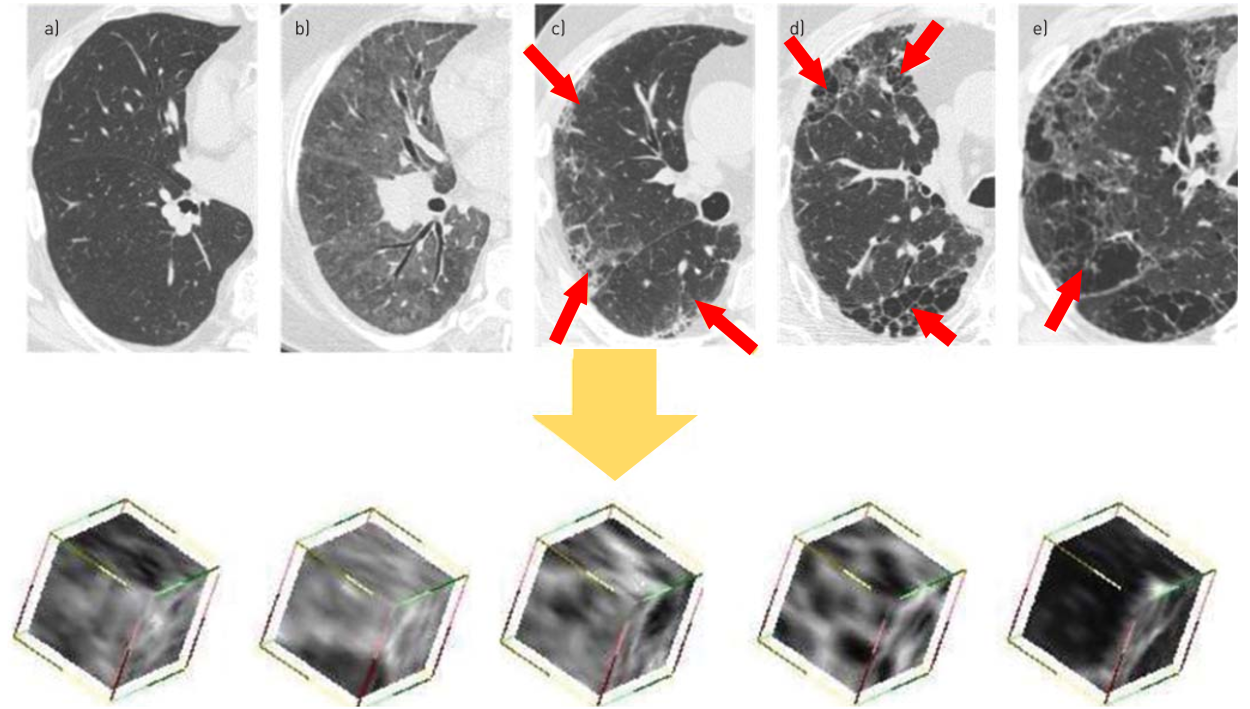
\includegraphics[height=3.0in]{QuantitativeAnalysis/Image/CALIPERPatterns.png}
  \caption{Computed tomography images demonstrating appearance and various visual manifestations of idiopathic pulmonary fibrosis: a) normal, b) ground glass, c) reticular changes (arrows), d) honeycombing (arrows) and e) emphysema (arrow). In training datasets, the consensus of four thoracic radiologists was used to identify multiple volumes of interest (VOIs) corresponding to normal, ground-glass density, reticular abnormalities, honeycombing and emphysema. Reproduced from \citep{maldonado2013automated}.}
  \label{fig:CALIPERPatterns}
\end{figure*}

Pre-processing is conducted before the eventual classification of the pulmonary parenchyma. This requires segmentation of anatomic lung regions. The lungs are initially segmented using an adaptive density-based morphology (thresholding) method \citep{hu2001automatic}. Airways are segmented by thresholding combined with a 3D region growing algorithm and vessels are segmented by an enhancement filter based on Hessian matrix \citep{sato2000tissue}, then the final lung segments are extracted. 

The volumetric detection and classification of pulmonary parenchyma by CALIPER uses a sliding window supervised classification scheme based on histogram signature mapping techniques \citep{zavaletta2007high}. This classification technique was trained by expert radiologists via consensus assessment of pathologically confirmed datasets, which were obtained from the Lung Tissue Research Consortium (LTRC). LTRC is a resource program sponsored by the NIH/NHLBI that provides clinical and physiologic data of human lung tissues to qualified investigators for use in their research and to help investigators develop a better understanding of lung disease. The central part of the classification scheme is the selection of a set of expert-labelled \gls{vois} as the training data for a classifier. The training data used in CALIPER comprises $15 \times 15 \times 15$-voxel VOIs acquired from HRCT scans of subjects with proven pathological diagnosis of interstitial lung disease (ILD) or emphysema from the LTRC repository. These VOIs were selected from CT scans through independent analysis by four experienced thoracic radiologists, with instructions and criterion to determine if the visual appearance should represent normal, emphysema or one of the characteristic lung fibrosis CT patterns: honeycomb, reticular or ground-glass \citep{maldonado2013automated,bartholmai2013quantitative}.

The VOIs with agreement by all four radiologists on the class of abnormality were used as exemplars to determine canonical histogram signatures of the CT patterns of visual abnormality by automatic cluster affinity techniques. Quantitative discriminability of a series of pairwise dissimilarity metrics based on the VOI histograms was tested using \gls{mds}. The \gls{cvm}, which was found to be most the consistent with the expert groupings, was selected as the dissimilarity metric to train CALIPER. For each of the parenchymal voxels needing to be classified, the local histograms of its neighbouring $15 \times 15 \times 15$ voxels were compared against the histograms of the exemplars identified in the training phase. A CVM dissimilarity measure was used in the comparison and the fundamental type of the exemplar (N,R,H,G or emphysema) with the lowest CVM was assigned as the parenchymal CT pattern to this classified voxel. The parenchymal voxels identified as vessel structures were classified as normal pattern. Figure \ref{fig:CALIPERResults} shows a representative dataset with axial, coronal and sagittal sections of a CT lung volume where every voxel of the parenchyma is characterized and colour coded into one of the parenchymal patterns (N, R, H, G, and mild, moderate and severe LAA). 

\begin{figure*}[htbp]
  \centering 
  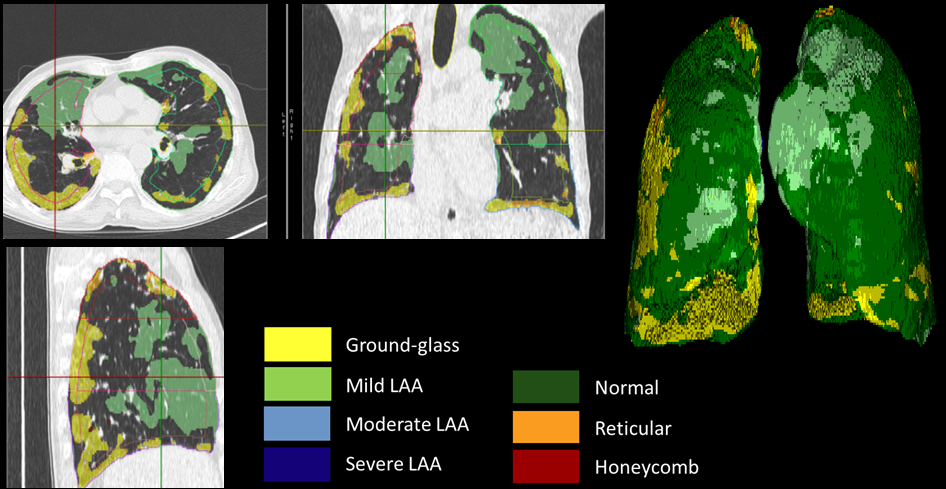
\includegraphics[height=2.9in]{QuantitativeAnalysis/Image/CALIPERResults.png}
  \caption{Color labelled classification result from CALIPER of one subject diagnosed with IPF.  (a) Transverse plane. (b) Coronal plane. (c) Sagittal plane. (d) 3D color labelled lung.}
  \label{fig:CALIPERResults}
\end{figure*}


%%%%%%%%%%%%%%%%%%%%%%%%%%%%%%%%%%%%%%%%%%%%%%%%%%%%%%%%%%%%%%%%%%%%%%5
\section{Methods: quantitative analysis of IPF lungs}
This section describes the quantitative methods used in this chapter to analyse and characterize IPF tissue abnormalities and lung lobe shape, longitudinally and in comparison to normal subjects. In summary, HRCT imaging was classified by pattern using a validated image analysis process (CALIPER) \citep{maldonado2013automated,bartholmai2013quantitative,raghunath2014quantitative}. The tissue classification data was mapped to a mean statistical shape model (SSM) allowing a quantitative approach to analyse tissue pattern density, tissue pattern volume, spatial distribution of abnormalities, and regional changes in tissue abnormalities over time. In the shape analysis, lobar finite element meshes for both IPF and normal subjects were projected to the SSM, and lobe shape differences in IPF were then quantitatively characterized.

%%%%%%%%%%%%%%%%%%%%%%%%%%%%%%%%%%
\subsection{Tissue classification of IPF lungs}
\subsubsection{Imaging and clinical data}
Data used in this study was acquired as part of routine clinical diagnosis or follow up. Data use was approved by the Southern Health and Disability Ethics Committee. Data include volumetric HRCT and PFTs from 13 patients who were diagnosed with or suspected to have IPF. All patients were under clinical care at Auckland City Hospital, Auckland, New Zealand. Volumetric HRCT images (slice thickness 1.25-5.00 mm) were acquired at the end of inspiration during routine diagnostic inspection and/or monitoring for IPF disease. Eleven of the subjects had more than one serial CT scan within a 5-79 month interval, representing different time points (7 subjects had 3 time points, 4 subjects had 2 time points). The population demographics for these subjects is shown in Table \ref{tab:DemographicData}.
\newpage

\begin{table}[h]
\centering
\caption{Demographic data.}
\label{tab:DemographicData}
\begin{tabular}{| l  | c | c|}
\hline
{\bf Description}  \\ \hline
Age (years) & 43-83 \\
\hline
Females/Males	& 3/10 \\
\hline
Slice thickness	& 1.25-5.00 mm \\
\hline
Scan month interval	& 5-79 month \\
\hline
Slice resolution	& 512 $\times$ 512 mm \\
\hline
Number of slices	& 68-227
\\ \hline
\end{tabular}
\end{table}

%%%%%%%%%%%%%%%%%%%%%%%%%%%%%%%%%%
\subsubsection{Normalization of classified data} \label{DataNormalization}
Tissue CT patterns for each patient at each time point were classified using the CALIPER software introduced in Section \ref{CALIPERIntroduction}. Then, lung surface data and fissure surface data were acquired using the lobe segmentation method introduced in Chapter 3. A bi-cubic Hermite finite element surface mesh was fitted to the shape of the lung and its fissures via a least squares fit using the CMISS software package (https://www.cmiss.org). The details for the generation of lobe data and the lobe mesh are given in Chapter 3, Section \ref{ShapeModelGeneration}.

There is lung shape variation between different subjects and often between clinical images obtained at different times, as well as variation in the extent to which a patient inhales during imaging, even with careful training. Thus, the classified volumetric lung data was then mapped to a statistical shape model (SSM) of the ''normal'' older human lung to provide a consistent mapping of tissue abnormalities in individuals to a consistent lung shape. The steps for the construction of the SSM were introduced in Chapter 3, Section \ref{ShapeModelGeneration}, which described an SSM for a cohort aged 21-83. In this chapter, data from 35 normal subjects aged 50 years and older were used to derive an SSM because this is consistent with the typical age of onset of IPF. The SSM used for mapping data is the average mesh of the lung lobes which was derived from these 35 training subjects, and it provides a description of a statistical mean lung and fissure surface shape for a cohort of normal adults aged $>$ 50 years.

In order to map the individual classified data to the SSM mesh, the bi-cubic Hermite finite element mesh of the lung surface was converted to a tri-cubic Hermite volumetric mesh which describes not only the lung surface but also the internal anatomy \citep{tawhai2003developing}. The volumetric mesh has 40 nodes and 30 elements for left lung, and 56 nodes and 38 elements for right lung. Each node has 24 DOFs which store the global coordinates (x, y and z) and the first, second and third nodal derivatives (\pd{n}{\xi_1}, \pd{n}{\xi_2}, \pd{n}{\xi_3}, \pd[2]{n}{\xi_1 \xi_2}, \pd[2]{n}{\xi_2 \xi_3}, \pd[2]{n}{\xi_1 \xi_3} and \pd[3]{n}{\xi_1 \xi_2 \xi_3}), where n is x, y and z, and $\xi$ is the local element coordinate.

During the data mapping, all of the classified data should be completely enclosed inside its lobe volume mesh. The position of each point within the finite element mesh was defined locally in each element of the mesh by $\xi_{i}$, for i=1,..,3 with $0<\xi_{i}<1$. The $\xi_{i}$ location denotes the local coordinates of the data point with respect to its element. The local coordinate $\xi_{i}$ was then used to calculate the global coordinates of the mapped data points using

\begin{equation}
u(\xi_{i}) = \sum_{n=1}^{N} \psi_n(\xi_{i})u_n,
\end{equation}
where $u_n$ is a vector of N element nodal parameters of the SSM lobe mesh associated with the interpolation functions $\psi_{n}$. 

In order to force a uniform data point distribution throughout each lung, the gaps in the mapped data caused by the mapping deformation from individual shape to SSM (shown in Figure \ref{fig:GapFilling-a}) were ''filled'' by matching the classification of their closest neighbour point among the classified data. Uniform data point distribution facilitates further density and spatial distribution analysis of abnormalities. Briefly, the gaps in the mapped data were filled using the following steps: 

1. Mapped data were cut into a series of axial slices (shown in Figure \ref{fig:GapFilling-a}).

2. The lung mesh of average SSM was used as a mask to define the lung boundary. (shown in Figure \ref{fig:GapFilling-b}).

3. Morphological operations were applied to smooth the lung boundary, then a lung mask was generated (shown in Figure \ref{fig:GapFilling-c}).

4. The gaps enclosed inside the lung mask were filled with the CT pattern color of its closest point among the classified data (shown in Figure \ref{fig:GapFilling-d}).

\begin{figure*}[htbp] 
\centering
\begin{subfigure}{.28\linewidth}% set image scale
  \sbox0{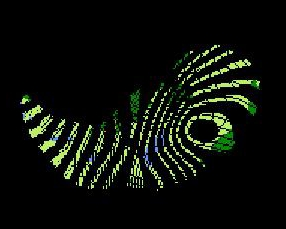
\includegraphics{QuantitativeAnalysis/Image/GapFilling1.jpg}} 
  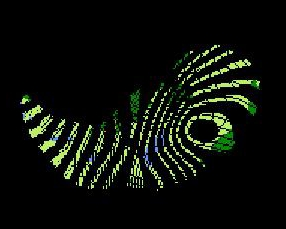
\includegraphics[width=\linewidth,trim={{.0\wd0} {.0\wd0} {.0\wd0} {.0\wd0}},clip]{QuantitativeAnalysis/Image/GapFilling1.jpg} %trim={<left> <lower> <right> <upper>}, set the cut scale
  \caption{Axial slices with gaps\\ \quad}
  \label{fig:GapFilling-a} 
\end{subfigure} 
%\vspace{.3in} % control space between the upper context and figure
\hspace{.5in} % control space between two figures
\begin{subfigure}{.28\linewidth}% set image scale
  \sbox0{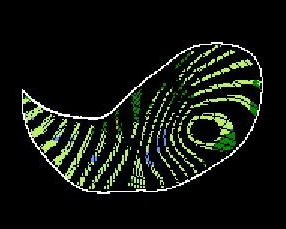
\includegraphics{QuantitativeAnalysis/Image/GapFilling2.jpg}}
  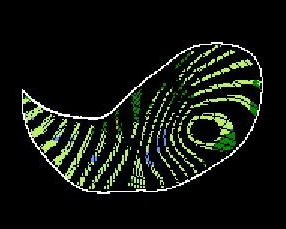
\includegraphics[width=\linewidth,trim={{.0\wd0} {.0\wd0} {.0\wd0} {.0\wd0}},clip]{QuantitativeAnalysis/Image/GapFilling2.jpg}
  \caption{Lung boundary\\ \quad}
  \label{fig:GapFilling-b} 
\end{subfigure}
\hspace{.5in}
\begin{subfigure}{.28\linewidth}% set image scale
  \sbox0{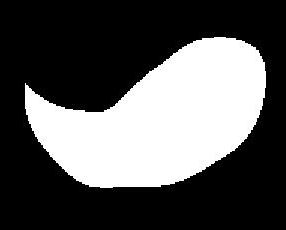
\includegraphics{QuantitativeAnalysis/Image/GapFilling3.jpg}}
  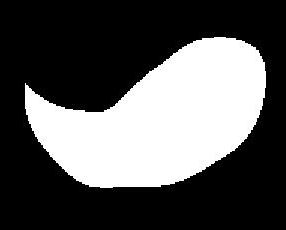
\includegraphics[width=\linewidth,trim={{.0\wd0} {.0\wd0} {.0\wd0} {.0\wd0}},clip]{QuantitativeAnalysis/Image/GapFilling3.jpg}
  \caption{Lung mask}
  \label{fig:GapFilling-c} 
\end{subfigure}
%\vspace{.3in} % control space between the upper context and figure
\hspace{.5in} % control space between two figures
\begin{subfigure}{.28\linewidth}% set image scale
  \sbox0{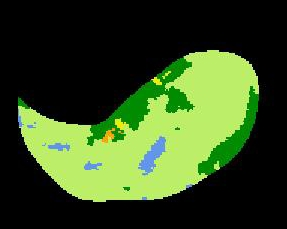
\includegraphics{QuantitativeAnalysis/Image/GapFilling4.jpg}}
  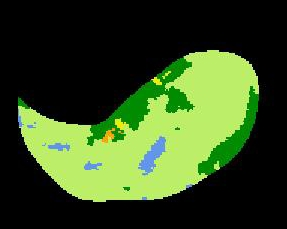
\includegraphics[width=\linewidth,trim={{.0\wd0} {.0\wd0} {.0\wd0} {.0\wd0}},clip]{QuantitativeAnalysis/Image/GapFilling4.jpg}
  \caption{Gap filled slice}
  \label{fig:GapFilling-d} 
\end{subfigure}
\caption{Diagram of gap filling steps within the mapped data. (a) Get axial slices of mapped data (with gaps). (b) Define lung boundary (SSM defined). (c) Get lung mask. (d) Fill the gaps within lung mask.}
\label{fig:GapFilling}
\end{figure*}

%%%%%%%%%%%%%%%%%%%%%%%%%%%%%%%%%%
\subsection{Tissue quantification of IPF lungs} \label{TissueQuantification}
\subsubsection{Density analysis}
The average density value of each classified CT pattern was calculated. In a typical CT image, intensity is measured in Hounsfield units (HU) which corresponds linearly to the actual density of the imaged tissue. HU was calculated with the segmentation software PTK calibrated to values of -1024 for air density, zero for water density, and over 40 for blood, bone, and other non-parenchymal tissue. The tissue density ($\rho$, $g/cm^3$ ) was then acquired at each voxel using

\begin{equation}
\rho = \frac{HU}{1024} + 1.
\end{equation}

The average density of each CT pattern was then calculated from individual voxel density.

\subsubsection{Spatial distribution analysis}
Based on the criteria of IPF defined by the ATS and ERS, the diagnosis of IPF is usually associated with the presence of a UIP pattern in HRCT (see details in Chapter 2, Section \ref{DiagnosisCriteria}). The distribution of UIP on HRCT is characteristically basal and peripheral (subpleural), though often patchy. Therefore, in order to quantitatively analyse the spatial distribution of IPF abnormalities, the percentage of honeycomb, reticular, emphysema and ground-glass which represent typical UIP disease patterns on HRCT were calculated in basal-to apical sections, dorso-to-ventral sections, from subpleural to internal, and by lobe: 
\newpage

\paragraph{Basal-to-apical:} In the direction from base to apex, the volume percentage of each disease region was averaged in bins representing 5\% of lung height (along the cranio-caudal axis). 

\paragraph{Dorso-to-ventral:} In the direction from posterior to anterior, the volume percentage of each disease region was averaged in bins representing 5\% of distance along the cranio-caudal axis. 

\paragraph{Subpleural to internal:} The distance from the abnormalities to the boundary of the lung and to the centre of the lung were measured to analyse the location of disease with respect to the lung surface. To be specific, the centre location of each connected cluster of disease area was firstly extracted, and the subpleural to internal distance percentage $R_{subpleural}$ of each connected cluster, which described how far the connected cluster was from the lung surface, was then calculated as in Figure \ref{fig:SubpleuralMethod}.

\begin{figure}[H]
  \centering 
  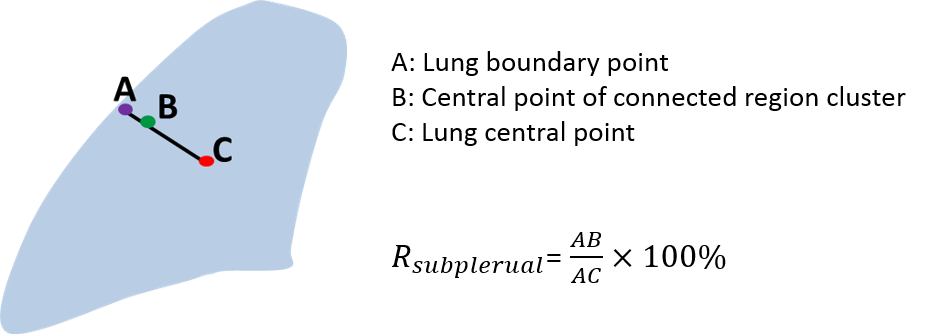
\includegraphics[height=1.8in]{QuantitativeAnalysis/Image/SubplesrualMethod.png}
  \caption{Diagram of subpleural-to-internal percentage measurement.}
  \label{fig:SubpleuralMethod}
\end{figure}
%
%\begin{equation}
%R_{subpleural} = \frac{AB}{AC} \times 100
%\end{equation}

The coordinate of the lung central point $P_{centre}(x,y,z)$ was calculated as

\begin{equation}
P_{centre}(x,y,z) = \frac{\sum\nolimits_{i=1}^N P_{surface}(x,y,z)}{N},
\end{equation}

\noindent where $P_{surface}(x,y,z)$ is the coordinate of the lung surface data point, and N is the number of lung surface data points.

\paragraph{Lobar distribution:} In order to analyse the lobar distribution of disease, the volume percentage of each disease CT pattern located in each lobe was calculated.

\subsubsection{Change in classification of tissue pattern over time}
Median survival time of patients with IPF is generally from 3 to 5 years from time of diagnosis. However, individual progression of disease is variable and how the characteristic disease pattern changes over time (e.g. whether a disease region deteriorates and changes to other tissue patterns or stays the same over time) still remains elusive. In this study, the classified data of all subjects and time points have been normalized to a standard lung shape (SSM, as introduced in Section \ref{DataNormalization}), thus making it possible to detect the disease change in specific regions over time, by extracting the CT pattern of each voxel at different time points.

\subsection{Volume analysis of IPF lungs} \label{VolumeAnalysis}
\subsubsection{The change of whole lung volume over time}
The volume of each classified tissue pattern in both left and right lung was calculated using the following equation:

\begin{equation}
V_{Region} = N \times R_x \times R_y \times R_z
\end{equation}

\noindent where N is the number of voxels of each tissue pattern, $R_{x}$, $R_{y}$ are the x, y resolution of the CT scan, and $R_{z}$ is the thickness of the CT scan. Then the whole volume of left and right lung was calculated as the sum of the volume of each CT pattern.

%\subsubsection{The change of tissue volume over time}
%Currently, there is little research on investigating the volume change of individual tissue classifications over time. In Section \ref{TissueQuantification}, it was demonstrated that the distribution of tissue abnormalities changes as time goes on. In this section, the volume percentages of normal tissue and classified fibrosis tissue (honeycomb, reticular and ground-glass) in left and right lung for each time point were calculated to analyze the change of tissue volume over time.

\subsubsection{Lobe volume difference between old normal lungs and IPF lungs}
The lobe volume of the IPF cohort was compared with the older normal cohort described in Section \ref{DataNormalization}. In order to quantitatively analyse the lobe volume difference between the two groups, the volume proportion of each lobe was calculated as:

\begin{equation}
 \label{eq:FissurePrediction1}
 P_{i} = \frac{V_{i}}{\sum_{i=1}^{5}V_i},
\end{equation}

\noindent where $V_{i}$ is the volume of each lobe with i=1 corresponding to left lower lobe, i=2 corresponding to left upper lobe, i=3 corresponding to right lower lobe, i=4 corresponding to right middle lobe and i=5 corresponding to right upper lobe. The differences in lobe volume proportions between IPF subjects and normal subjects were compared statistically using a t-test. In order to further compare lobe volumes between these two groups, the average lobe volume proportion among IPF subjects and among the normal subjects were then calculated.

\subsection{SSM based shape analysis of IPF lungs} \label{SSMBasedAnalysis}
The SSM was used to quantitatively analyse the alterations in lung lobe shapes of patients with IPF. As previously described in Section \ref{DataNormalization}, 35 normal subjects aged $>$ 50 years were used as training data to construct the SSM which contained both lung surface and fissure surface. PCA was used to decompose the shape variation of the lung lobe into a set of modes, and each mode represented one type of lung and fissure surface shape variation. Thus, each lung lobe shape was described by a linear combination of the mode vector and its corresponding weight by

\begin{equation}
 \label{eq:FissurePrediction1}
 S_{new} = S_{mean} + \sum_{i=1}^L \mathbf{u}_i w_{i},
\end{equation}

\noindent where $S_{mean}$ is the average lobe shape model across all the training subjects, $\mathbf{u}_i (i = 1,2...L, L=34$ in this study) is the mode vector of shape variation which corresponds to the $i^{th}$ largest principal component from PCA, and $w_{i}$ is a weight factor given to each mode of variation. 

The lung lobe FE mesh of each IPF subject was then procrustes projected on to the average SSM after alignment to the reference model (details can be seen in Chapter 3, Section \ref{MeshPrediction}) The new weight values of all shape modes $w_{new} = [w_{new1}, w_{new2},...,w_{newL}]$ (L = 35) were calculated from the projection. These mode weights can be used as quantitative indexes to analyze and compare the shape variation and difference between IPF and the control group.

\subsubsection{Shape difference between IPF lungs and normal control lungs}

For the SSM of the control group, the first three shape modes explained over 30\% of the total variation in the training set. Therefore, the weight values of the first three modes were used as the measurement to compare the shape difference of lung lobe between controls and IPF. The p-values of the first three shape modes between the two groups were calculated using a t-test.

\subsubsection{Relationship between lung lobe shape and fibrosis and low attenuation area extent}
In order to quantitatively investigate the association between fibrosis extent and lung shape variation, the association of the first three mode weightings with the overall volume percentage of fibrosis and low attenuation area (LAA) was estimated using linear regression. Total fibrosis extent was estimated as the sum of reticular, honeycomb and ground-glass opacification of both lungs, and total LAA extent was estimated as the sum of mildLAA,  moderateLAA and severeLAA of both lungs. The behaviour of the first three modes with respect to overall fibrosis percentage and LAA percentage was analysed using linear regression.

\section{Results}
\subsection{Normalization of classified data}
The data classified using the CALIPER software were mapped to the SSM using the method introduced in \ref{DataNormalization}. Figure \ref{fig:MainMappingResult} shows the mapped classification data for a single subject. The mapped data for the other subjects can be found in Appendix \ref{MappedClassificationData}.

\newgeometry{bottom=4cm} %set the left margin of page
\begin{landscape}
\begin{figure}[htbp]
\begin{subfigure}{6.5cm}
    \makebox[60pt]{\raisebox{50pt}{\rotatebox[origin=c]{0}{\minibox{Classified\\ data}}}}%
    \sbox0{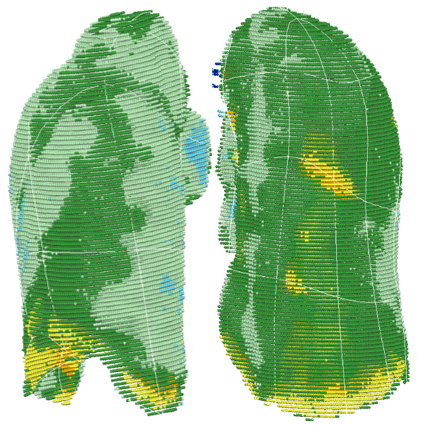
\includegraphics{QuantitativeAnalysis/Image/ClassifiedData_Time1.png}}% get image width, trim={<left> <lower> <right> <upper>}
    \begin{overpic}[height=1.73in,trim={{.0\wd0} {.0\wd0} {.0\wd0} {.0\wd0}},clip]{QuantitativeAnalysis/Image/ClassifiedData_Time1.png}
    \end{overpic}
    \makebox[60pt]{\raisebox{60pt}{\rotatebox[origin=c]{0}{\minibox{Mapped\\ data}}}}% \makebox:change left space, \raisebox: change upper space
    \begin{overpic}[height=1.83in,trim={{.0\wd0} {.0\wd0} {.0\wd0} {.0\wd0}},clip]{QuantitativeAnalysis/Image/MappedData_Time1.png}
    \end{overpic}
    \caption{Time point 1}
		\label{fig:MainMappingResult-a}
\end{subfigure}\hspace{0.3cm}
\begin{subfigure}{4.8cm}
    \sbox0{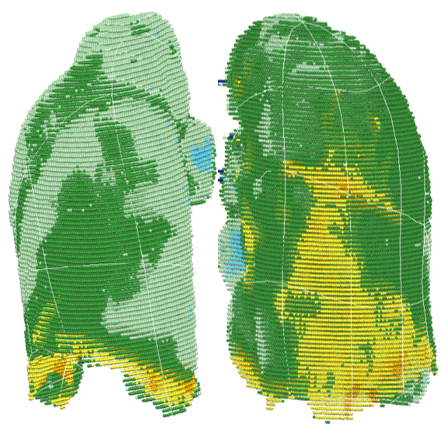
\includegraphics{QuantitativeAnalysis/Image/ClassifiedData_Time2.png}}% get image width, trim={<left> <lower> <right> <upper>}
    \begin{overpic}[height=1.7in,trim={{.0\wd0} {.0\wd0} {.0\wd0} {.0\wd0}},clip]{QuantitativeAnalysis/Image/ClassifiedData_Time2.png}
    \end{overpic}
    \begin{overpic}[height=1.88in,trim={{.0\wd0} {.0\wd0} {.0\wd0} {.0\wd0}},clip]{QuantitativeAnalysis/Image/MappedData_Time2.png}
    \end{overpic}
    \caption{Time point 2}
		\label{fig:MainMappingResult-b}
\end{subfigure}\hspace{0.3cm}
\begin{subfigure}{4.8cm}
    \sbox0{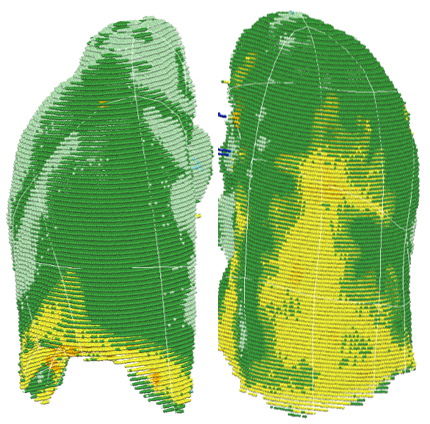
\includegraphics{QuantitativeAnalysis/Image/ClassifiedData_Time3.png}}% get image width, trim={<left> <lower> <right> <upper>}
    \begin{overpic}[height=1.67in,trim={{.0\wd0} {.0\wd0} {.0\wd0} {.0\wd0}},clip]{QuantitativeAnalysis/Image/ClassifiedData_Time3.png}
    \end{overpic}
    \begin{overpic}[height=1.9in,trim={{.0\wd0} {.0\wd0} {.0\wd0} {.0\wd0}},clip]{QuantitativeAnalysis/Image/MappedData_Time3.png}
    \end{overpic}
    \caption{Time point 3}
		\label{fig:MainMappingResult-c}
\end{subfigure}
\begin{subfigure}{2cm}
    \makebox[30pt]{\raisebox{100pt}{\rotatebox[origin=c]{0}{\minibox{\\}}}}
    \sbox0{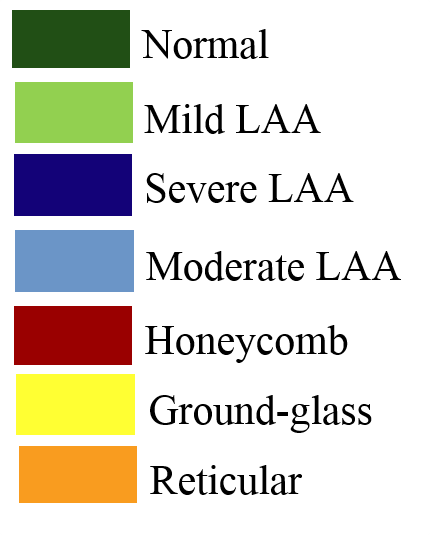
\includegraphics{QuantitativeAnalysis/Image/ClassifiedColor.png}}% get image width, trim={<left> <lower> <right> <upper>}
    \begin{overpic}[height=1.78in,trim={{.0\wd0} {.0\wd0} {.0\wd0} {.0\wd0}},clip]{QuantitativeAnalysis/Image/ClassifiedColor_new.png}
    \end{overpic}
\end{subfigure}
\caption{Classified data (top row) and mapped data (bottom row) for three time points from one subject diagnosed with IPF. (a) The first time point, scan time: 0 months. (b) The second time point, scan time: 15 months. (c) The third time point, scan time: 20 months.}
\label{fig:MainMappingResult}
\end{figure}
\end{landscape}
\restoregeometry

%Figure \ref{fig:NormalizationResult} shows the slices with gaps and the slices after gap filling for three time points at the same position in the lung.
%
%\begin{figure}[htbp]
%\begin{subfigure}{3.7cm}
    %\makebox[4pt]{\raisebox{50pt}{\rotatebox[origin=c]{0}{\minibox{\\}}}}%
    %\sbox0{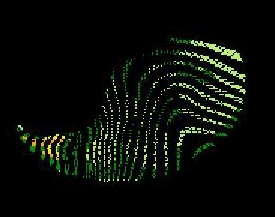
\includegraphics{QuantitativeAnalysis/Image/IPF6_Original_Slice65_1.jpg}}% get image width, trim={<left> <lower> <right> <upper>}
    %\begin{overpic}[height=1.2in,trim={{.0\wd0} {.0\wd0} {.0\wd0} {.0\wd0}},clip]{QuantitativeAnalysis/Image/IPF6_Original_Slice65_1.jpg}
    %\end{overpic}
    %\makebox[4pt]{\raisebox{87pt}{\rotatebox[origin=c]{0}{\minibox{\\}}}}%
    %\begin{overpic}[height=1.2in,trim={{.0\wd0} {.0\wd0} {.0\wd0} {.0\wd0}},clip]{QuantitativeAnalysis/Image/IPF6_Filled_Slice65_1.jpg}
    %\end{overpic}
    %\caption{Time point 1}
		%\label{fig:NormalizationResult-a}
%\end{subfigure}\hspace{.5in}
%\begin{subfigure}{3.7cm}
    %\makebox[4pt]{\raisebox{50pt}{\rotatebox[origin=c]{0}{\minibox{\\}}}}%
    %\sbox0{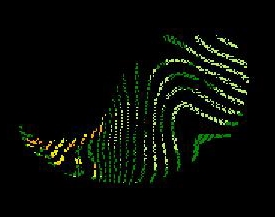
\includegraphics{QuantitativeAnalysis/Image/IPF6_Original_Slice65_2.jpg}}% get image width, trim={<left> <lower> <right> <upper>}
    %\begin{overpic}[height=1.2in,trim={{.0\wd0} {.0\wd0} {.0\wd0} {.0\wd0}},clip]{QuantitativeAnalysis/Image/IPF6_Original_Slice65_2.jpg}
    %\end{overpic}
		%\makebox[4pt]{\raisebox{87pt}{\rotatebox[origin=c]{0}{\minibox{\\}}}}%
    %\begin{overpic}[height=1.2in,trim={{.0\wd0} {.0\wd0} {.0\wd0} {.0\wd0}},clip]{QuantitativeAnalysis/Image/IPF6_Filled_Slice65_2.jpg}
    %\end{overpic}
    %\caption{Time point 2}
		%\label{fig:NormalizationResult-b}
%\end{subfigure}\hspace{.5in}
%\begin{subfigure}{3.7cm}
    %\makebox[4pt]{\raisebox{50pt}{\rotatebox[origin=c]{0}{\minibox{\\}}}}%
    %\sbox0{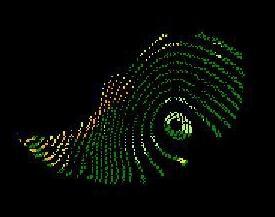
\includegraphics{QuantitativeAnalysis/Image/IPF6_Original_Slice65_3.jpg}}% get image width, trim={<left> <lower> <right> <upper>}
    %\begin{overpic}[height=1.2in,trim={{.0\wd0} {.0\wd0} {.0\wd0} {.0\wd0}},clip]{QuantitativeAnalysis/Image/IPF6_Original_Slice65_3.jpg}
    %\end{overpic}
		%\makebox[4pt]{\raisebox{87pt}{\rotatebox[origin=c]{0}{\minibox{\\}}}}%
    %\begin{overpic}[height=1.2in,trim={{.0\wd0} {.0\wd0} {.0\wd0} {.0\wd0}},clip]{QuantitativeAnalysis/Image/IPF6_Filled_Slice65_3.jpg}
    %\end{overpic}
    %\caption{Time point 3}
		%\label{fig:NormalizationResult-c}
%\end{subfigure}
%\caption{Axial slices with gaps (top row) and axial slices after gap filling (bottom row) of three time points from one subject diagnosed with IPF. (a) The first time point, scan time: 0 month. (b) The second time point, scan time: 5 months. (c) The third time point, scan time: 20 months.}
%\label{fig:NormalizationResult}
%\end{figure}

\subsection{Tissue quantification of IPF lungs}
\subsubsection{Density analysis}
The density analysis result is shown in Figure \ref{fig:LungDensity} and Table \ref{tab:MeanDensity}. It can be seen that the average density of each CT pattern remains consistent and fluctuates only within a specific range over time in both left and right lung. The ground-glass region has the highest average tissue density and emphysema has the lowest average tissue density. This supports that the CALIPER tissue type classification is robust and repeatable.

\begin{table}[htbp]
\centering
\caption{Mean tissue density ($g/c\mathrm{m^3}$) of each CT pattern for left and right lung (mean value $\pm$ standard deviation)}
\label{tab:MeanDensity}
\begin{tabular}{|l | c | c|}
\hline
& \bf{Mean tissue density (left lung)} & \bf{Mean tissue density (right lung)} \\ 
\hline
\bf{Normal} & 0.28$\pm$0.02 & 0.27$\pm$0.01 \\
\hline
\bf{Honeycomb} & 0.15$\pm$0.04 & 0.15$\pm$0.03 \\
\hline
\bf{Reticular} & 0.35$\pm$0.05 & 0.32$\pm$0.04 \\
\hline
\bf{Ground-glass} & 0.42$\pm$0.05 & 0.40$\pm$0.02 \\
\hline
\bf{Emphysema} & 0.08$\pm$0.01 & 0.08$\pm$0.02 \\
\hline
\end{tabular}
\end{table}

\newpage

\begin{figure}[H] 
\centering
\begin{subfigure}{.7\linewidth}% set image scale
  \sbox0{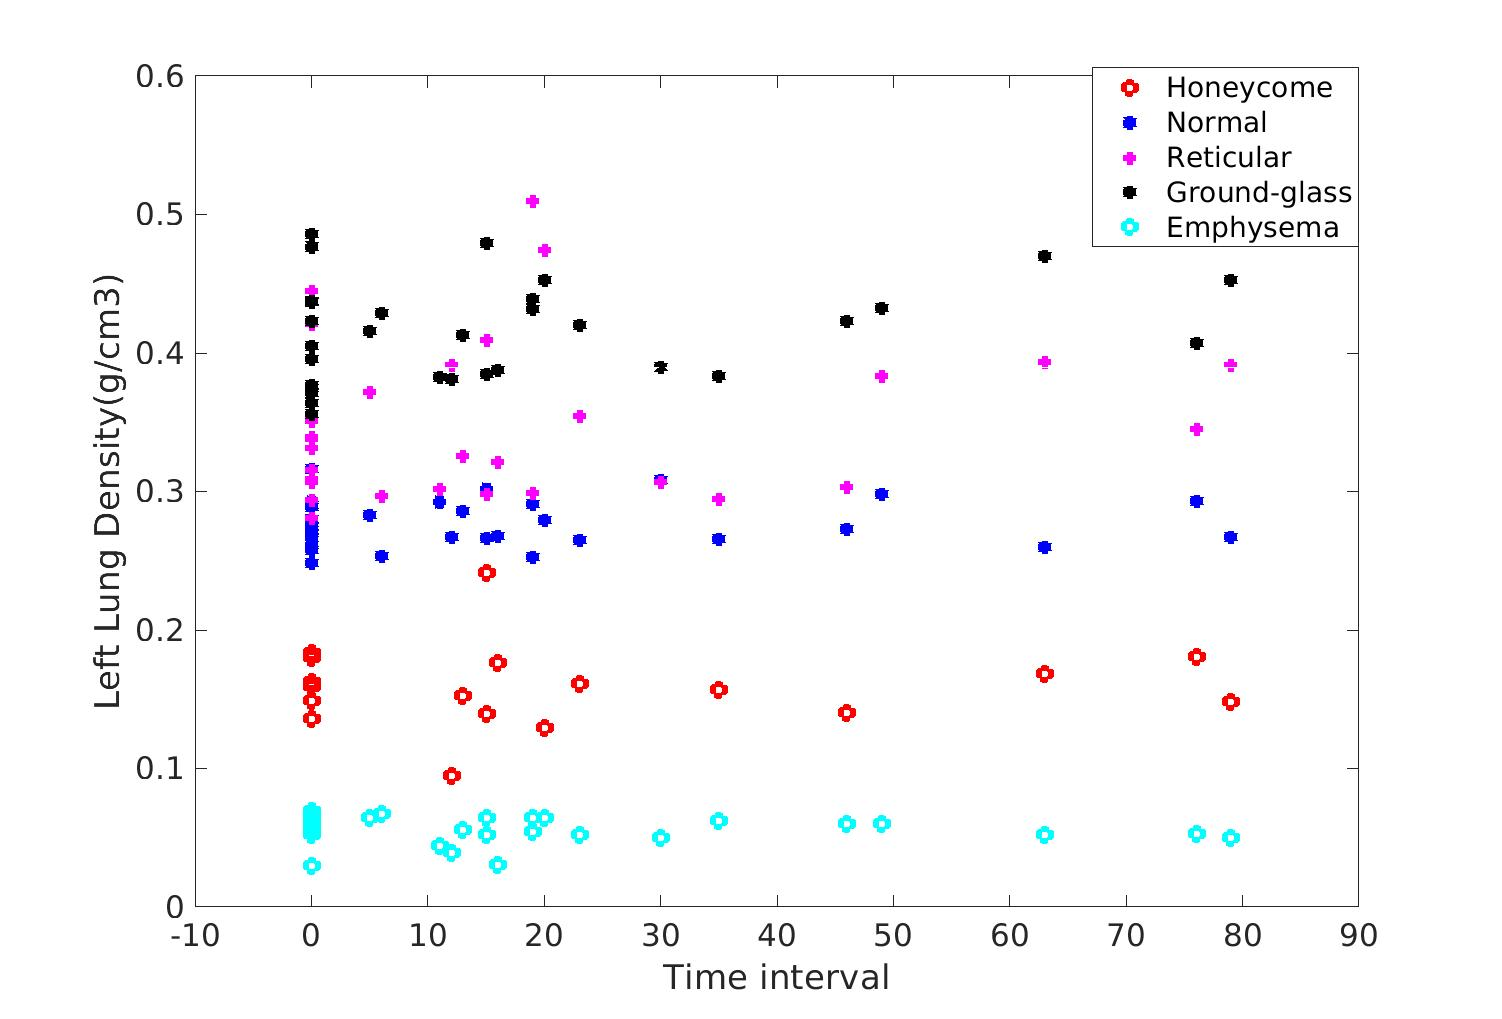
\includegraphics{QuantitativeAnalysis/Image/LeftLungDensity.jpg}} 
  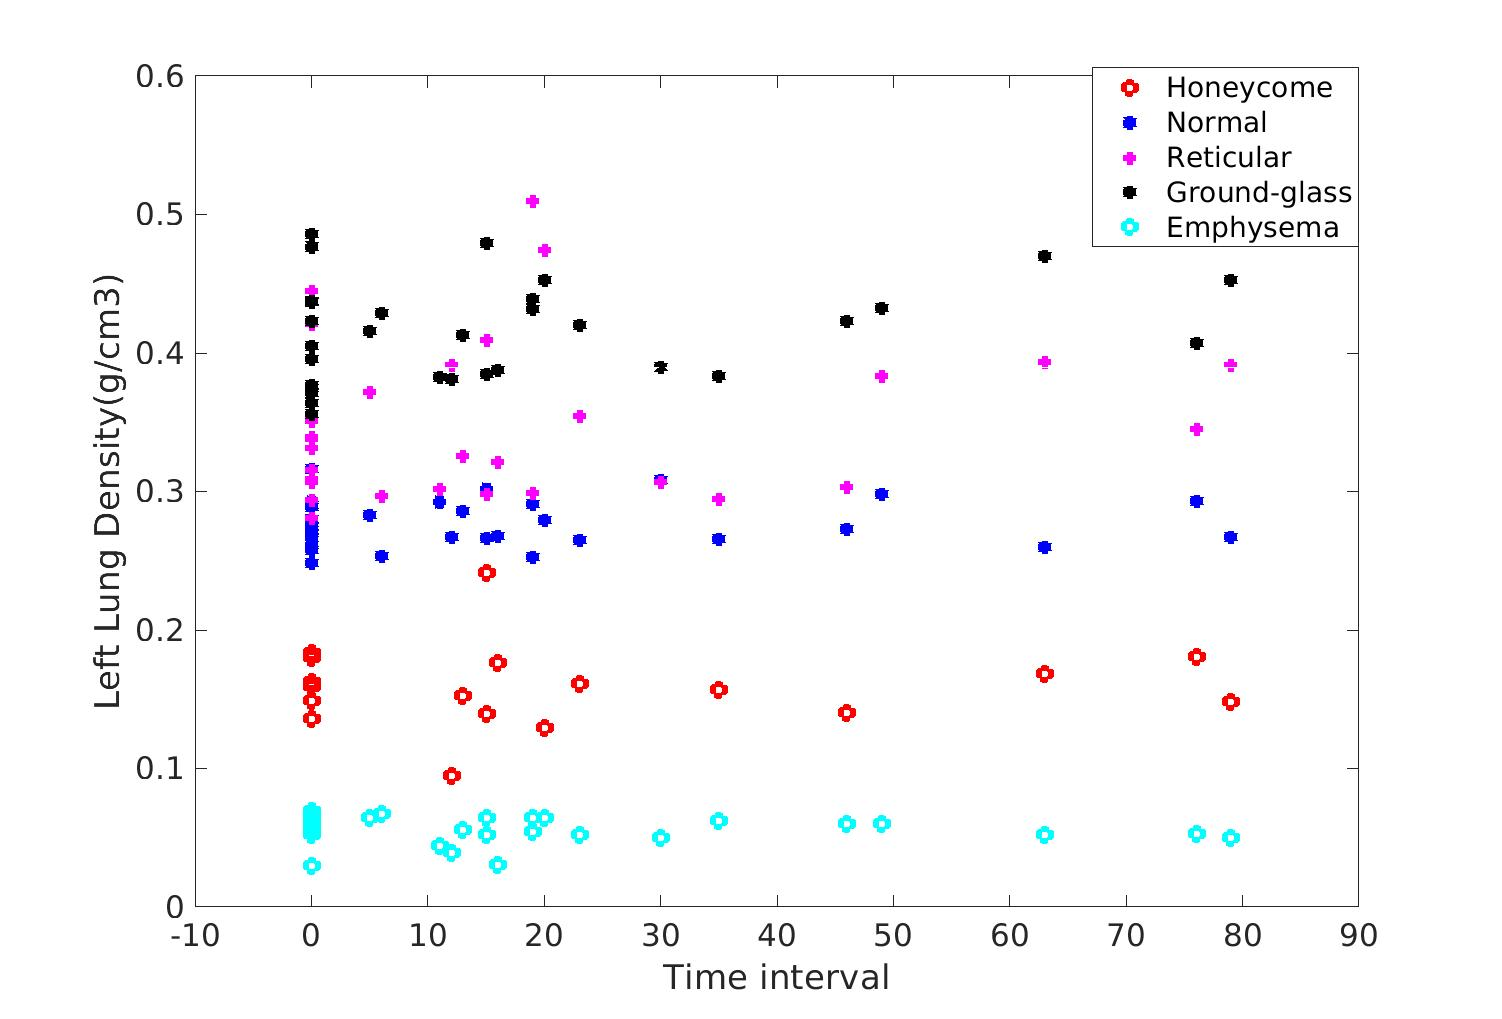
\includegraphics[width=\linewidth,trim={{.0\wd0} {.0\wd0} {.0\wd0} {.0\wd0}},clip]{QuantitativeAnalysis/Image/LeftLungDensity.jpg} %trim={<left> <lower> <right> <upper>}, set the cut scale
  \caption{Left lung tissue density}
  \label{fig:LungDensity-a} 
\end{subfigure} 
\hspace{.3in}
\begin{subfigure}{.7\linewidth}% set image scale
  \sbox0{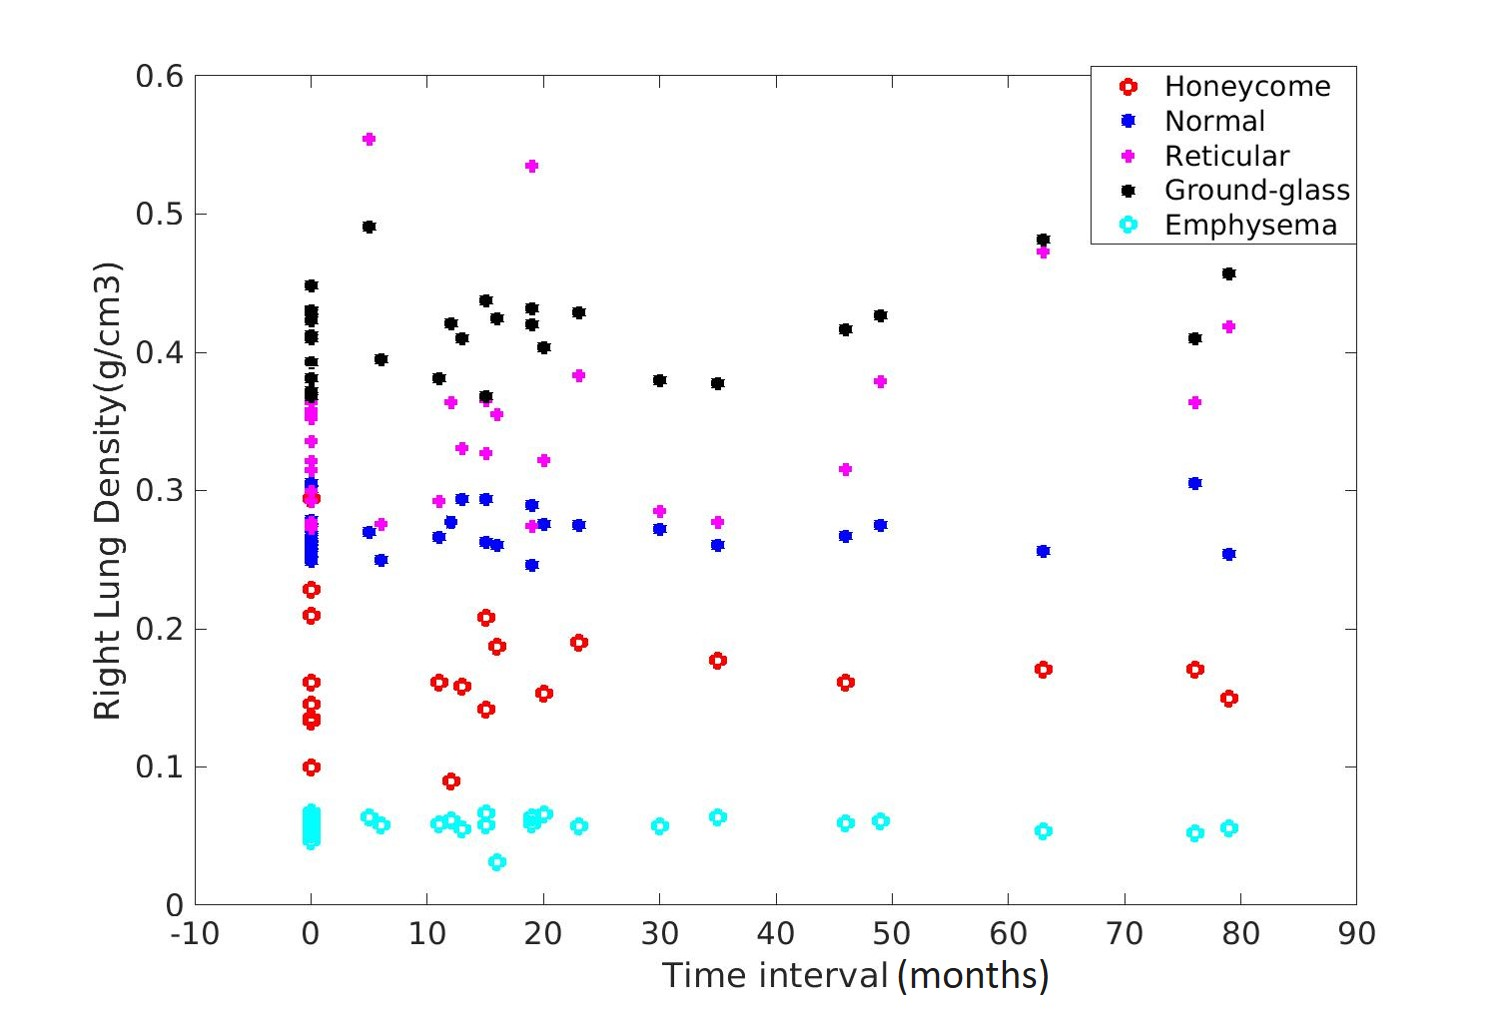
\includegraphics{QuantitativeAnalysis/Image/RightLungDensity.jpg}}
  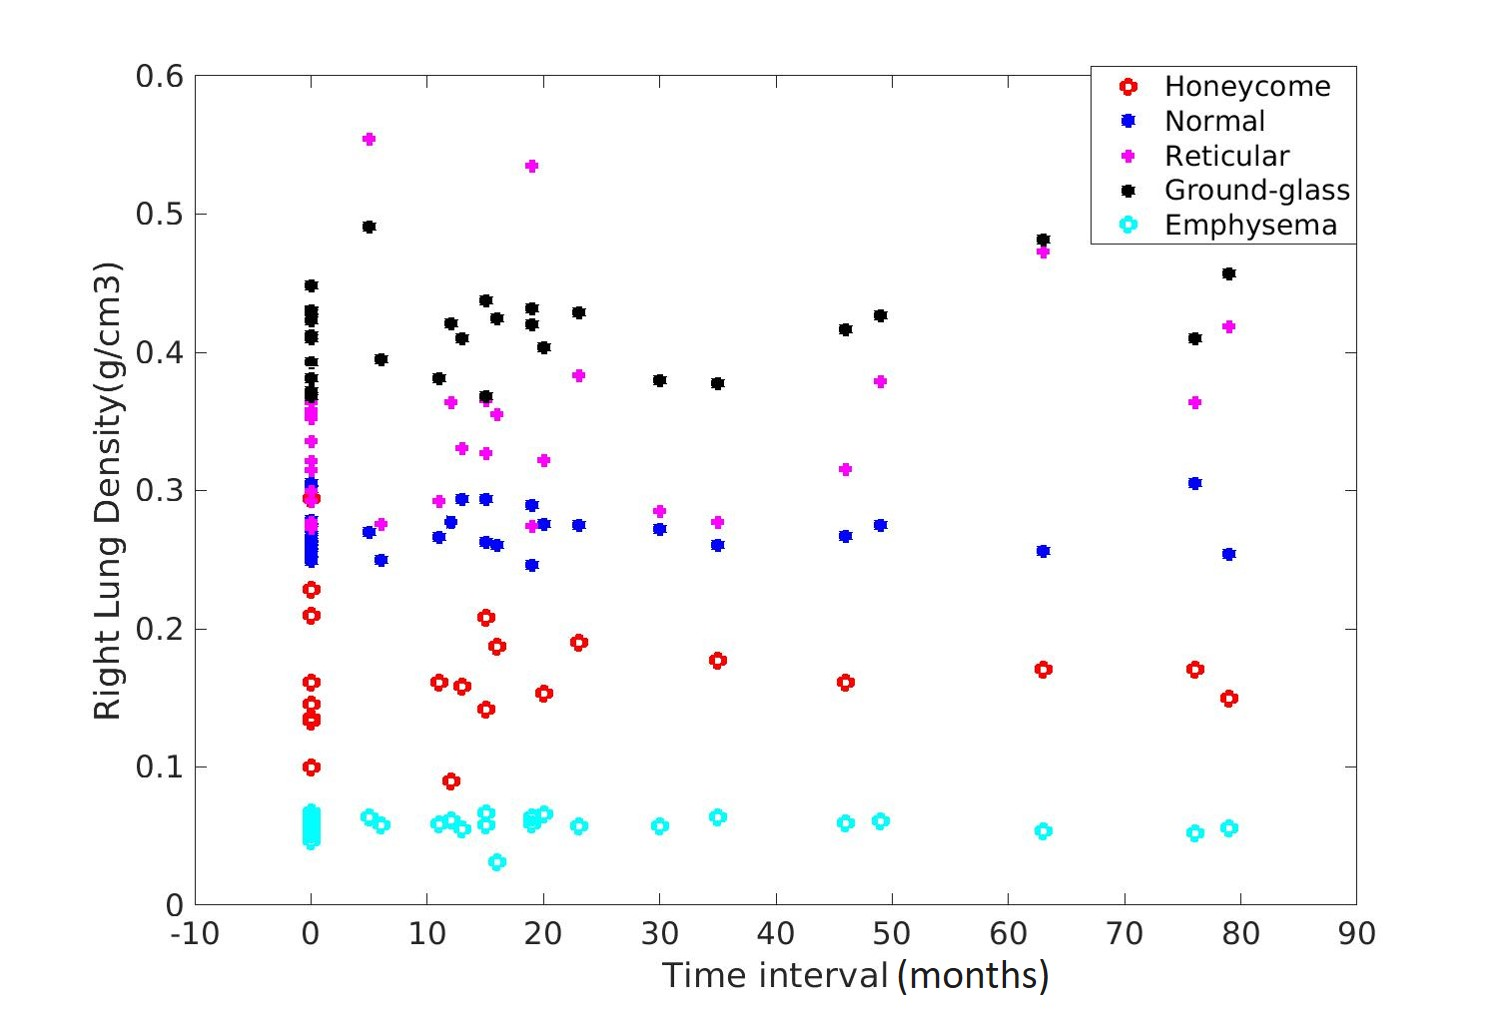
\includegraphics[width=\linewidth,trim={{.0\wd0} {.0\wd0} {.0\wd0} {.0\wd0}},clip]{QuantitativeAnalysis/Image/RightLungDensity.jpg}
  \caption{Right lung tissue density}
  \label{fig:LungDensity-b} 
\end{subfigure}
\caption{Average tissue density (g/c$m^3$) of each CT pattern in IPF lungs. Each data point represents the tissue density of one time point from one patient. X axis represents the month interval of scan time for each patient, and ''0'' represents the first scan for this patient. (a) Tissue density of left lung. (b) Tissue density of right lung.}
\label{fig:LungDensity}
\end{figure}

\subsubsection{Spatial distribution analysis}
\paragraph{Basal-to-apical distribution}
Figure \ref{fig:DiseaseAgainstHeight} shows the percentage distribution (the average volume percentage of all time points from all patients) against lung height (cranio-caudal axis) of four characteristic CT patterns: ground-glass, reticular, honeycomb and emphysema for left and right lung. It can be seen from the result that ground-glass mainly locates in the basal part of the lung. The percentage of ground-glass decreases gradually with increasing lung height, and the distribution of ground-glass is quite similar in left and right lung. In contrast, the percentage of emphysema trends toward increasing from lung base to apex. The reticular tissue is mainly located in the most basal and apical areas: it is much lower in the middle part of the lung. The distribution of honeycomb does not have a relationship with lung height.

Figure \ref{fig:DiseaseAgainstHeightTime1} shows the percentage distribution at month 0 (the average volume percentage of the first time point from all patients) against lung height (cranio-caudal axis) of four characteristic CT patterns (ground-glass, reticular, honeycomb and emphysema) in left and right lung at month 0. From the result, the cranio-caudal distribution of the four CT patterns at month 0 are quite similar to the total average distribution shown in Figure \ref{fig:DiseaseAgainstHeight}, but the absolute percentages of the abnormalities at month 0 are lower than the total average values. That is, as expected, the volume of disease increases over time as a whole in the IPF lung. 
\newpage

\begin{figure}[H] 
\centering
\begin{subfigure}{.42\linewidth}% set image scale
  \sbox0{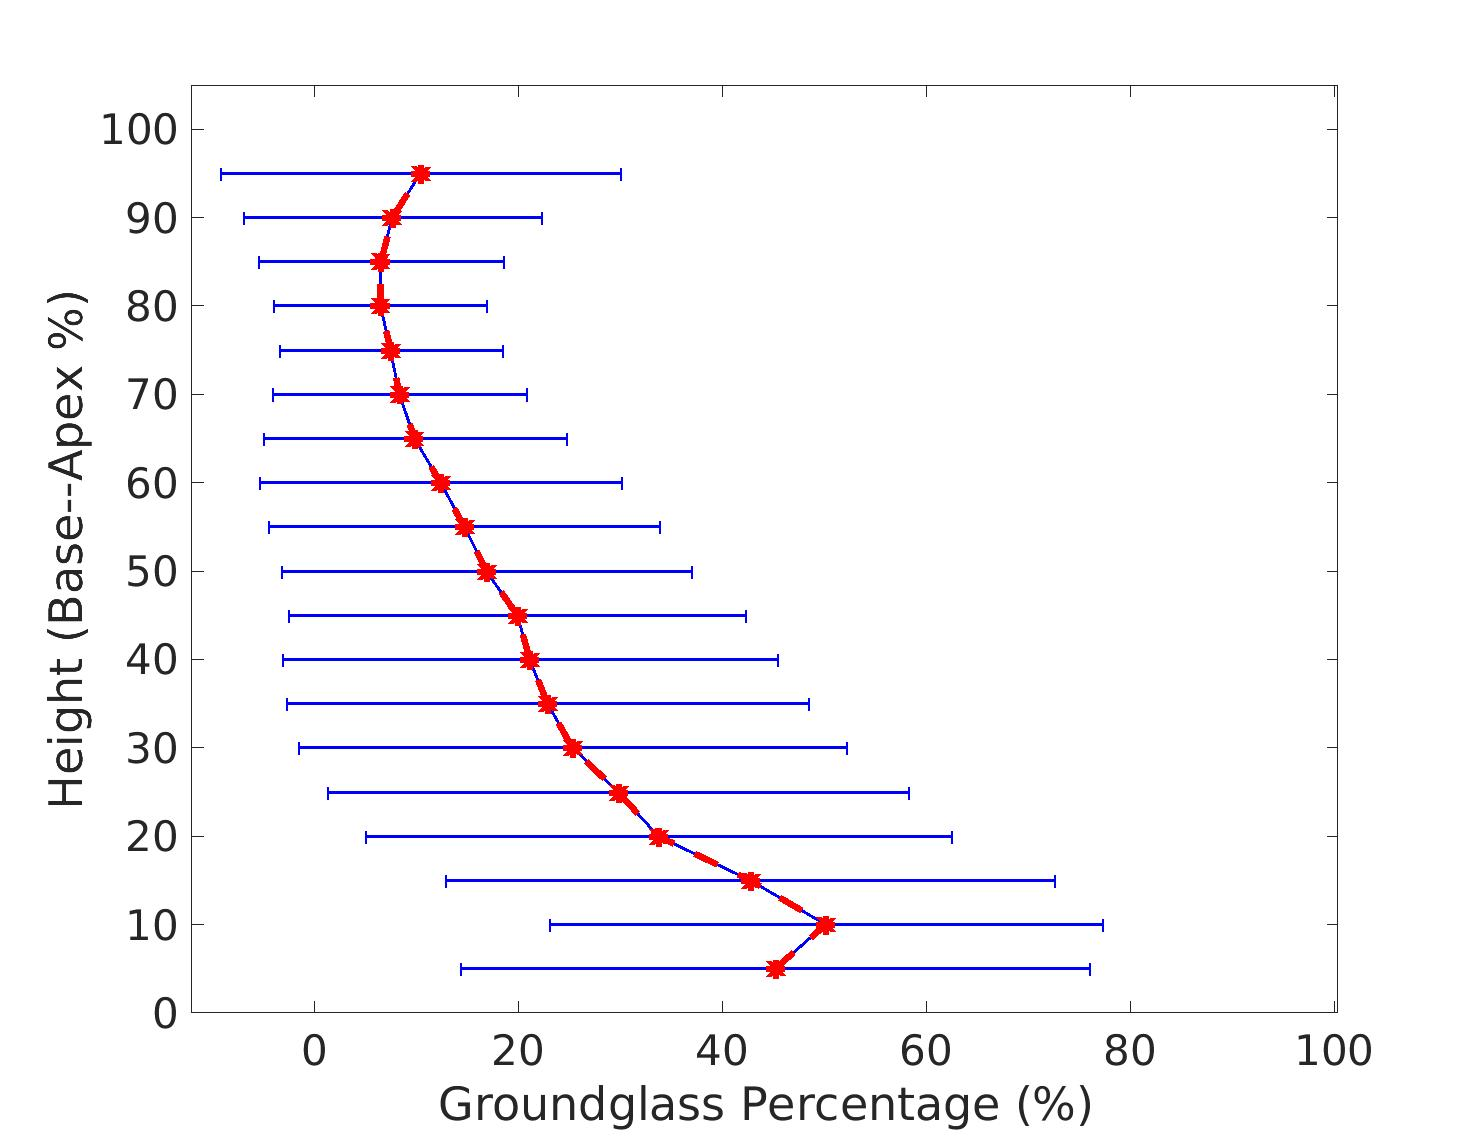
\includegraphics{QuantitativeAnalysis/Image/LeftLungGroundglassDiseaseAgainstHeight.jpg}} 
  %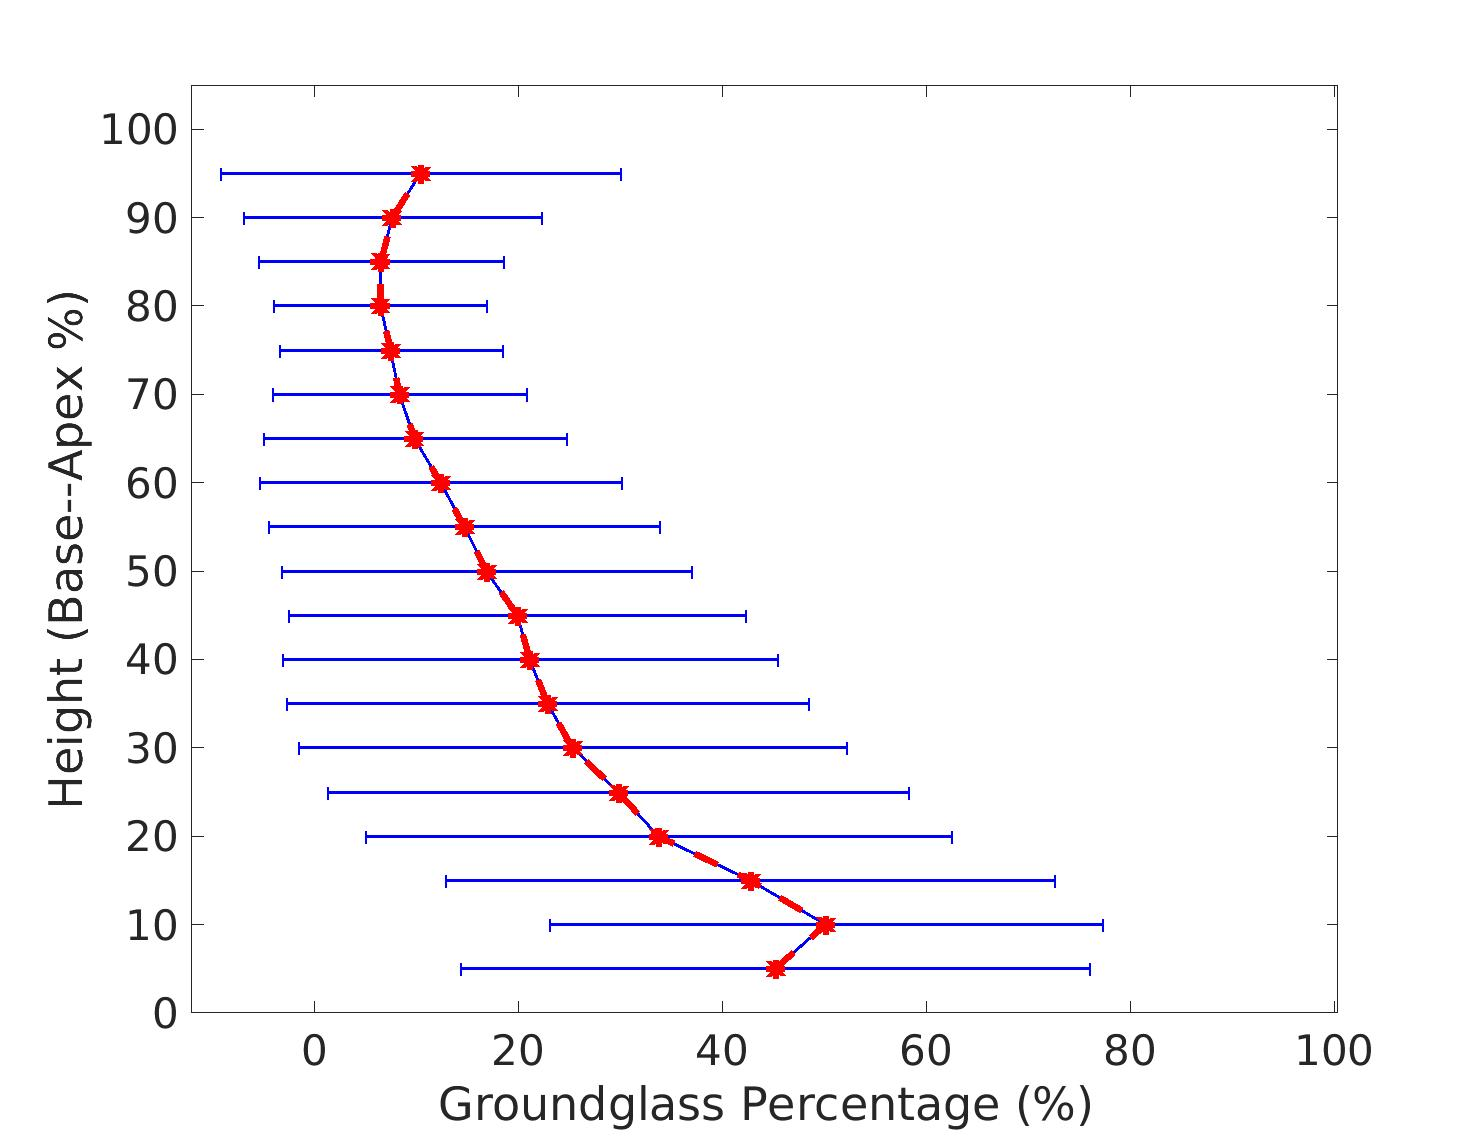
\includegraphics[width=\linewidth,trim={{.0\wd0} {.0\wd0} {.0\wd0} {.0\wd0}},clip]{QuantitativeAnalysis/Image/LeftLungGroundglassDiseaseAgainstHeight.jpg} %trim={<left> <lower> <right> <upper>}, set the cut scale
	\begin{overpic}[width=\linewidth,trim={{.0\wd0} {.0\wd0} {.0\wd0} {.0\wd0}},clip]{QuantitativeAnalysis/Image/LeftLungGroundglassDiseaseAgainstHeight.jpg}
      \put(33,75){\bf{Left lung}}
  \end{overpic}
  \caption{Left ground-glass}
  \label{fig:DiseaseAgainstHeight-a} 
\end{subfigure} 
\begin{subfigure}{.42\linewidth}% set image scale
  \sbox0{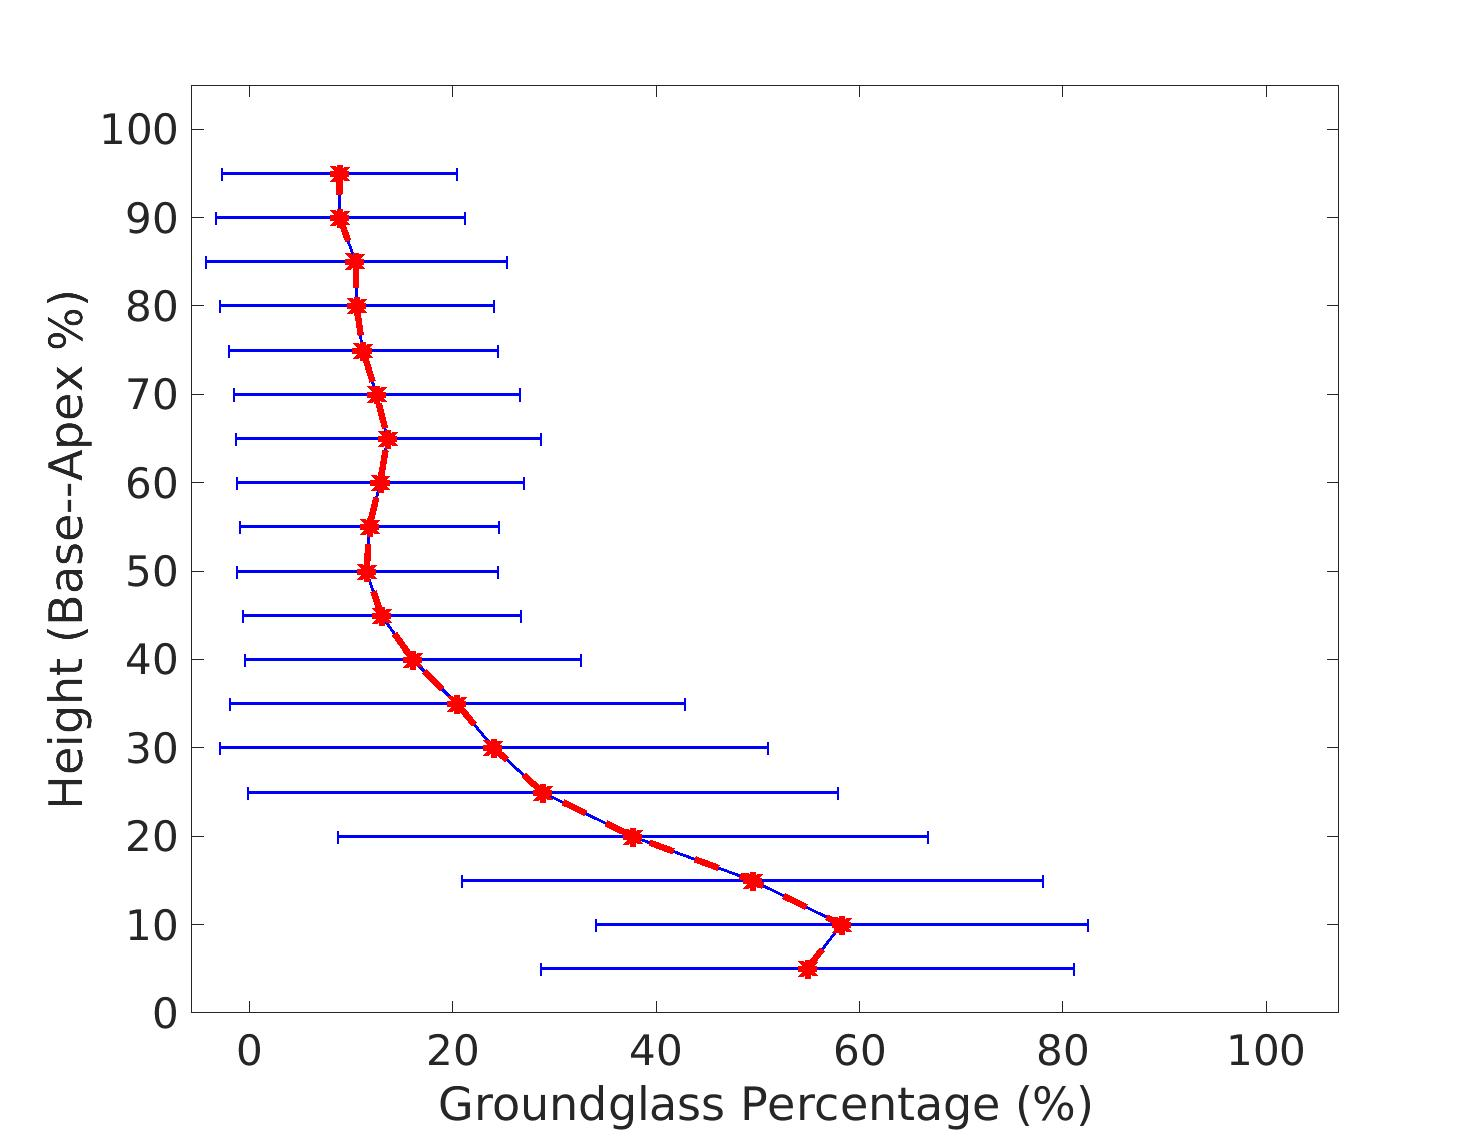
\includegraphics{QuantitativeAnalysis/Image/RightLungGroundglassDiseaseAgainstHeight.jpg}}
  \begin{overpic}[width=\linewidth,trim={{.0\wd0} {.0\wd0} {.0\wd0} {.0\wd0}},clip]{QuantitativeAnalysis/Image/RightLungGroundglassDiseaseAgainstHeight.jpg}
	\put(41,75){\bf{Right lung}}
  \end{overpic}
  \caption{Right ground-glass}
  \label{fig:DiseaseAgainstHeight-b}
\end{subfigure}
\begin{subfigure}{.42\linewidth}% set image scale
  \sbox0{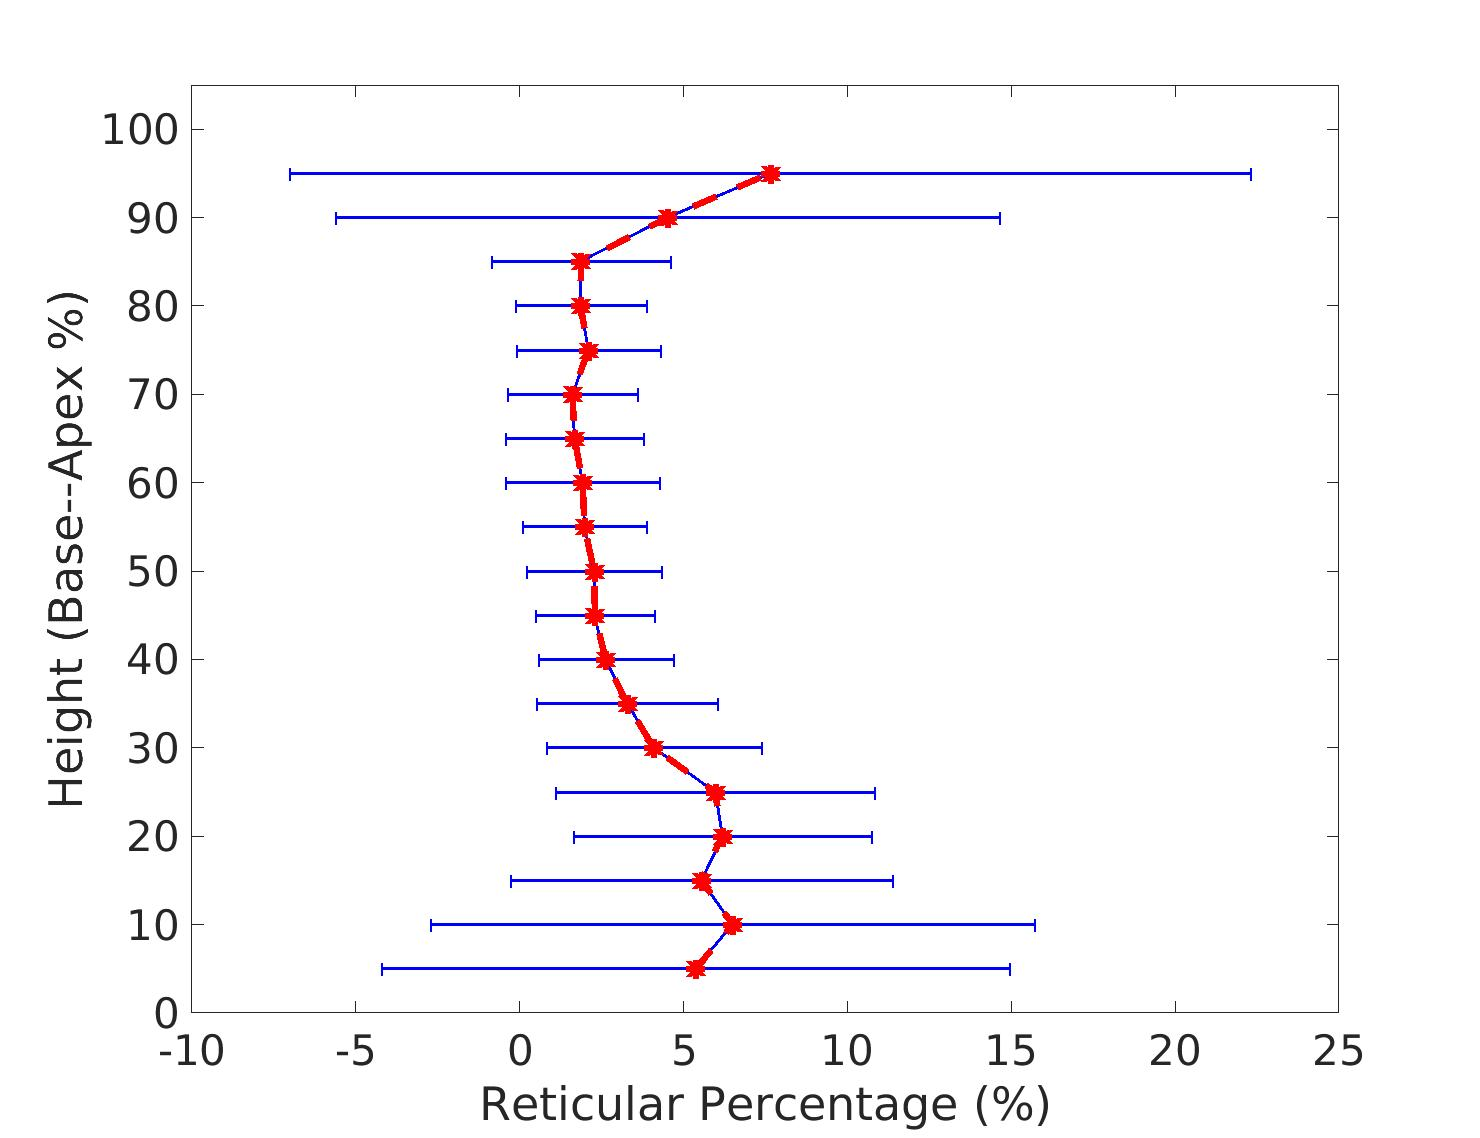
\includegraphics{QuantitativeAnalysis/Image/LeftLungReticularDiseaseAgainstHeight.jpg}} 
  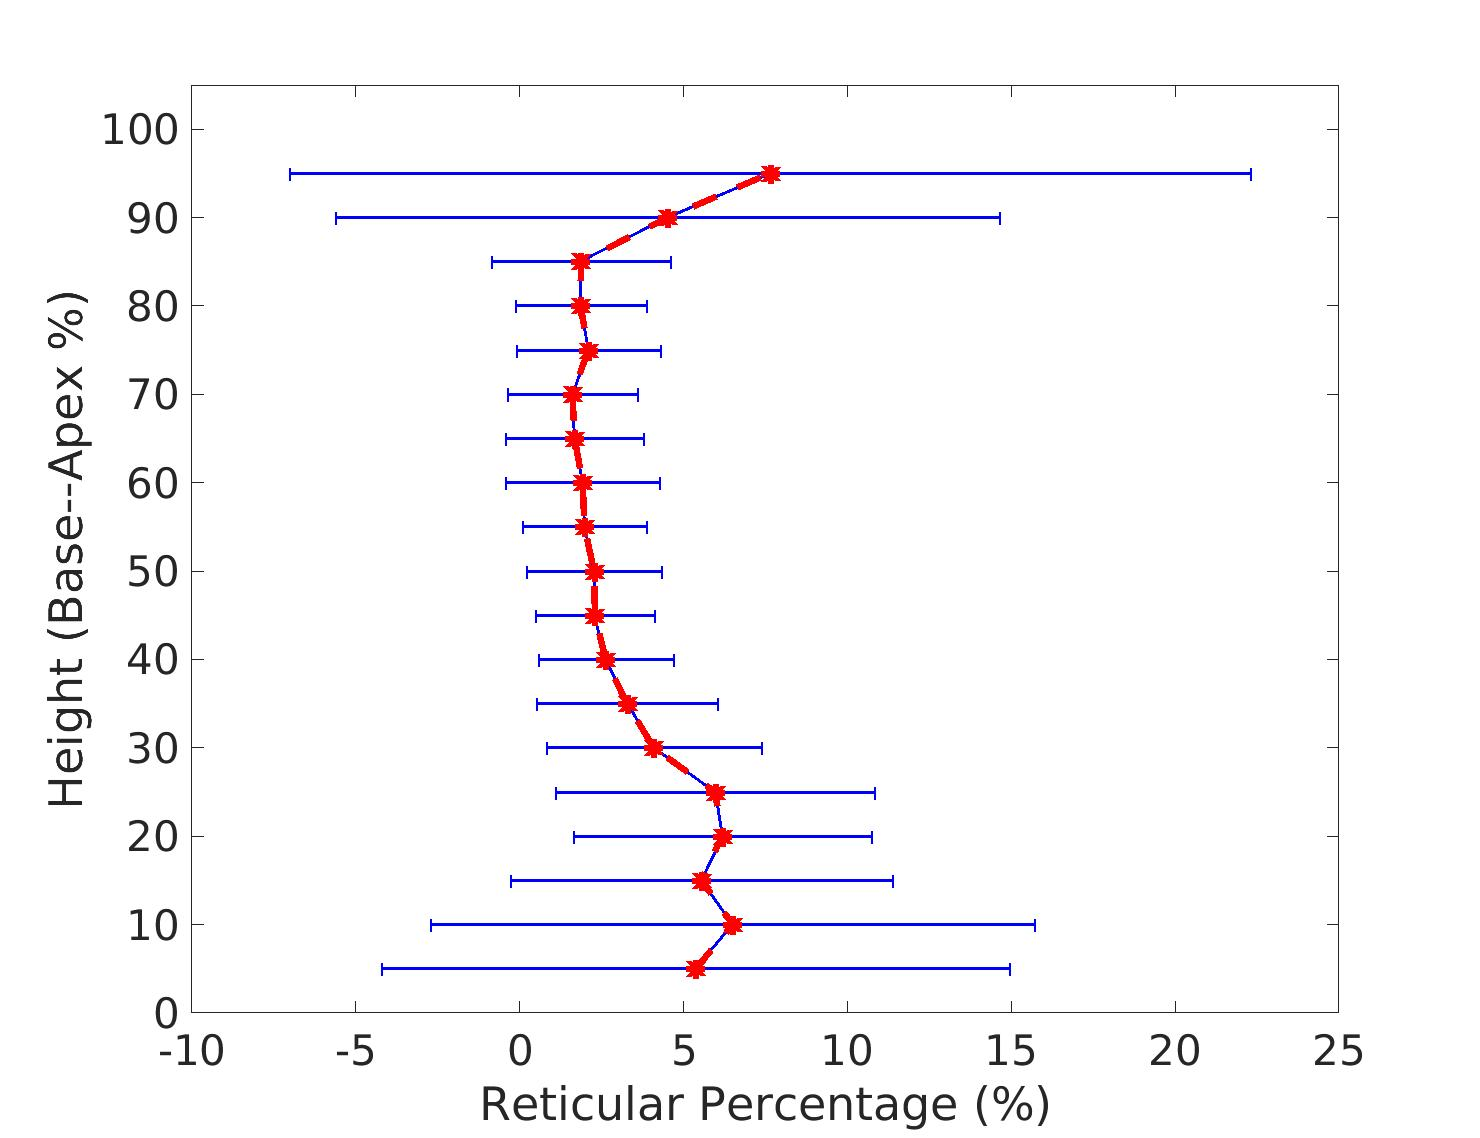
\includegraphics[width=\linewidth,trim={{.0\wd0} {.0\wd0} {.0\wd0} {.0\wd0}},clip]{QuantitativeAnalysis/Image/LeftLungReticularDiseaseAgainstHeight.jpg} %trim={<left> <lower> <right> <upper>}, set the cut scale
  \caption{Left reticular}
  \label{fig:DiseaseAgainstHeight-c} 
\end{subfigure} 
\begin{subfigure}{.42\linewidth}% set image scale
  \sbox0{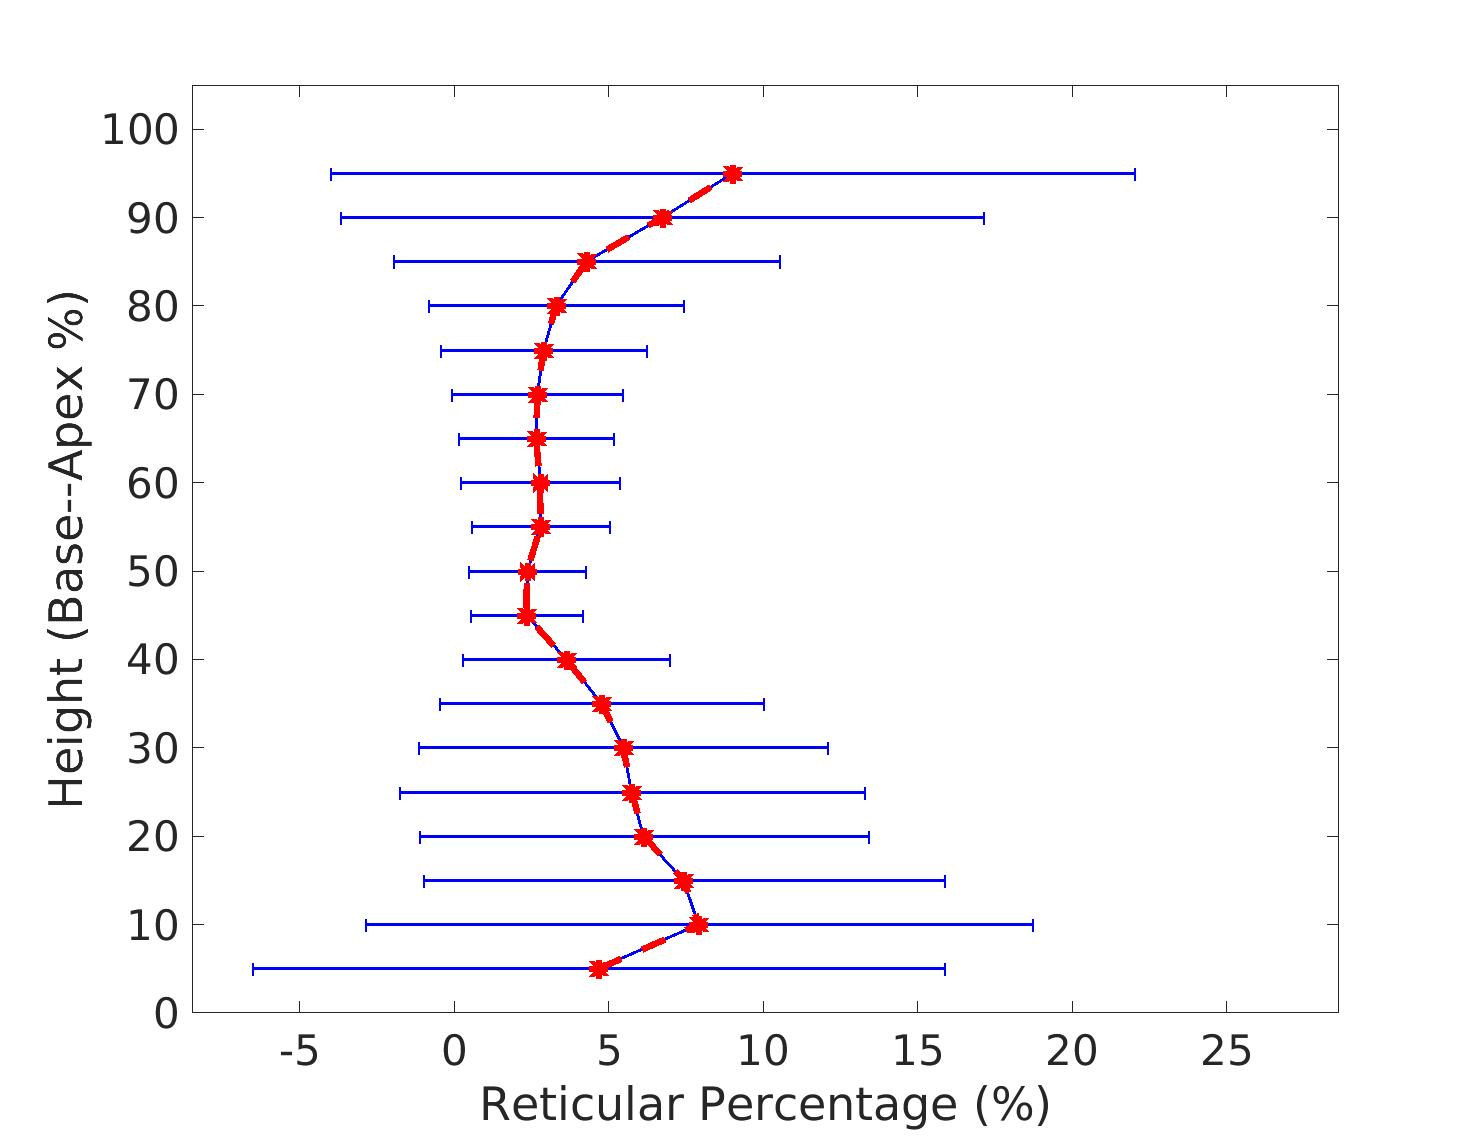
\includegraphics{QuantitativeAnalysis/Image/RightLungReticularDiseaseAgainstHeight.jpg}}
  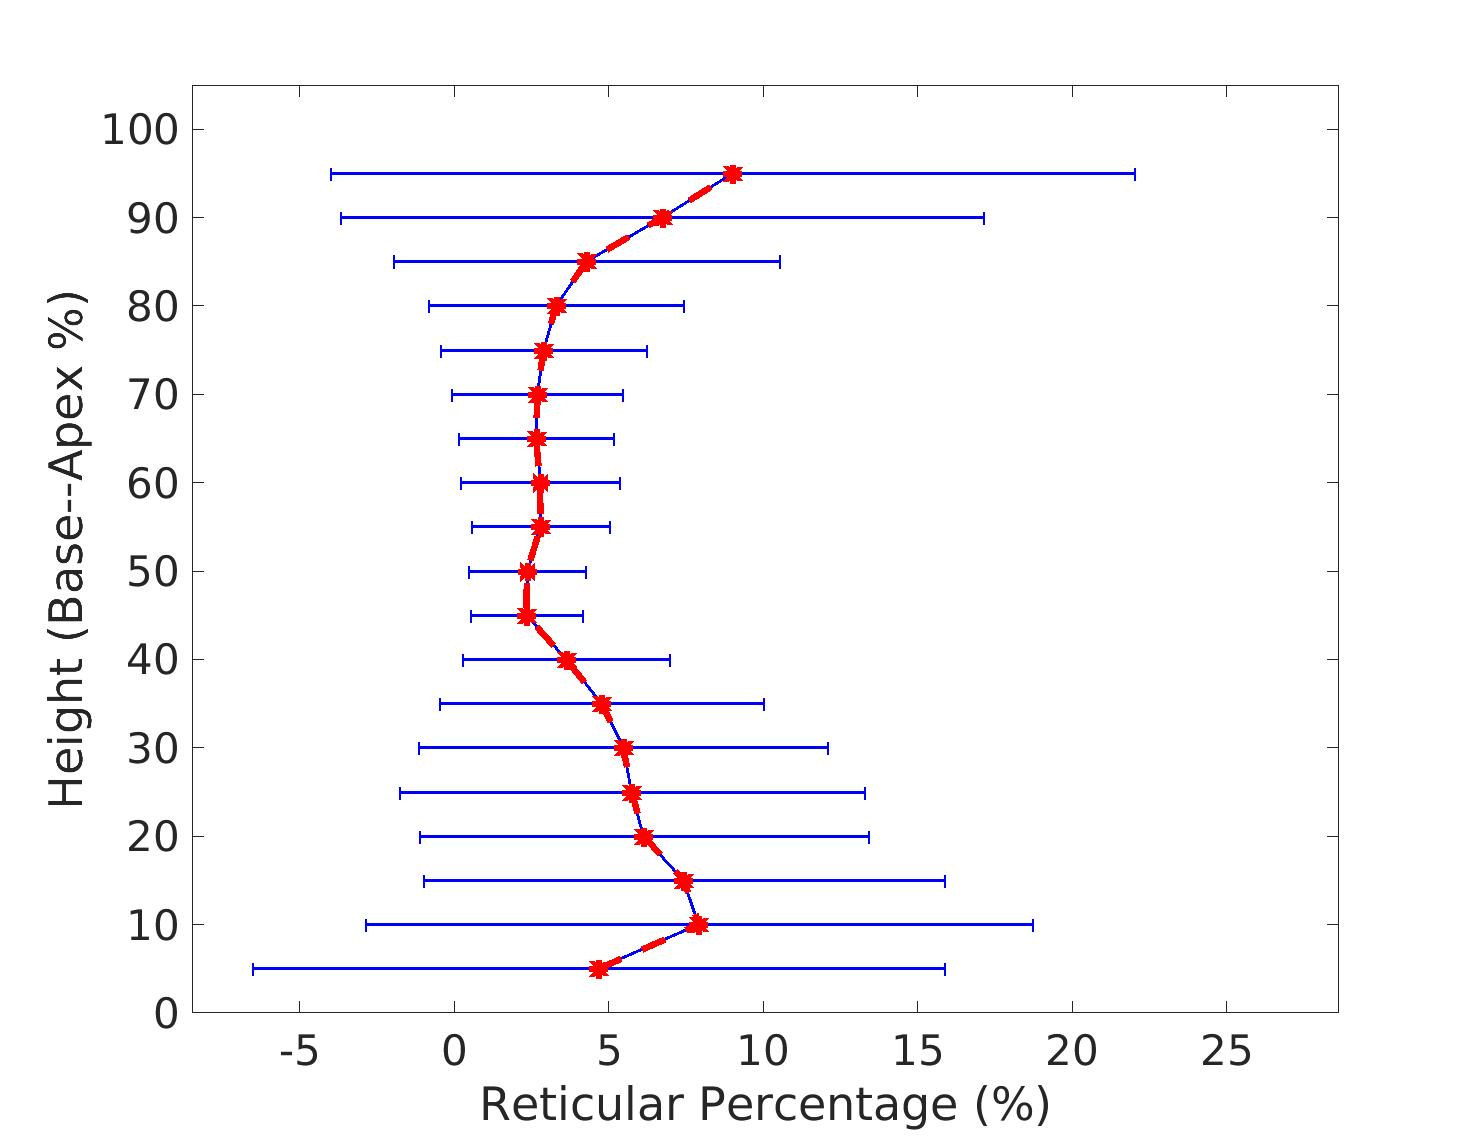
\includegraphics[width=\linewidth,trim={{.0\wd0} {.0\wd0} {.0\wd0} {.0\wd0}},clip]{QuantitativeAnalysis/Image/RightLungReticularDiseaseAgainstHeight.jpg}
  \caption{Right reticular}
  \label{fig:DiseaseAgainstHeight-d}
\end{subfigure}
\begin{subfigure}{.42\linewidth}% set image scale
  \sbox0{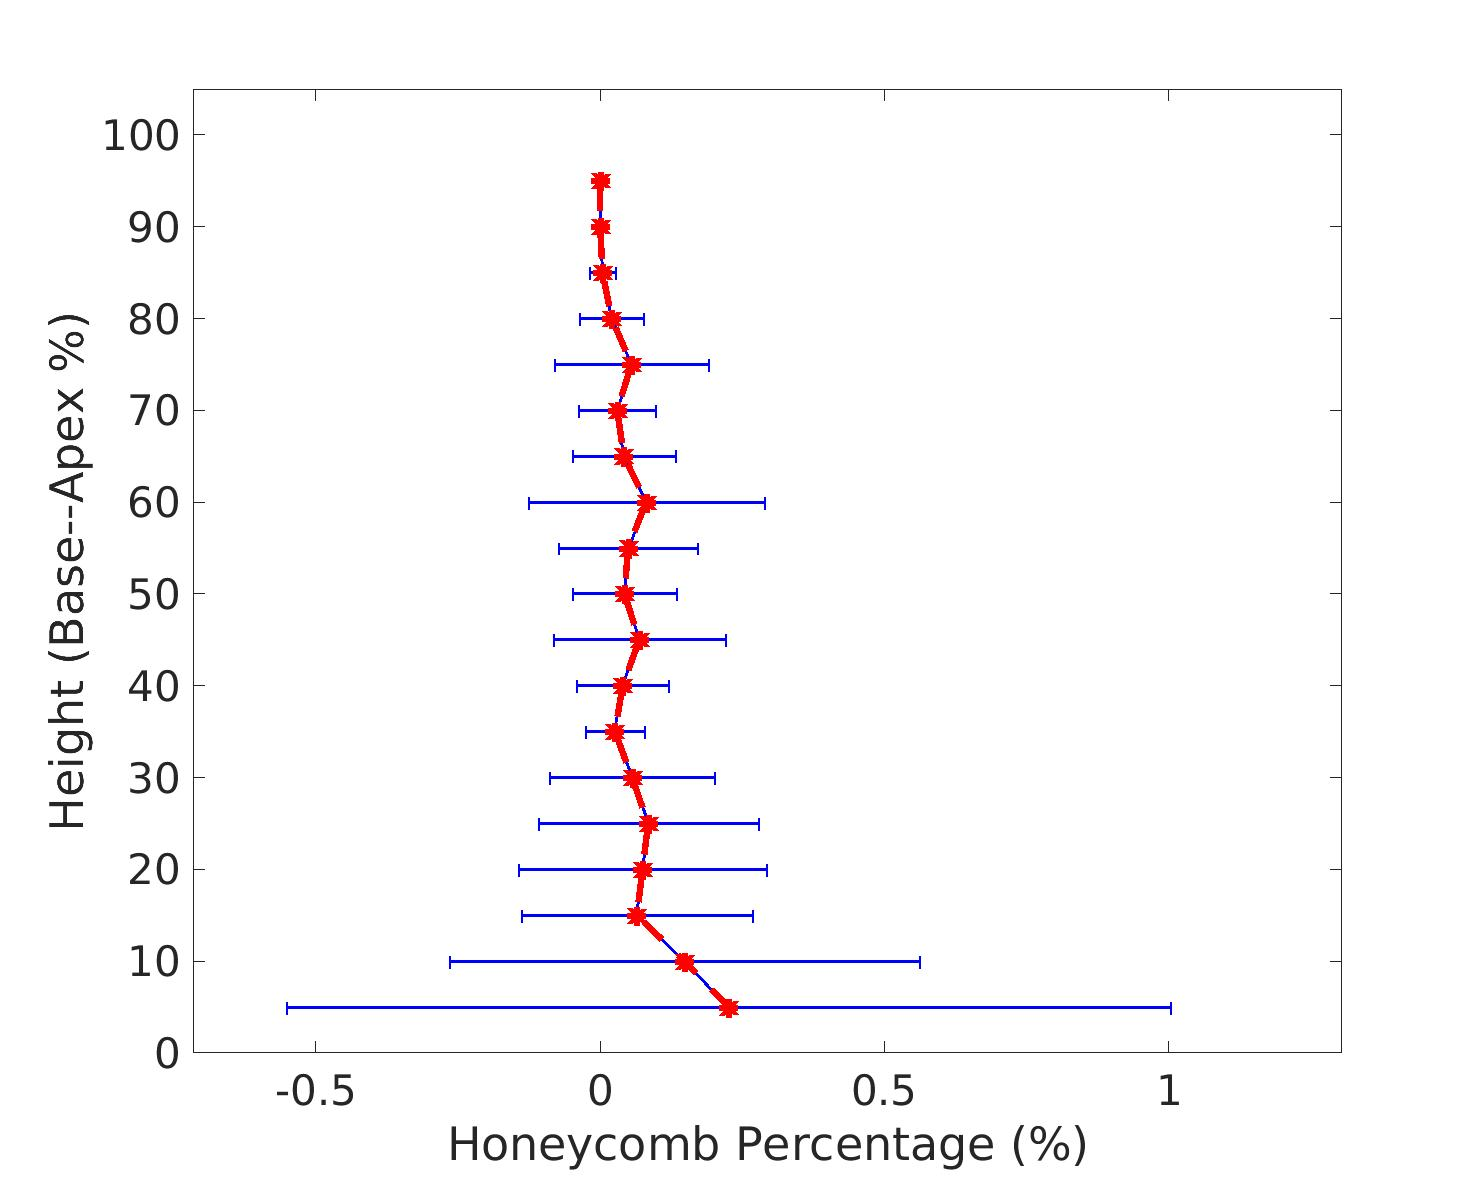
\includegraphics{QuantitativeAnalysis/Image/LeftLungHoneycombDiseaseAgainstHeight.jpg}} 
  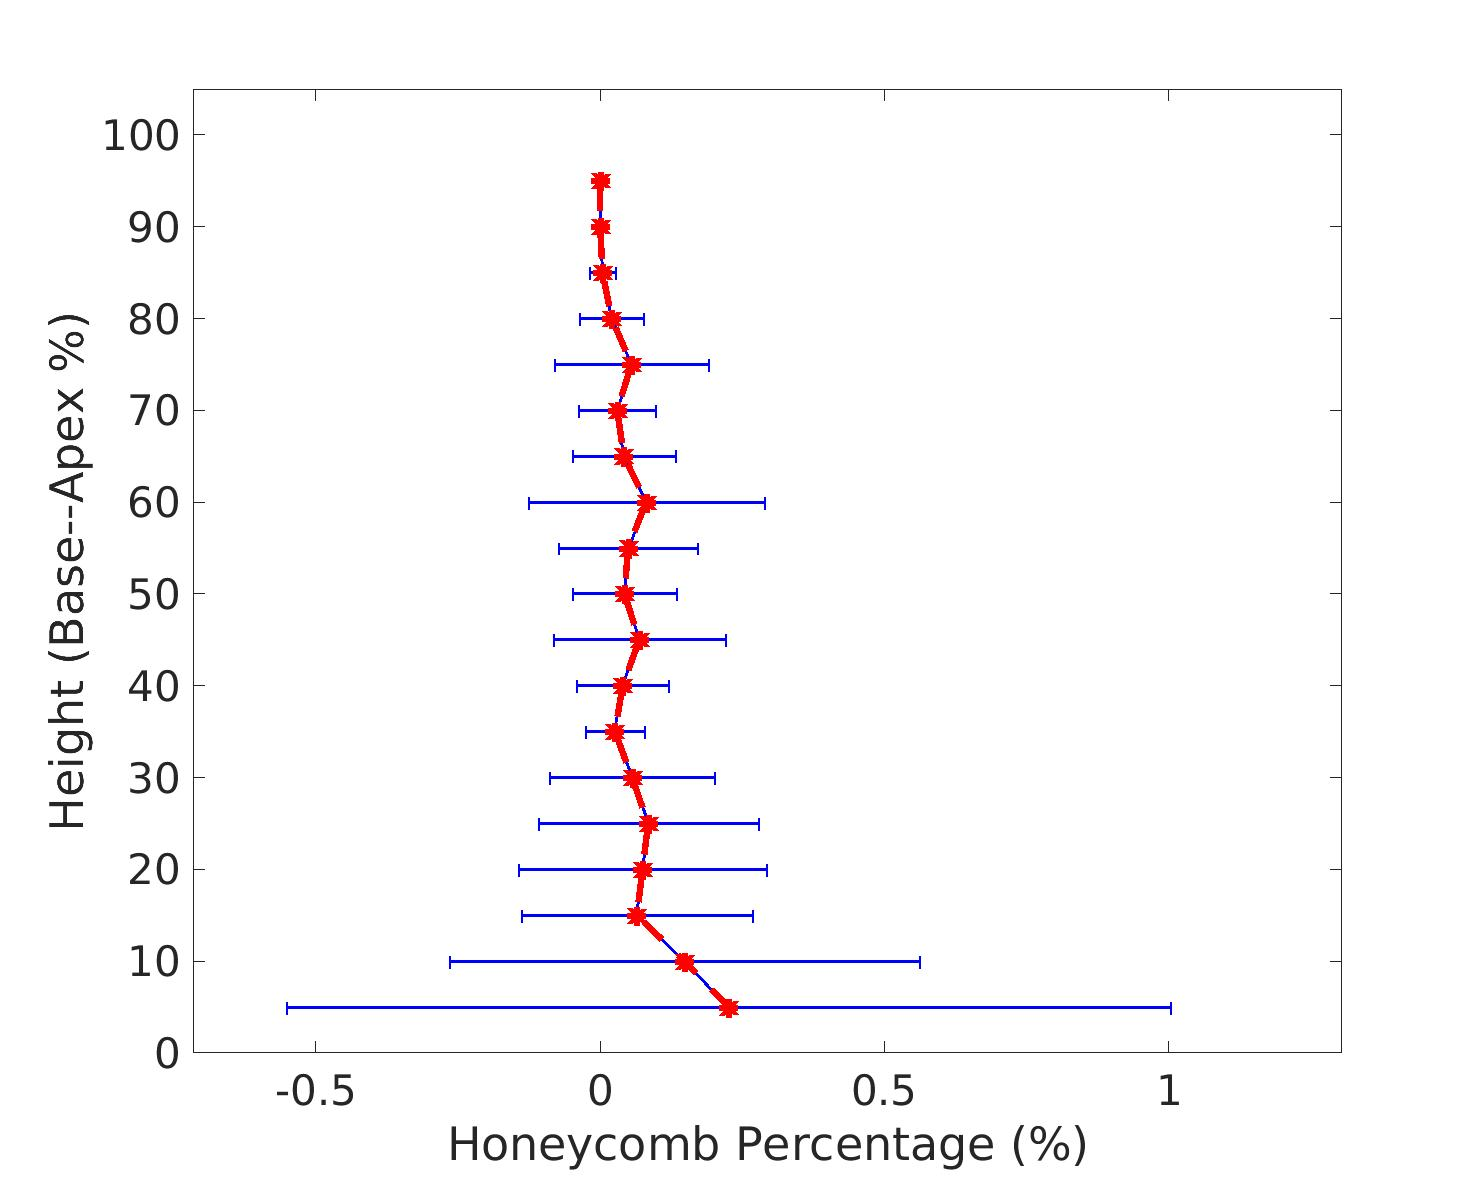
\includegraphics[width=\linewidth,trim={{.0\wd0} {.0\wd0} {.0\wd0} {.0\wd0}},clip]{QuantitativeAnalysis/Image/LeftLungHoneycombDiseaseAgainstHeight.jpg} %trim={<left> <lower> <right> <upper>}, set the cut scale
  \caption{Left honeycomb}
  \label{fig:DiseaseAgainstHeight-e} 
\end{subfigure} 
\begin{subfigure}{.42\linewidth}% set image scale
  \sbox0{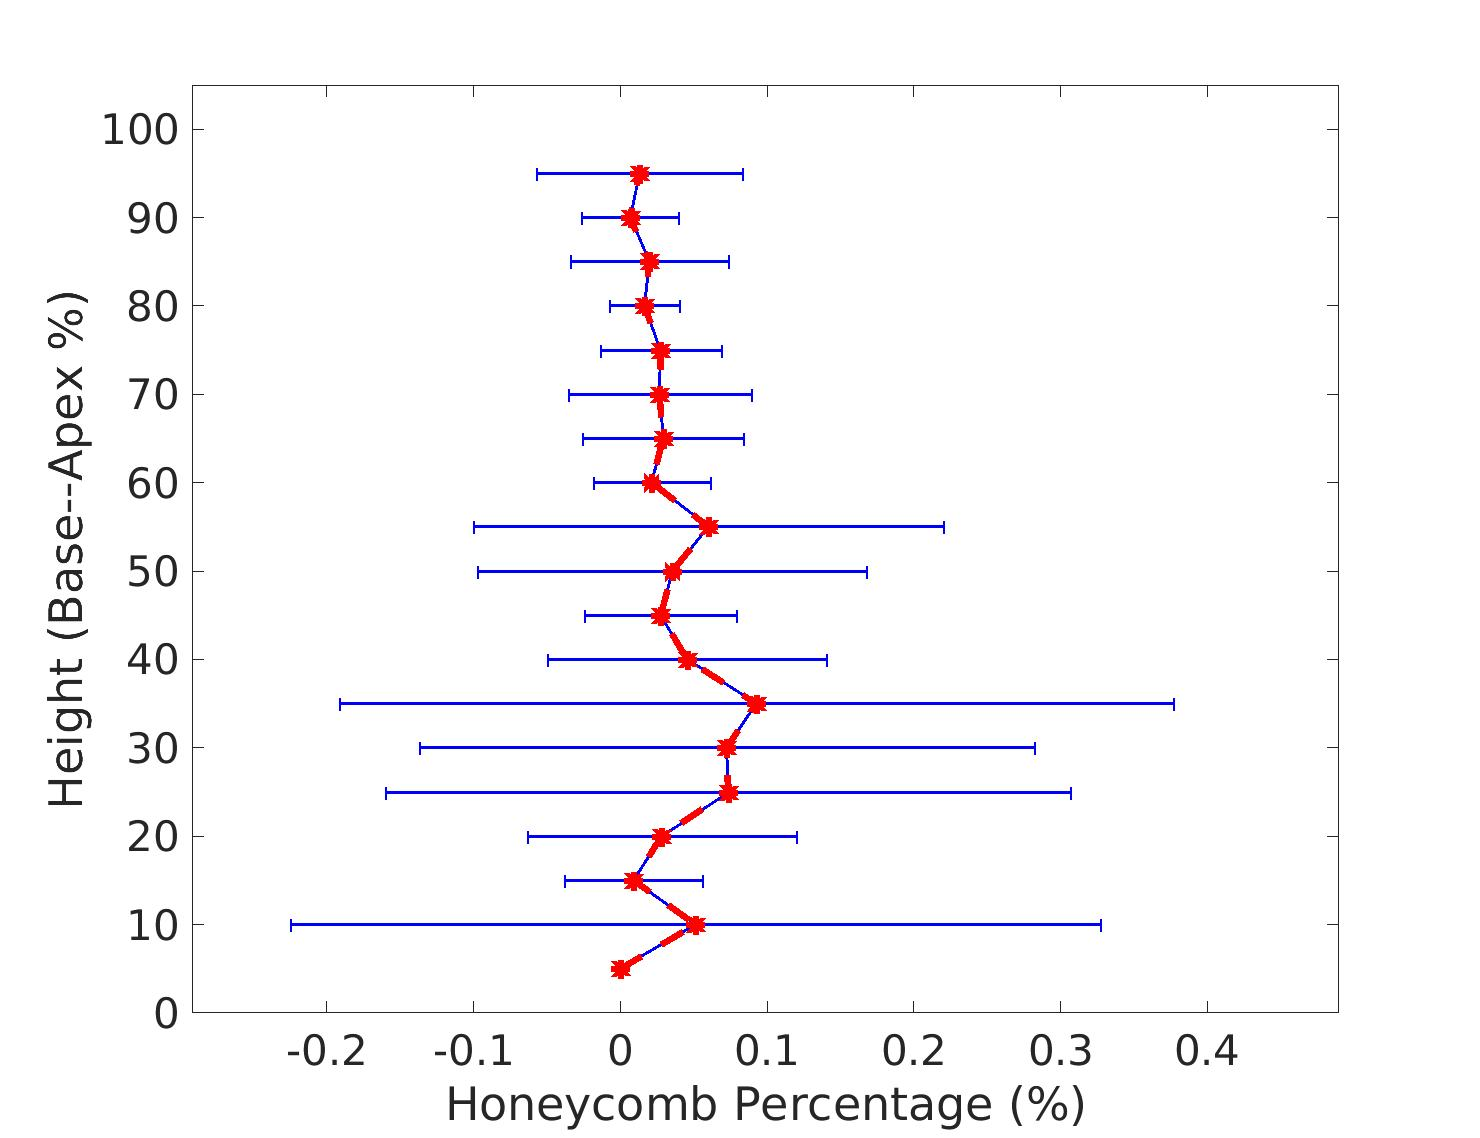
\includegraphics{QuantitativeAnalysis/Image/RightLungHoneycombDiseaseAgainstHeight.jpg}}
  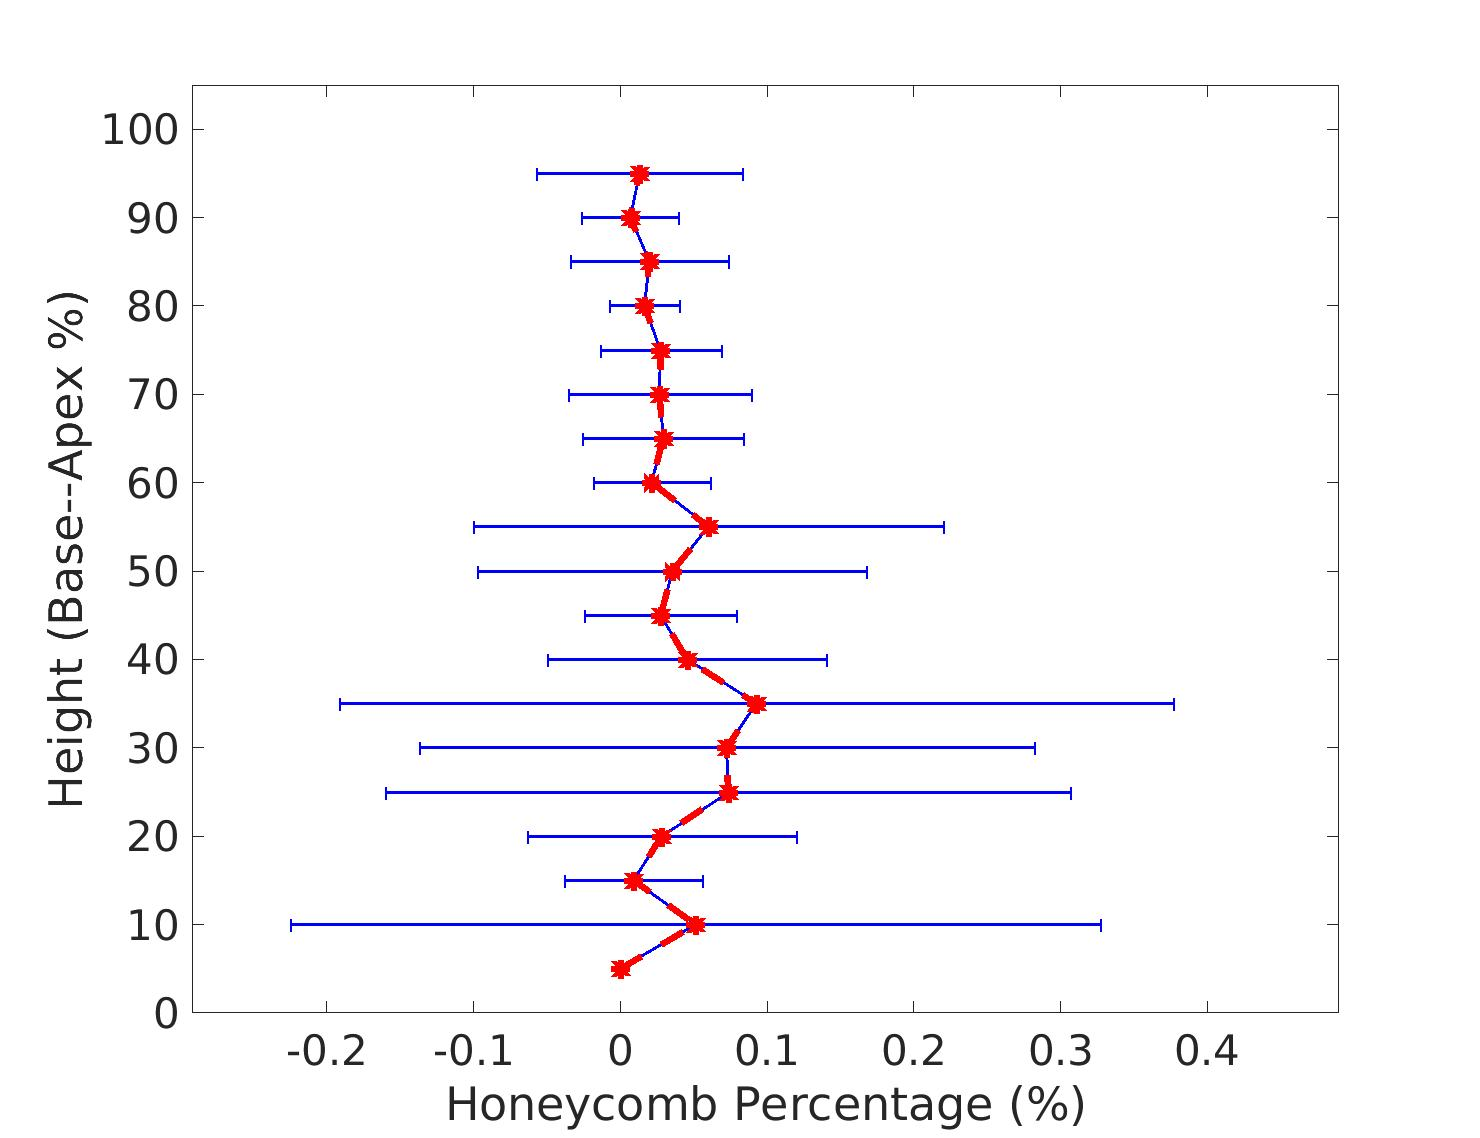
\includegraphics[width=\linewidth,trim={{.0\wd0} {.0\wd0} {.0\wd0} {.0\wd0}},clip]{QuantitativeAnalysis/Image/RightLungHoneycombDiseaseAgainstHeight.jpg}
  \caption{Right honeycomb}
  \label{fig:DiseaseAgainstHeight-f}
\end{subfigure}
\begin{subfigure}{.42\linewidth}% set image scale
  \sbox0{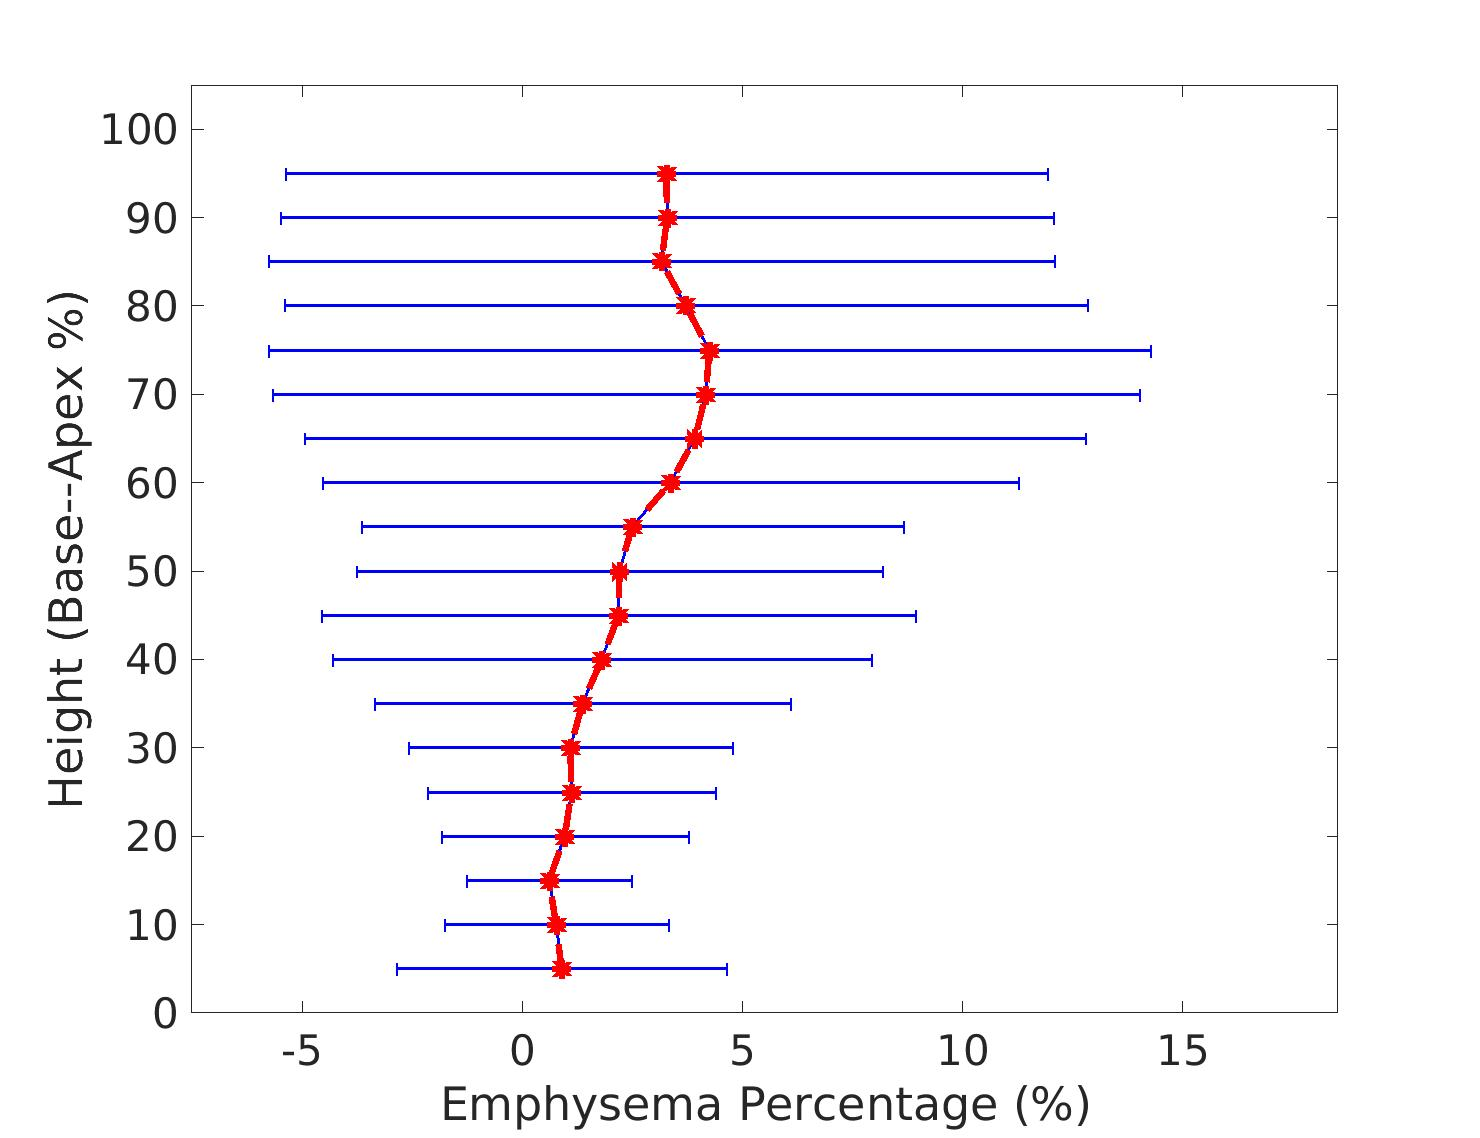
\includegraphics{QuantitativeAnalysis/Image/LeftLungEmphysemaDiseaseAgainstHeight.jpg}} 
  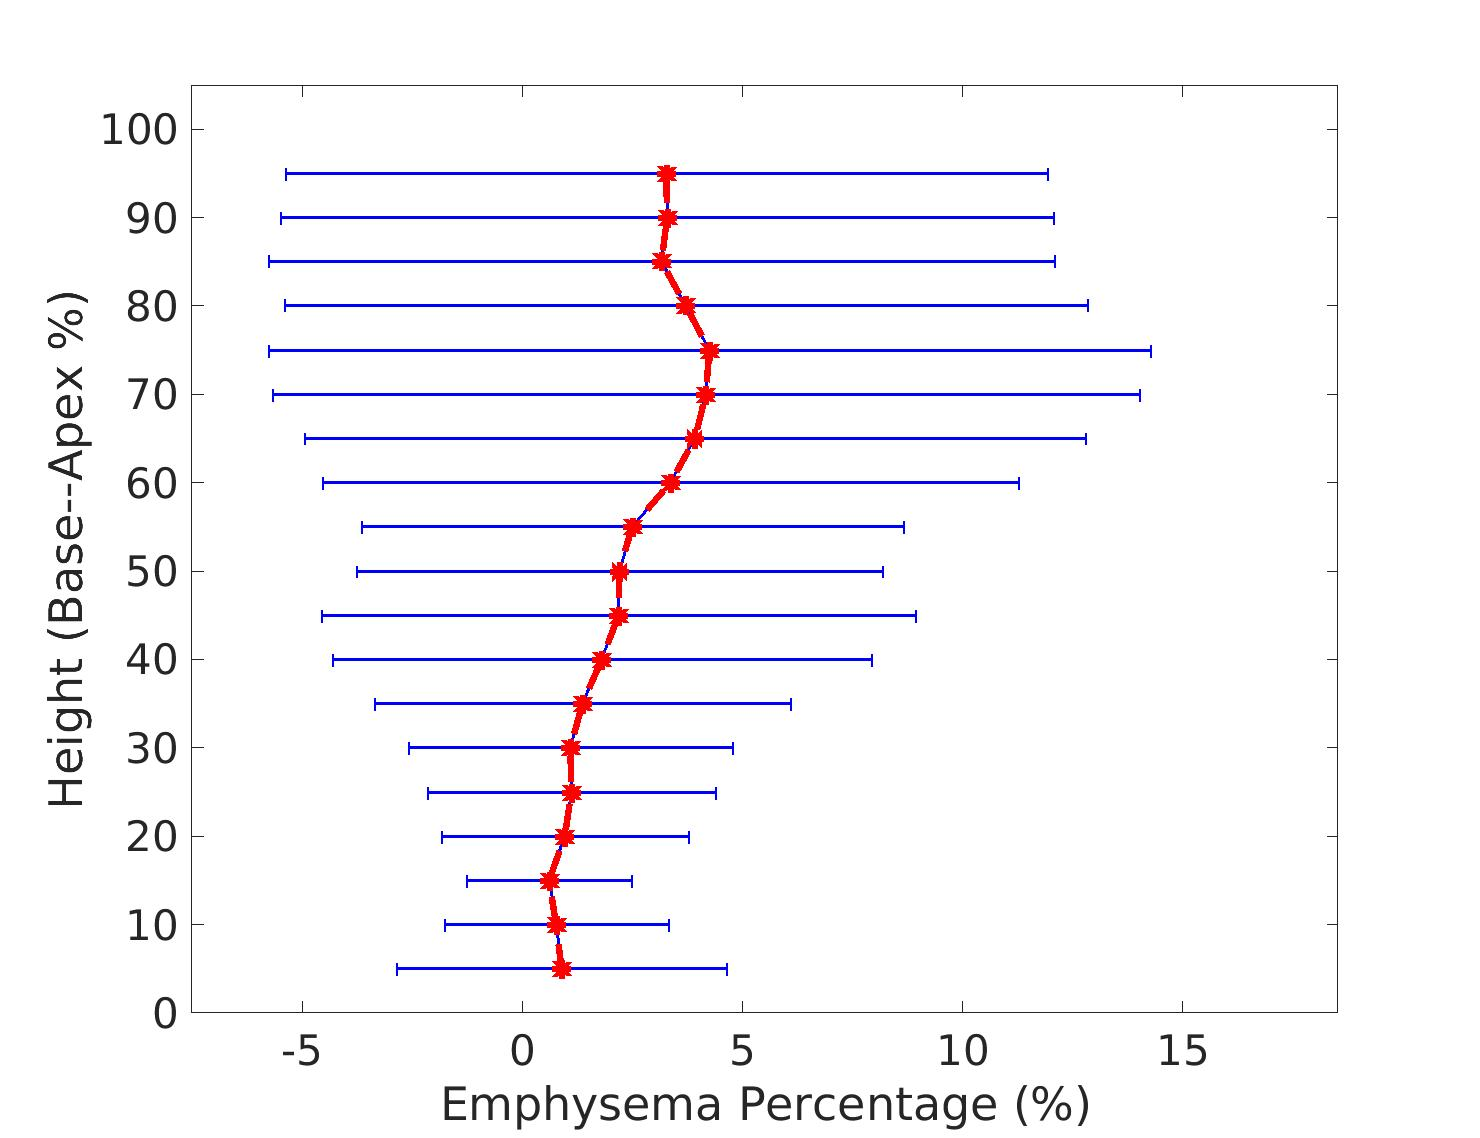
\includegraphics[width=\linewidth,trim={{.0\wd0} {.0\wd0} {.0\wd0} {.0\wd0}},clip]{QuantitativeAnalysis/Image/LeftLungEmphysemaDiseaseAgainstHeight.jpg} %trim={<left> <lower> <right> <upper>}, set the cut scale
  \caption{Left Emphysema}
  \label{fig:DiseaseAgainstHeight-g} 
\end{subfigure} 
\begin{subfigure}{.42\linewidth}% set image scale
  \sbox0{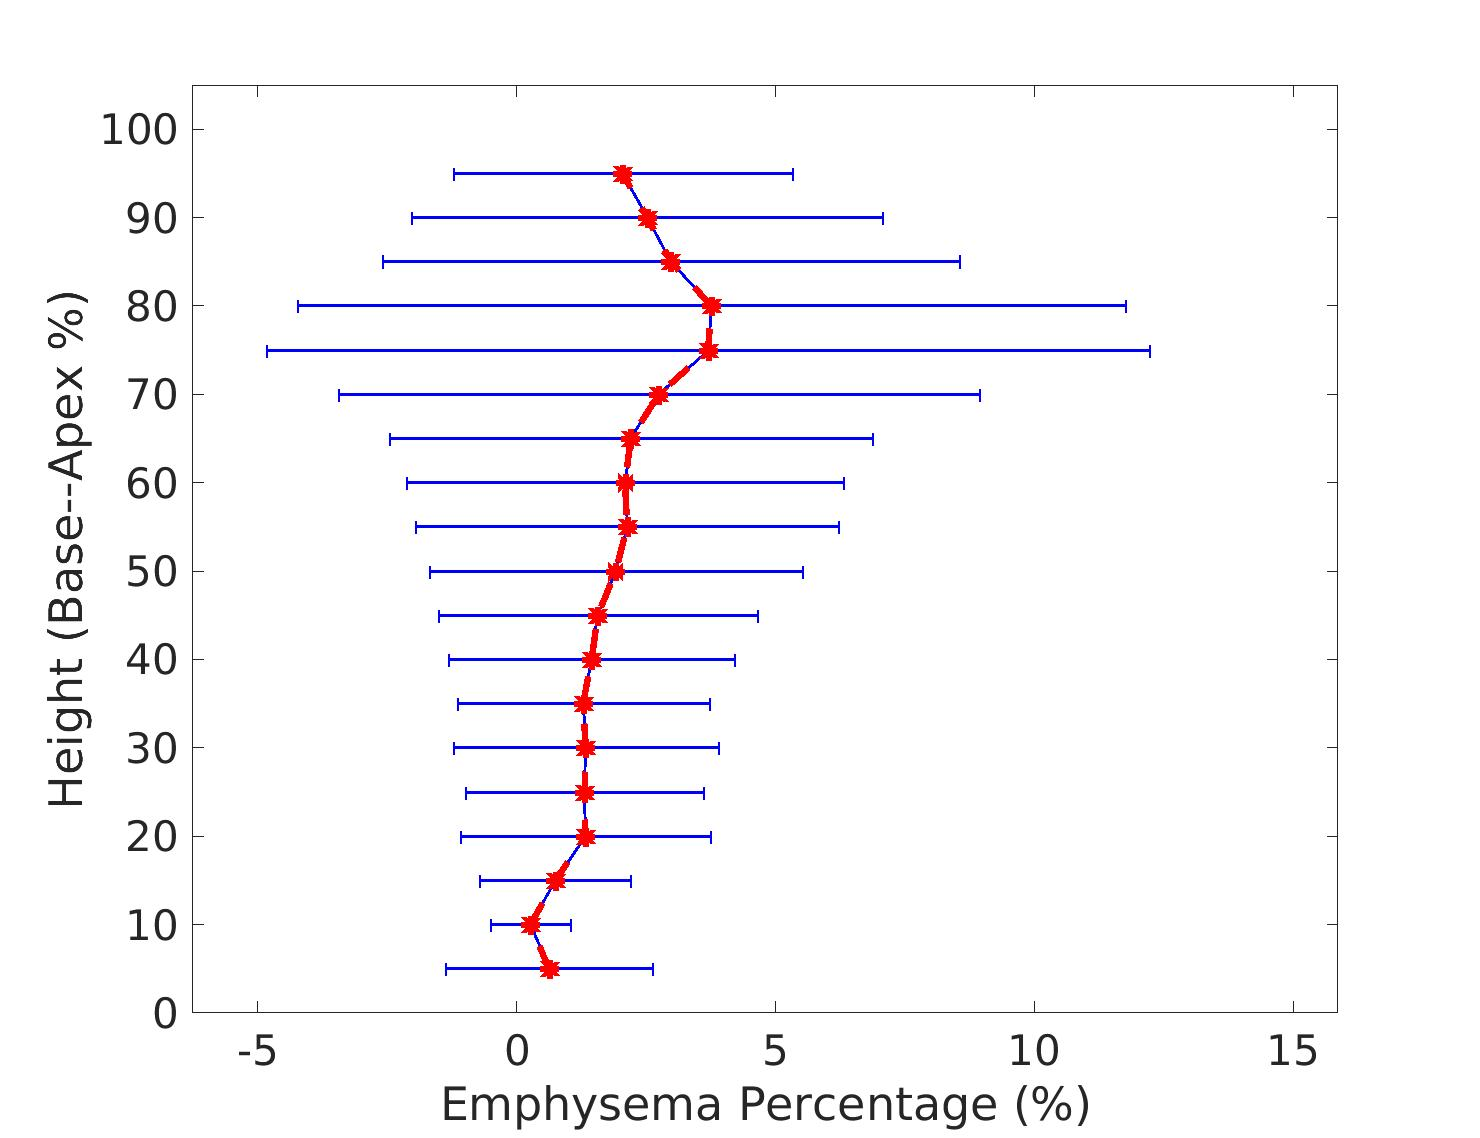
\includegraphics{QuantitativeAnalysis/Image/RightLungEmphysemaDiseaseAgainstHeight.jpg}}
  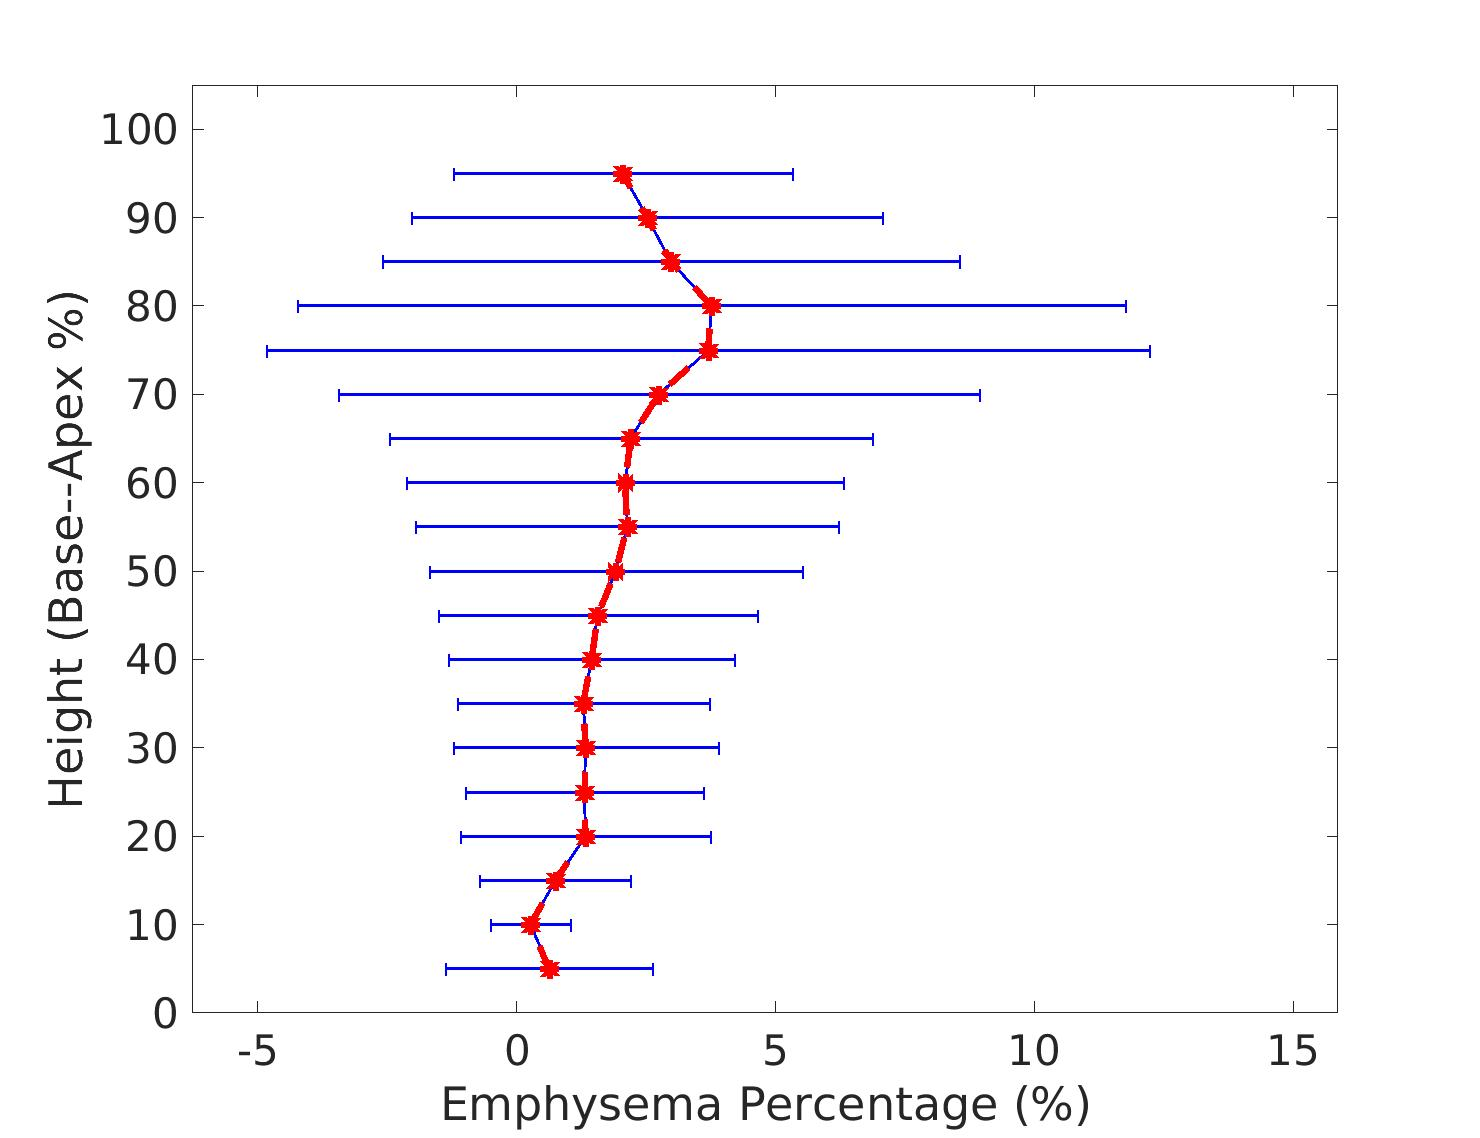
\includegraphics[width=\linewidth,trim={{.0\wd0} {.0\wd0} {.0\wd0} {.0\wd0}},clip]{QuantitativeAnalysis/Image/RightLungEmphysemaDiseaseAgainstHeight.jpg}
  \caption{Right Emphysema}
  \label{fig:DiseaseAgainstHeight-h}
\end{subfigure}
\caption{Volume percentage of each tissue classification plotted against lung height (cranio-caudal axis) in IPF left and right lungs. The average percentage was calculated within 5\% sections of the lung height from the base to apex. Red shows the average value at each position across all patients, and blue shows the standard deviation. (a) (b) is ground-glass distribution. (c) (d) is reticular distribution. (e) (f) is honeycomb distribution. (g) (h) is emphysema distribution.}
\label{fig:DiseaseAgainstHeight}
\end{figure}

\begin{figure}[H] 
\centering
\begin{subfigure}{.42\linewidth}% set image scale
  \sbox0{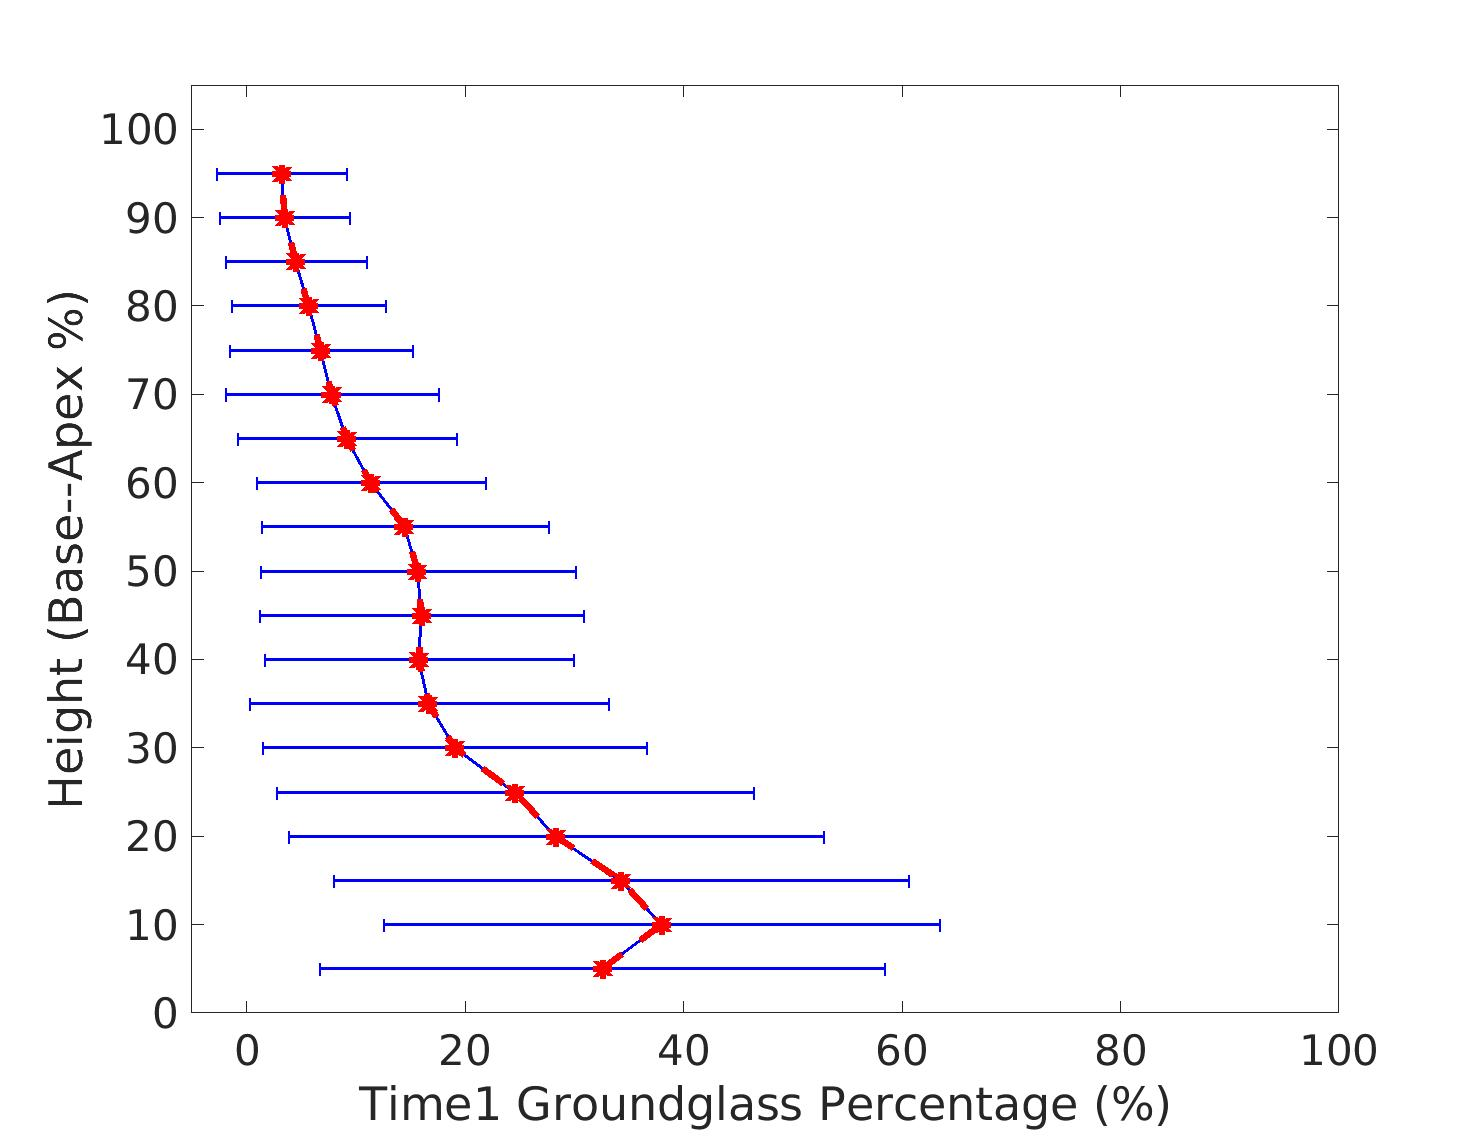
\includegraphics{QuantitativeAnalysis/Image/LeftLungGroundglassDiseaseAgainstHeightTime1.jpg}} 
  %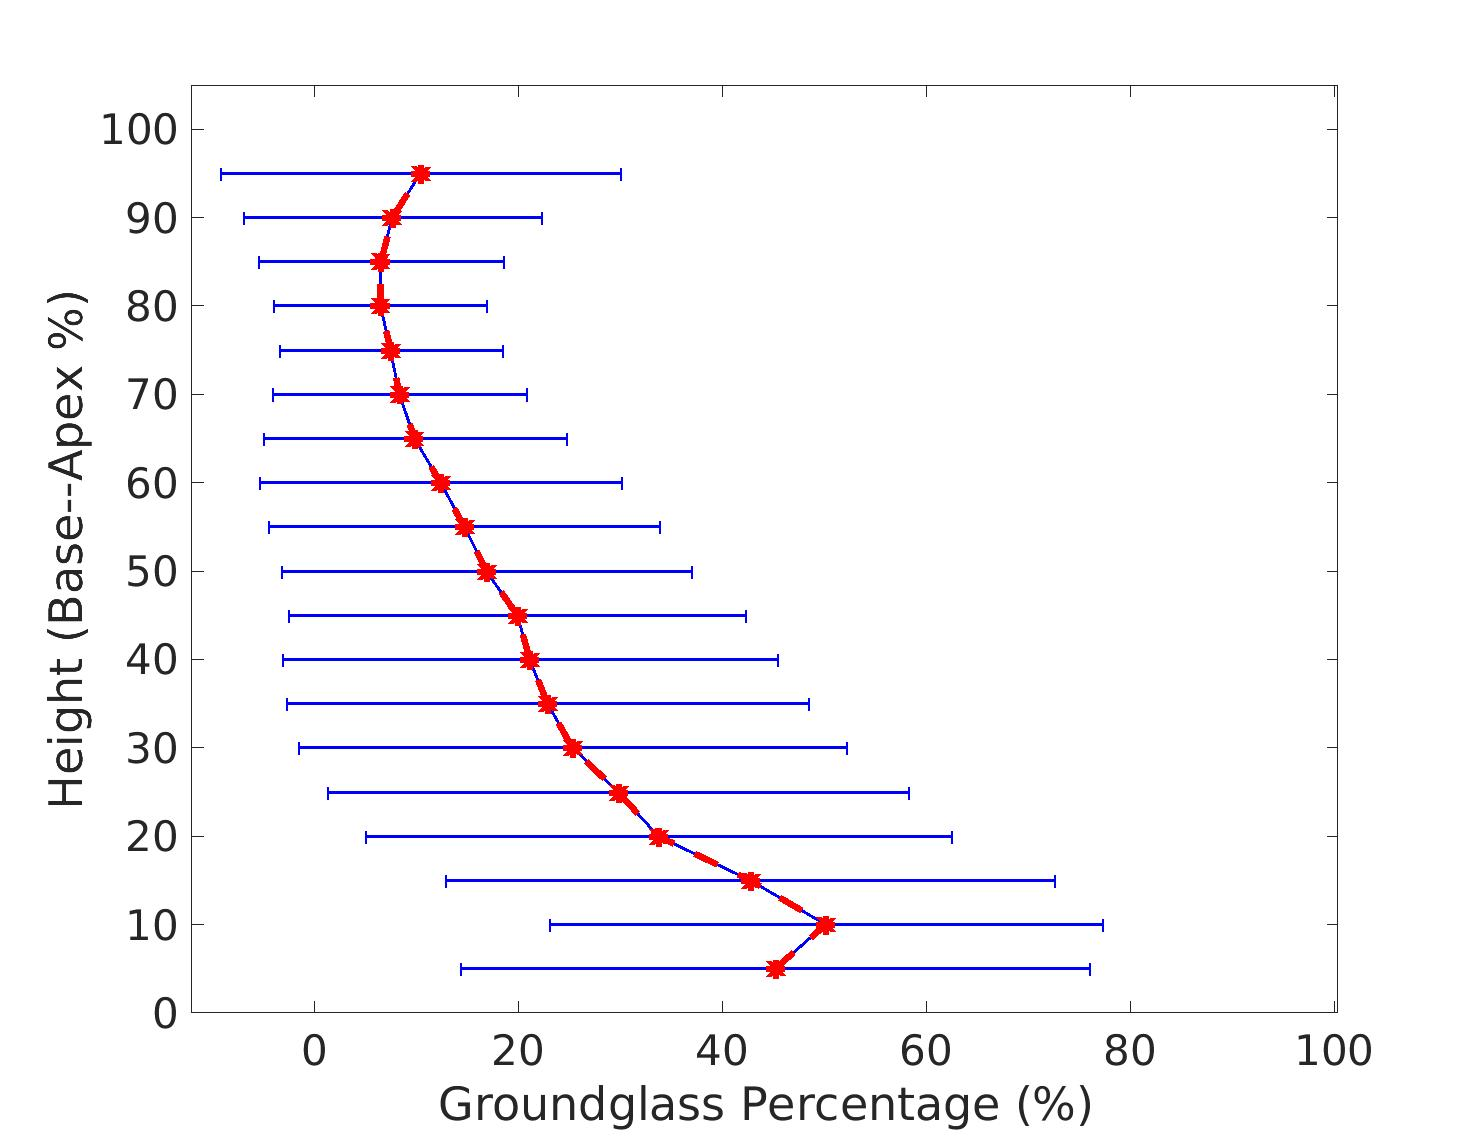
\includegraphics[width=\linewidth,trim={{.0\wd0} {.0\wd0} {.0\wd0} {.0\wd0}},clip]{QuantitativeAnalysis/Image/LeftLungGroundglassDiseaseAgainstHeight.jpg} %trim={<left> <lower> <right> <upper>}, set the cut scale
	\begin{overpic}[width=\linewidth,trim={{.0\wd0} {.0\wd0} {.0\wd0} {.0\wd0}},clip]{QuantitativeAnalysis/Image/LeftLungGroundglassDiseaseAgainstHeightTime1.jpg}
      \put(33,75){\bf{Left lung}}
  \end{overpic}
  \caption{Left ground-glass at month 0}
  \label{fig:DiseaseAgainstHeightTime1-a} 
\end{subfigure} 
\begin{subfigure}{.42\linewidth}% set image scale
  \sbox0{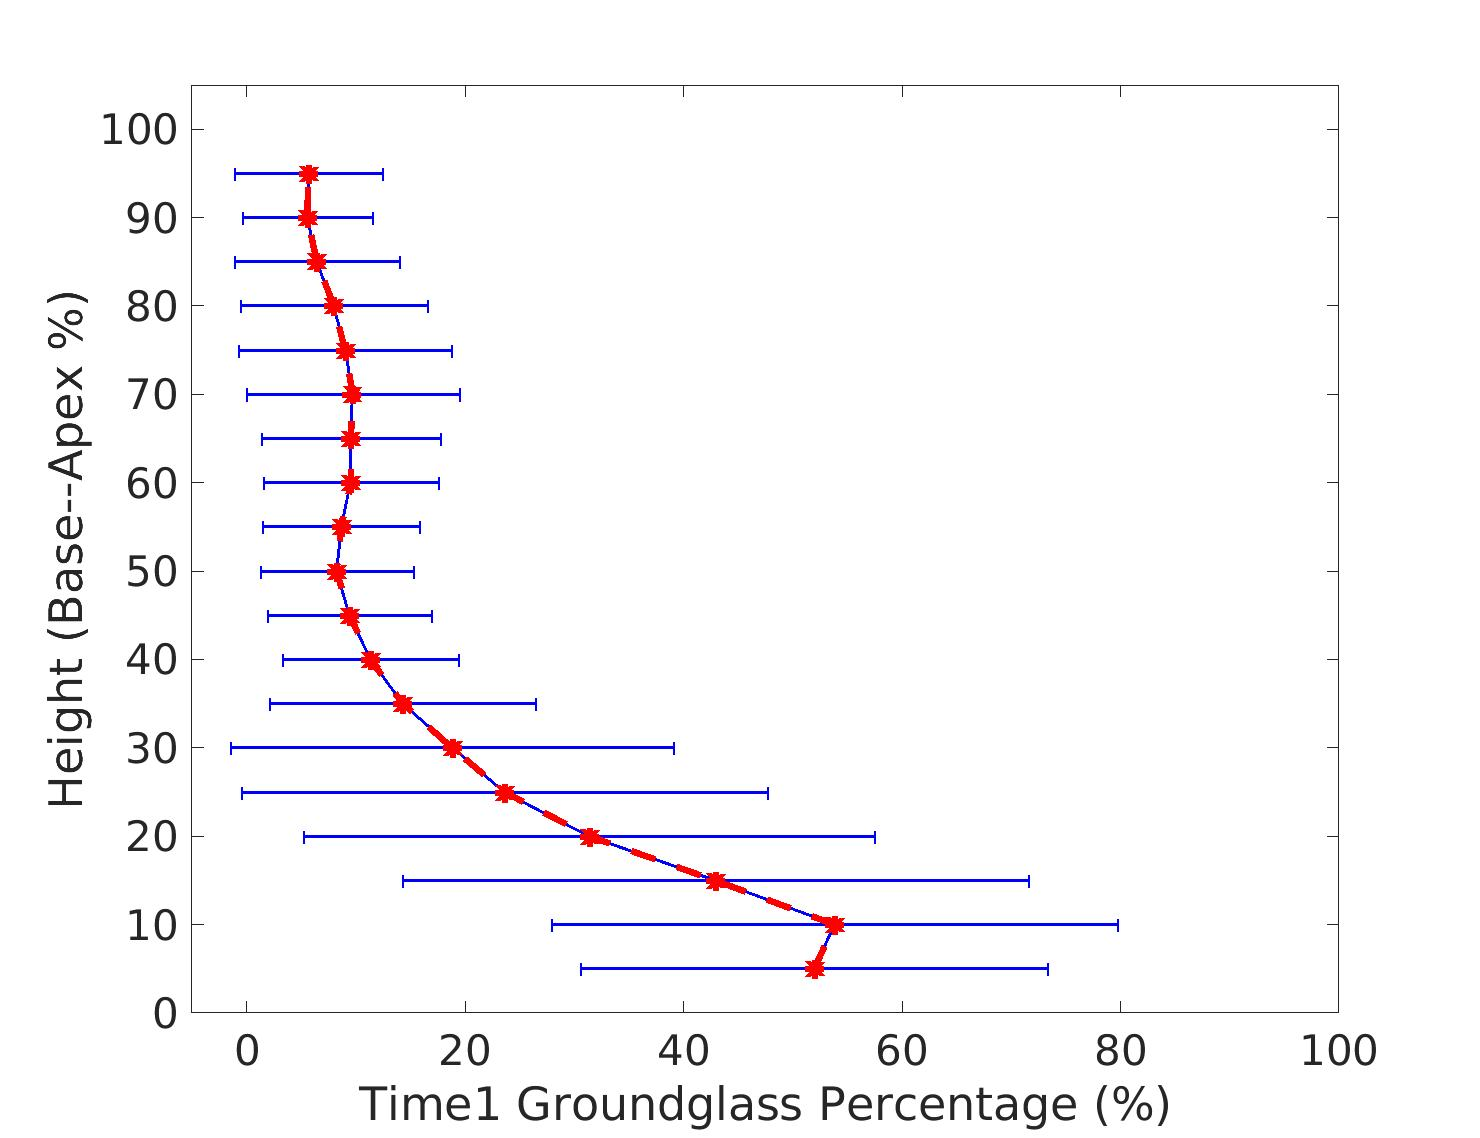
\includegraphics{QuantitativeAnalysis/Image/RightLungGroundglassDiseaseAgainstHeightTime1.jpg}}
  \begin{overpic}[width=\linewidth,trim={{.0\wd0} {.0\wd0} {.0\wd0} {.0\wd0}},clip]{QuantitativeAnalysis/Image/RightLungGroundglassDiseaseAgainstHeightTime1.jpg}
	\put(41,75){\bf{Right lung}}
  \end{overpic}
  \caption{Right ground-glass at month 0}
  \label{fig:DiseaseAgainstHeightTime1-b}
\end{subfigure}
\begin{subfigure}{.42\linewidth}% set image scale
  \sbox0{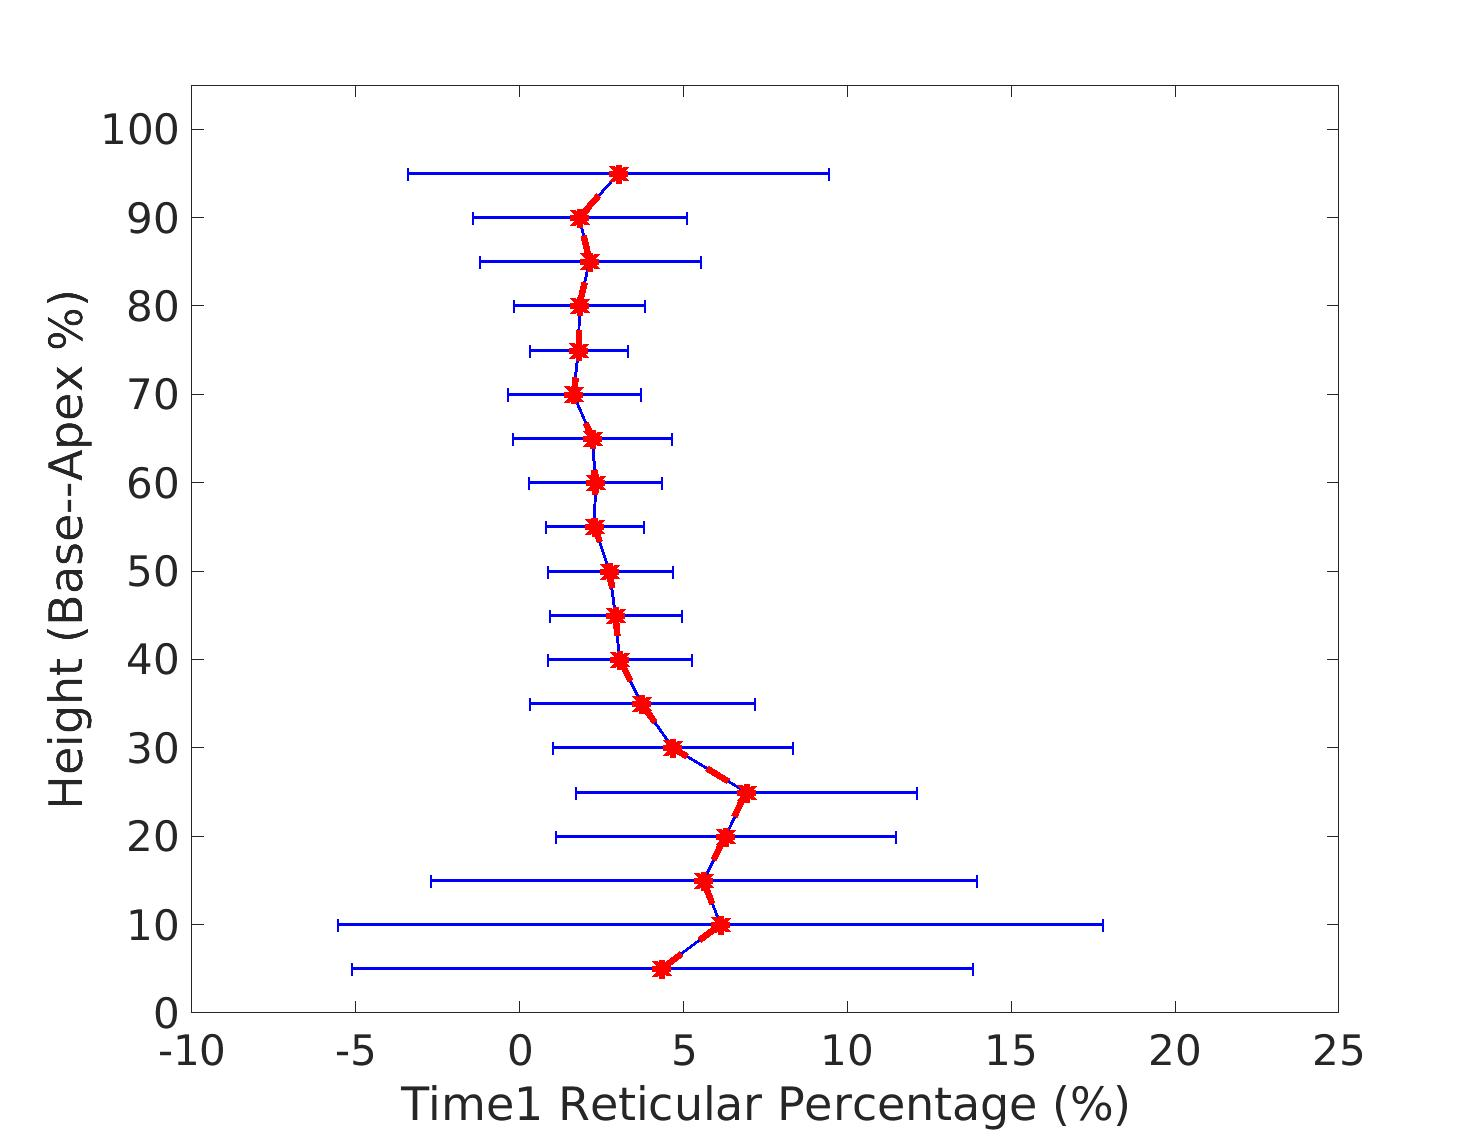
\includegraphics{QuantitativeAnalysis/Image/LeftLungReticularDiseaseAgainstHeightTime1.jpg}} 
  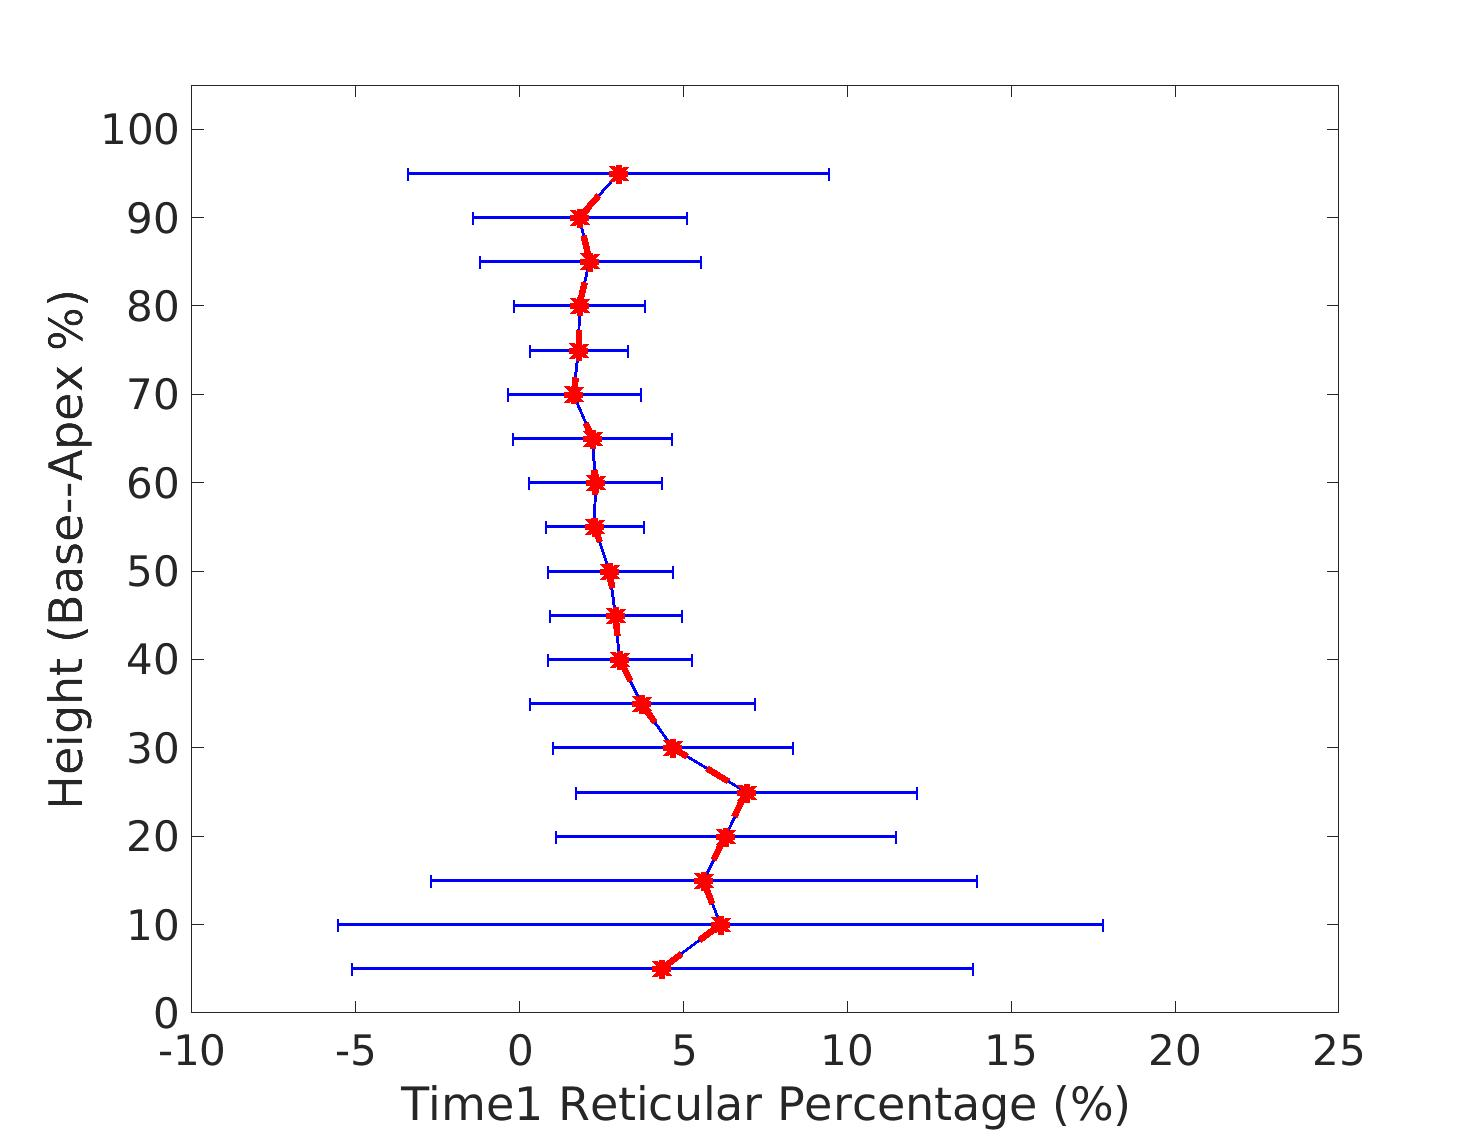
\includegraphics[width=\linewidth,trim={{.0\wd0} {.0\wd0} {.0\wd0} {.0\wd0}},clip]{QuantitativeAnalysis/Image/LeftLungReticularDiseaseAgainstHeightTime1.jpg} %trim={<left> <lower> <right> <upper>}, set the cut scale
  \caption{Left reticular at month 0}
  \label{fig:DiseaseAgainstHeightTime1-c} 
\end{subfigure} 
\begin{subfigure}{.42\linewidth}% set image scale
  \sbox0{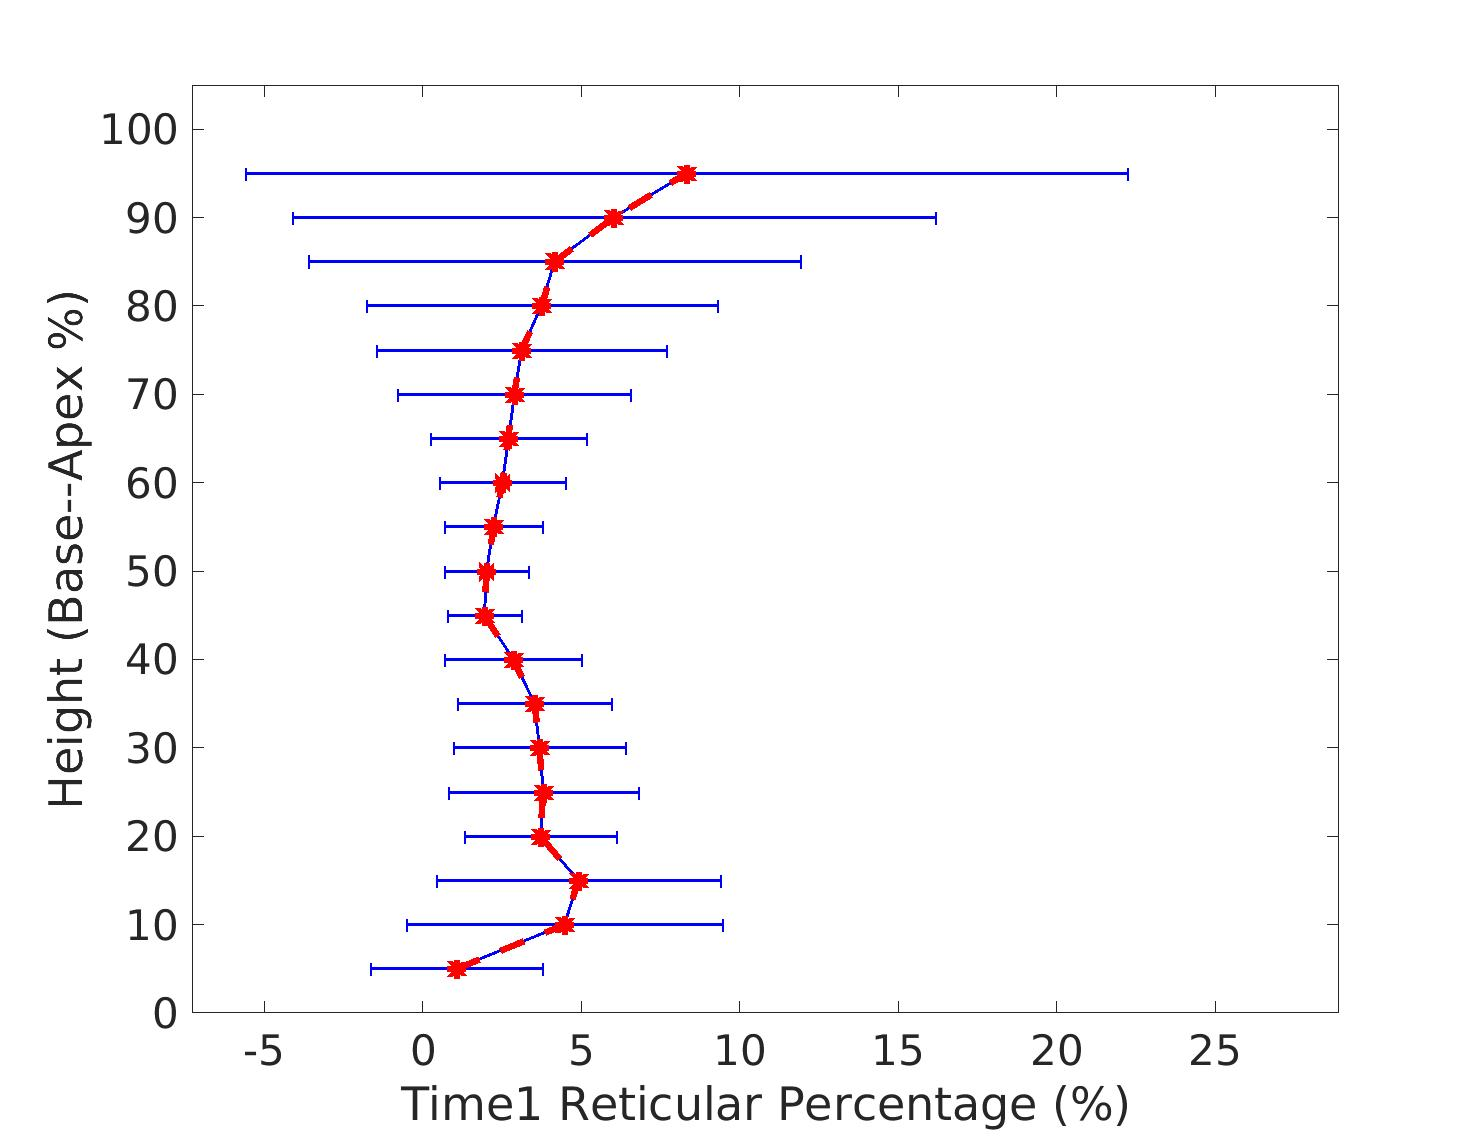
\includegraphics{QuantitativeAnalysis/Image/RightLungReticularDiseaseAgainstHeightTime1.jpg}}
  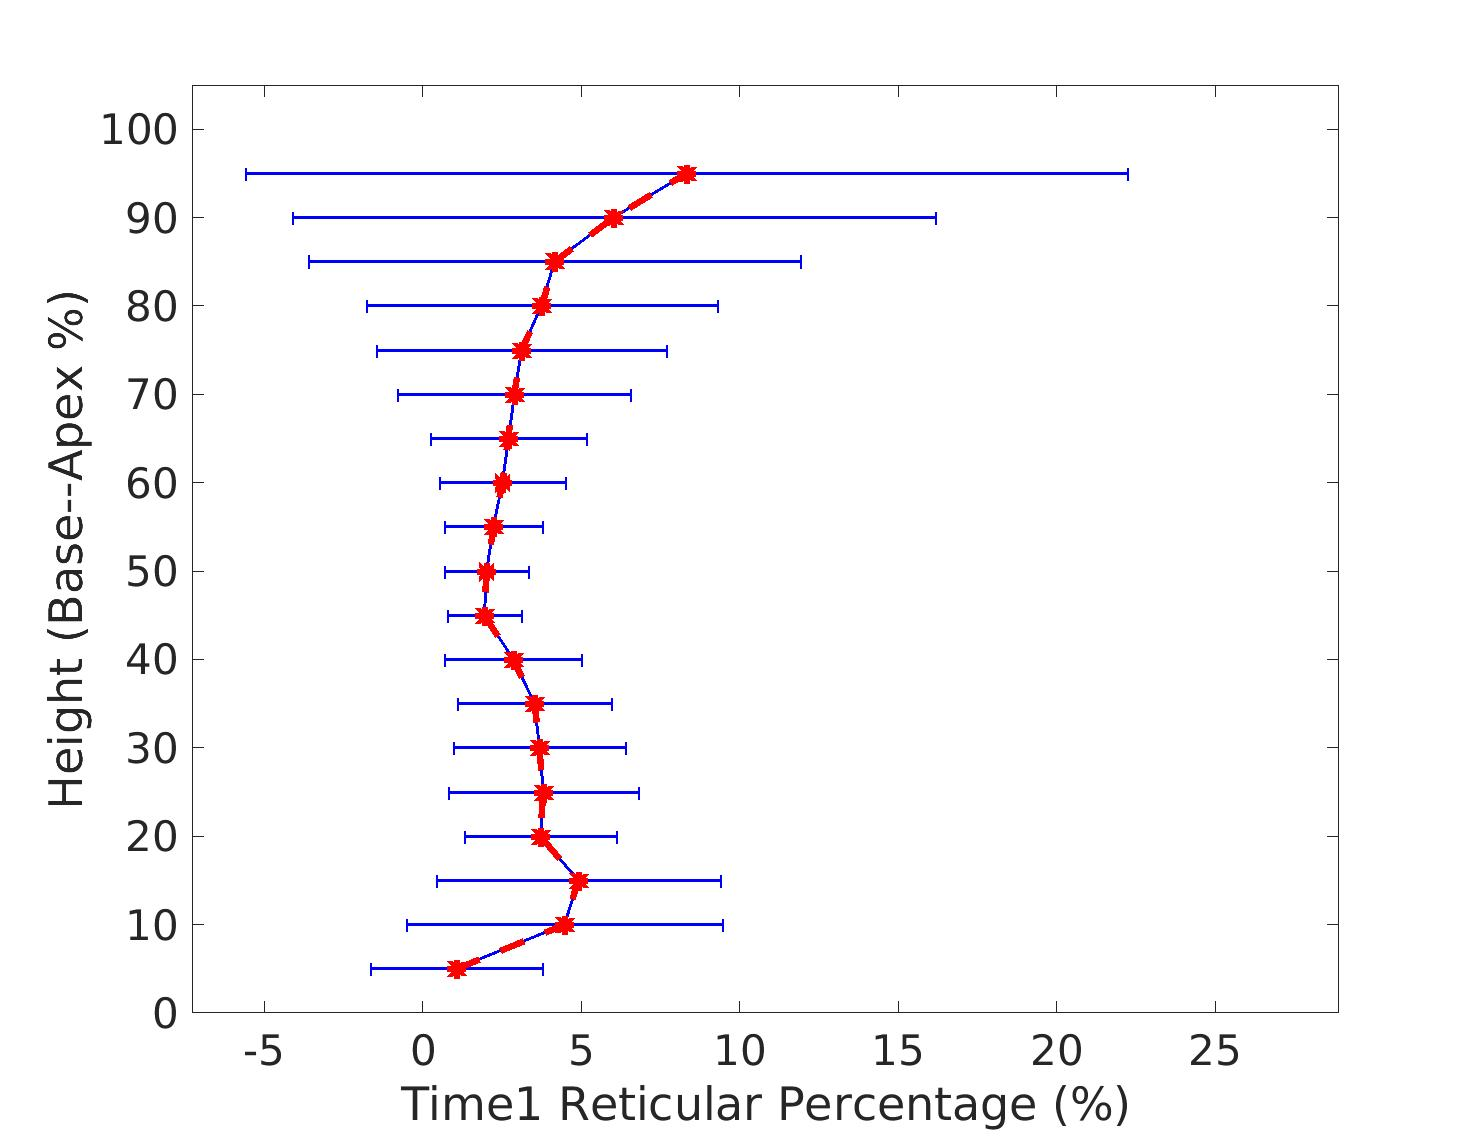
\includegraphics[width=\linewidth,trim={{.0\wd0} {.0\wd0} {.0\wd0} {.0\wd0}},clip]{QuantitativeAnalysis/Image/RightLungReticularDiseaseAgainstHeightTime1.jpg}
  \caption{Right reticular at month 0}
  \label{fig:DiseaseAgainstHeightTime1-d}
\end{subfigure}
\begin{subfigure}{.42\linewidth}% set image scale
  \sbox0{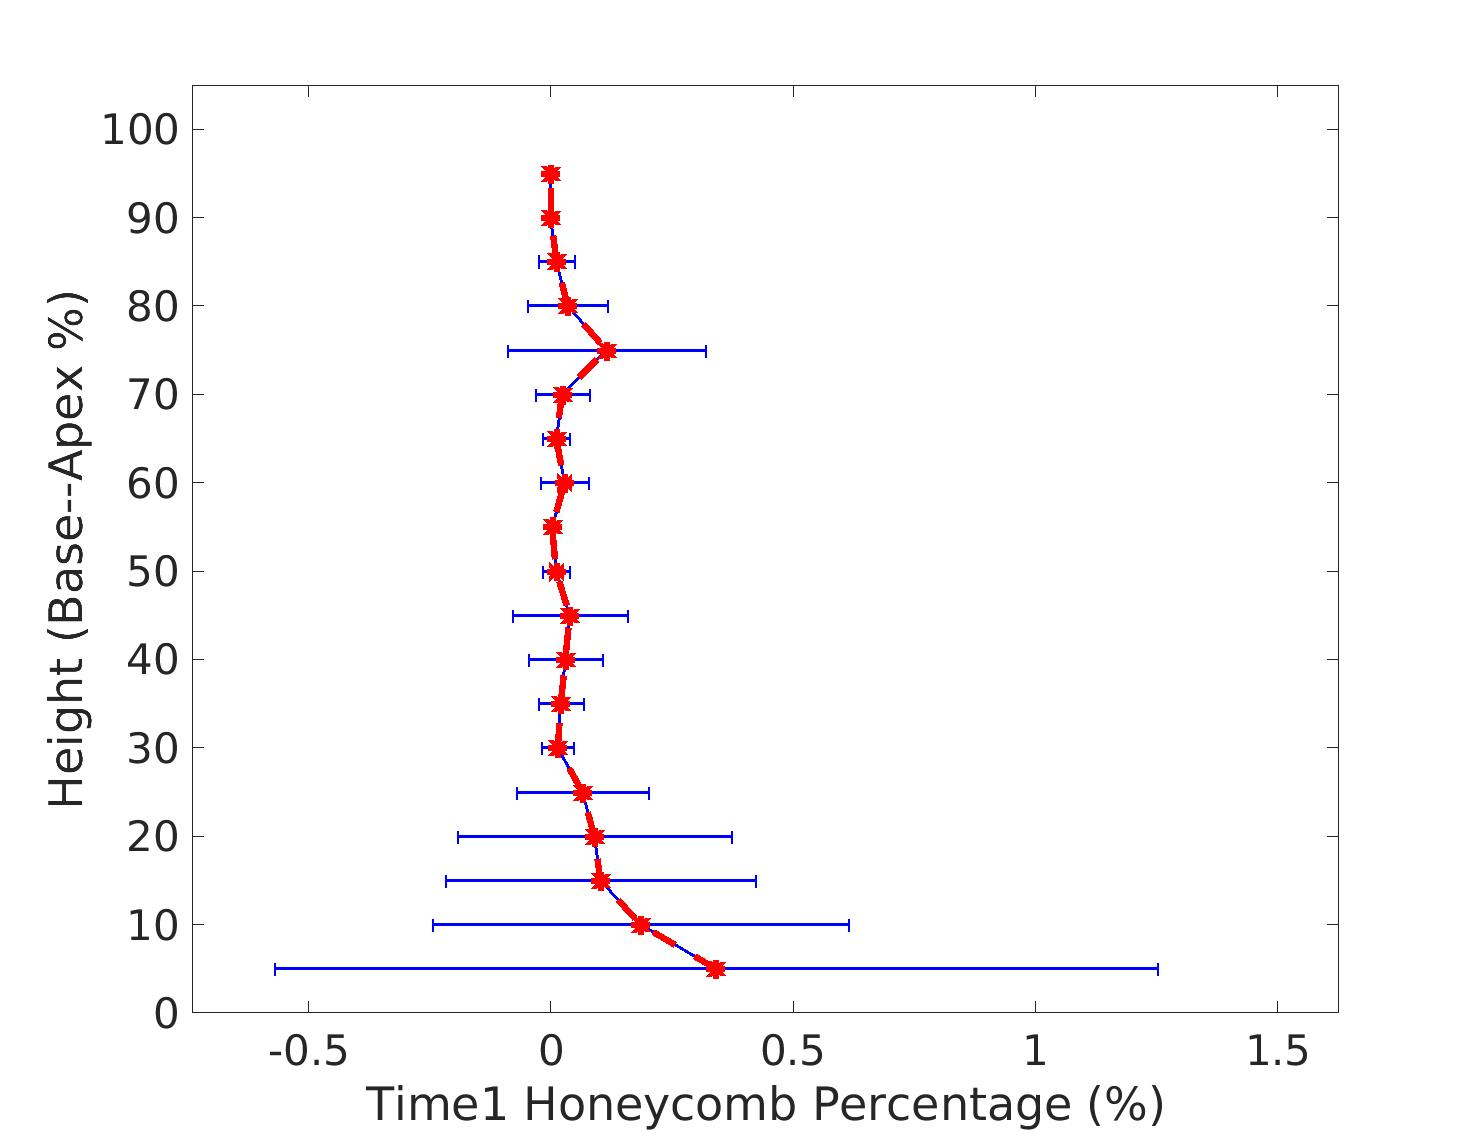
\includegraphics{QuantitativeAnalysis/Image/LeftLungHoneycombDiseaseAgainstHeightTime1.jpg}} 
  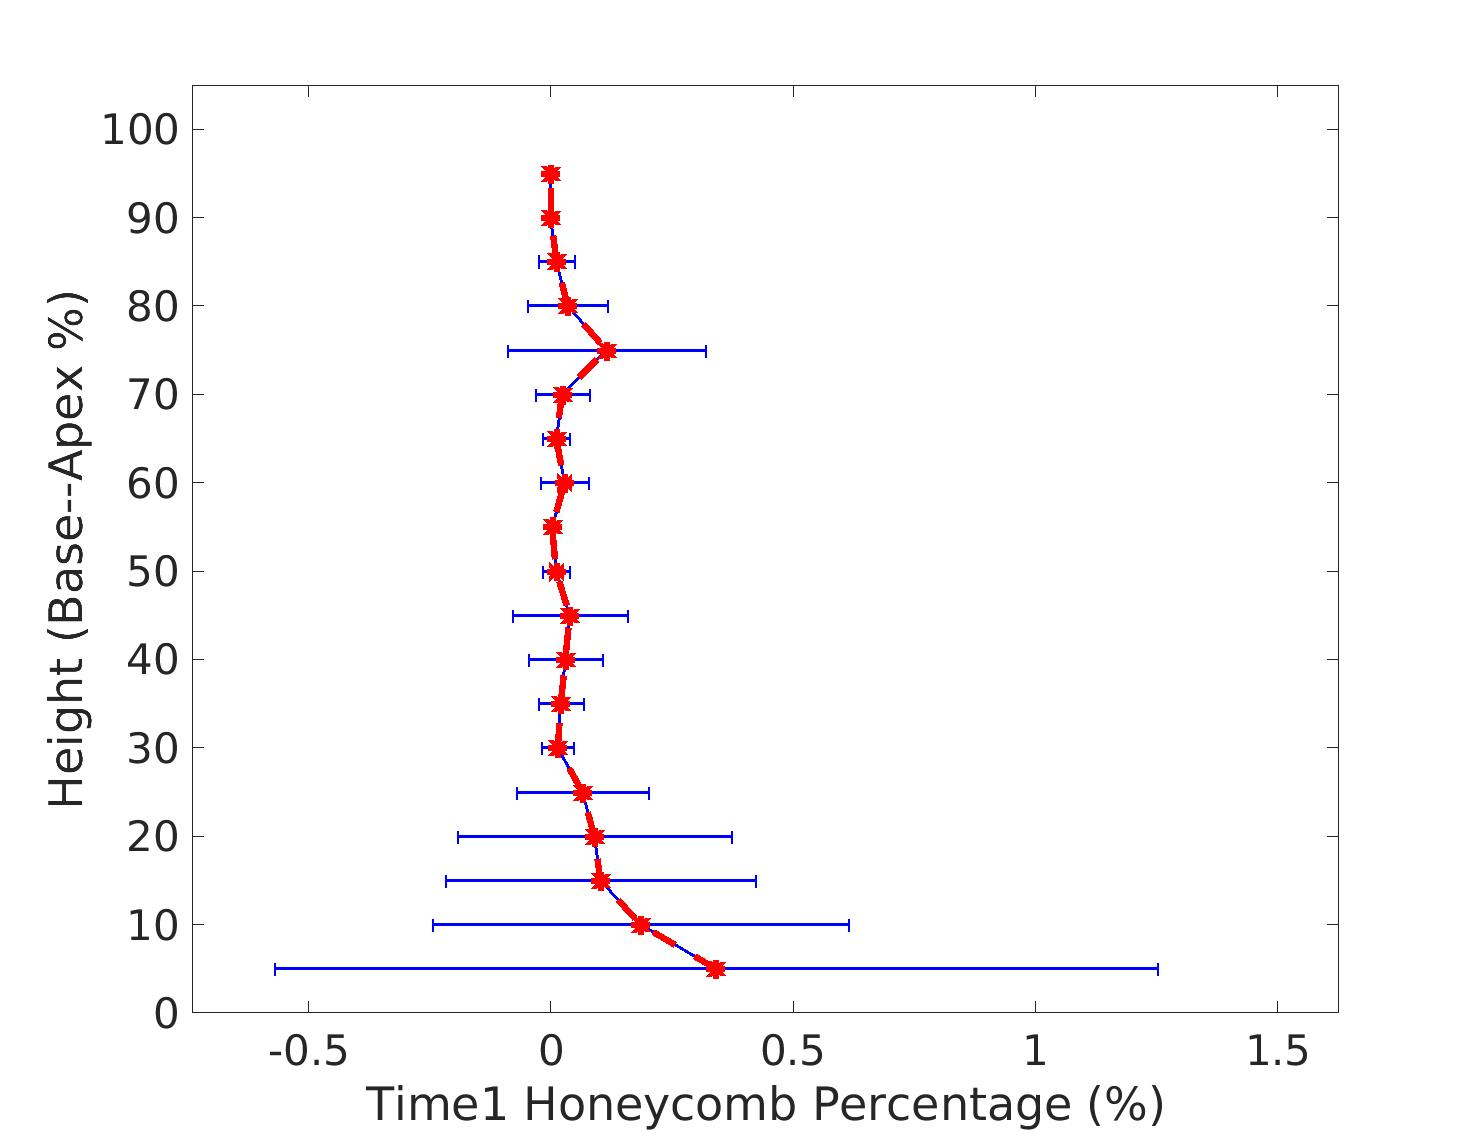
\includegraphics[width=\linewidth,trim={{.0\wd0} {.0\wd0} {.0\wd0} {.0\wd0}},clip]{QuantitativeAnalysis/Image/LeftLungHoneycombDiseaseAgainstHeightTime1.jpg} %trim={<left> <lower> <right> <upper>}, set the cut scale
  \caption{Left honeycomb at month 0}
  \label{fig:DiseaseAgainstHeightTime1-e} 
\end{subfigure} 
\begin{subfigure}{.42\linewidth}% set image scale
  \sbox0{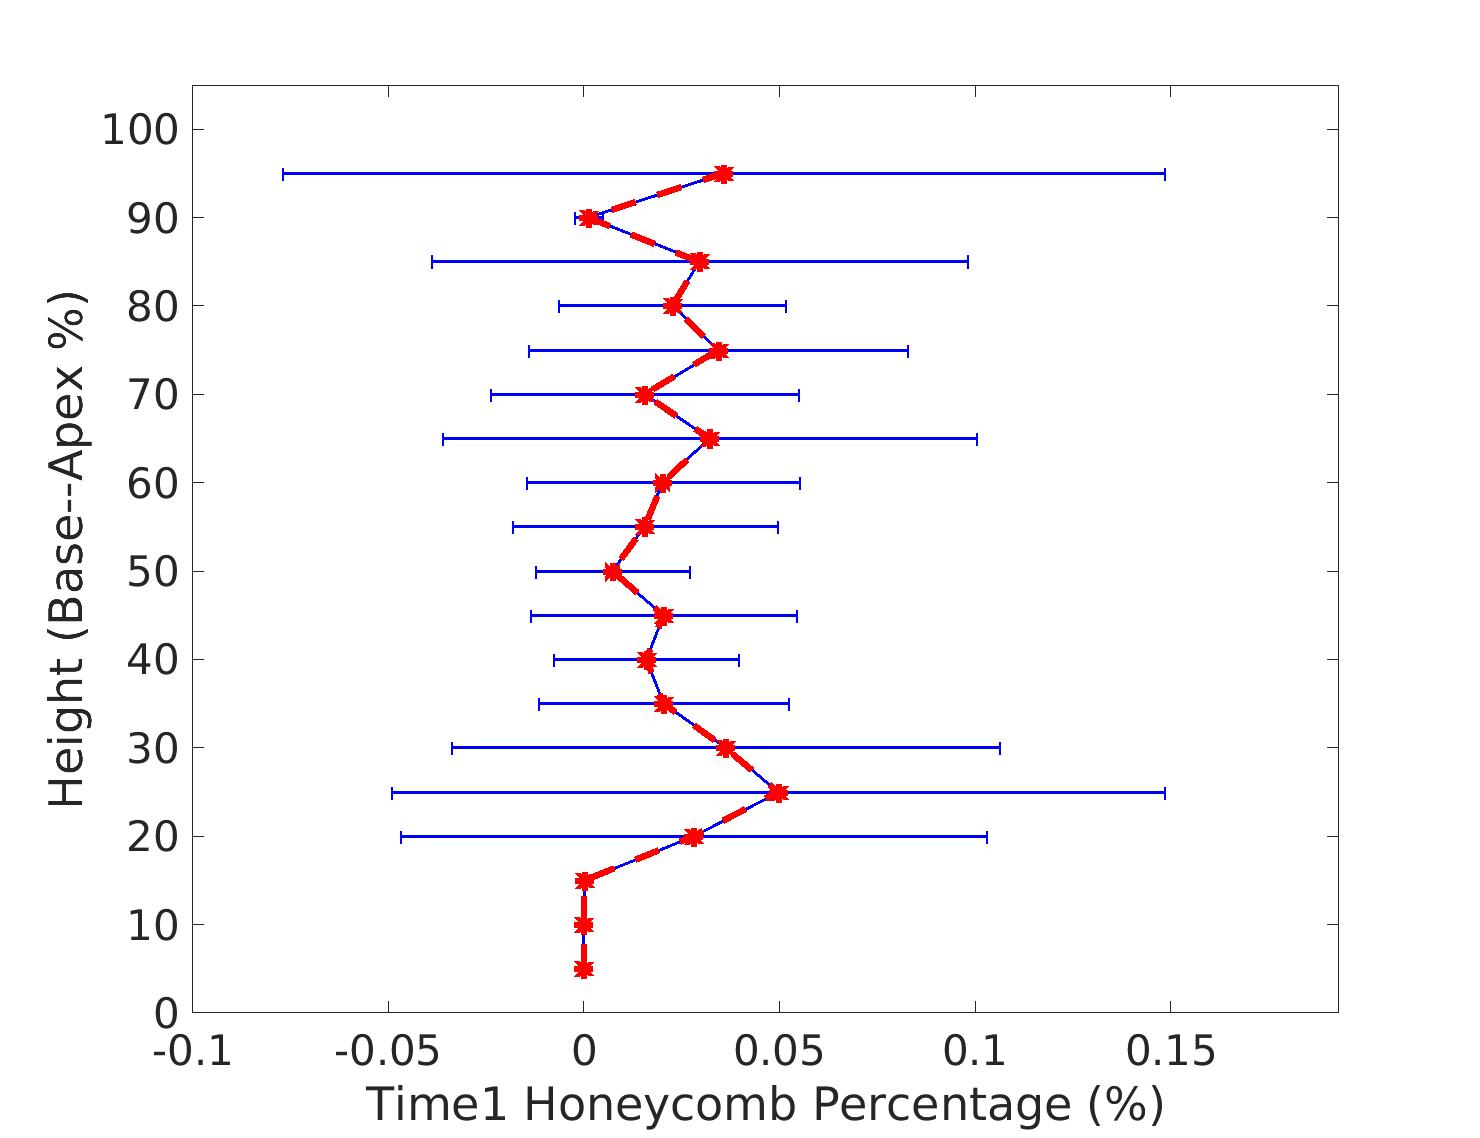
\includegraphics{QuantitativeAnalysis/Image/RightLungHoneycombDiseaseAgainstHeightTime1.jpg}}
  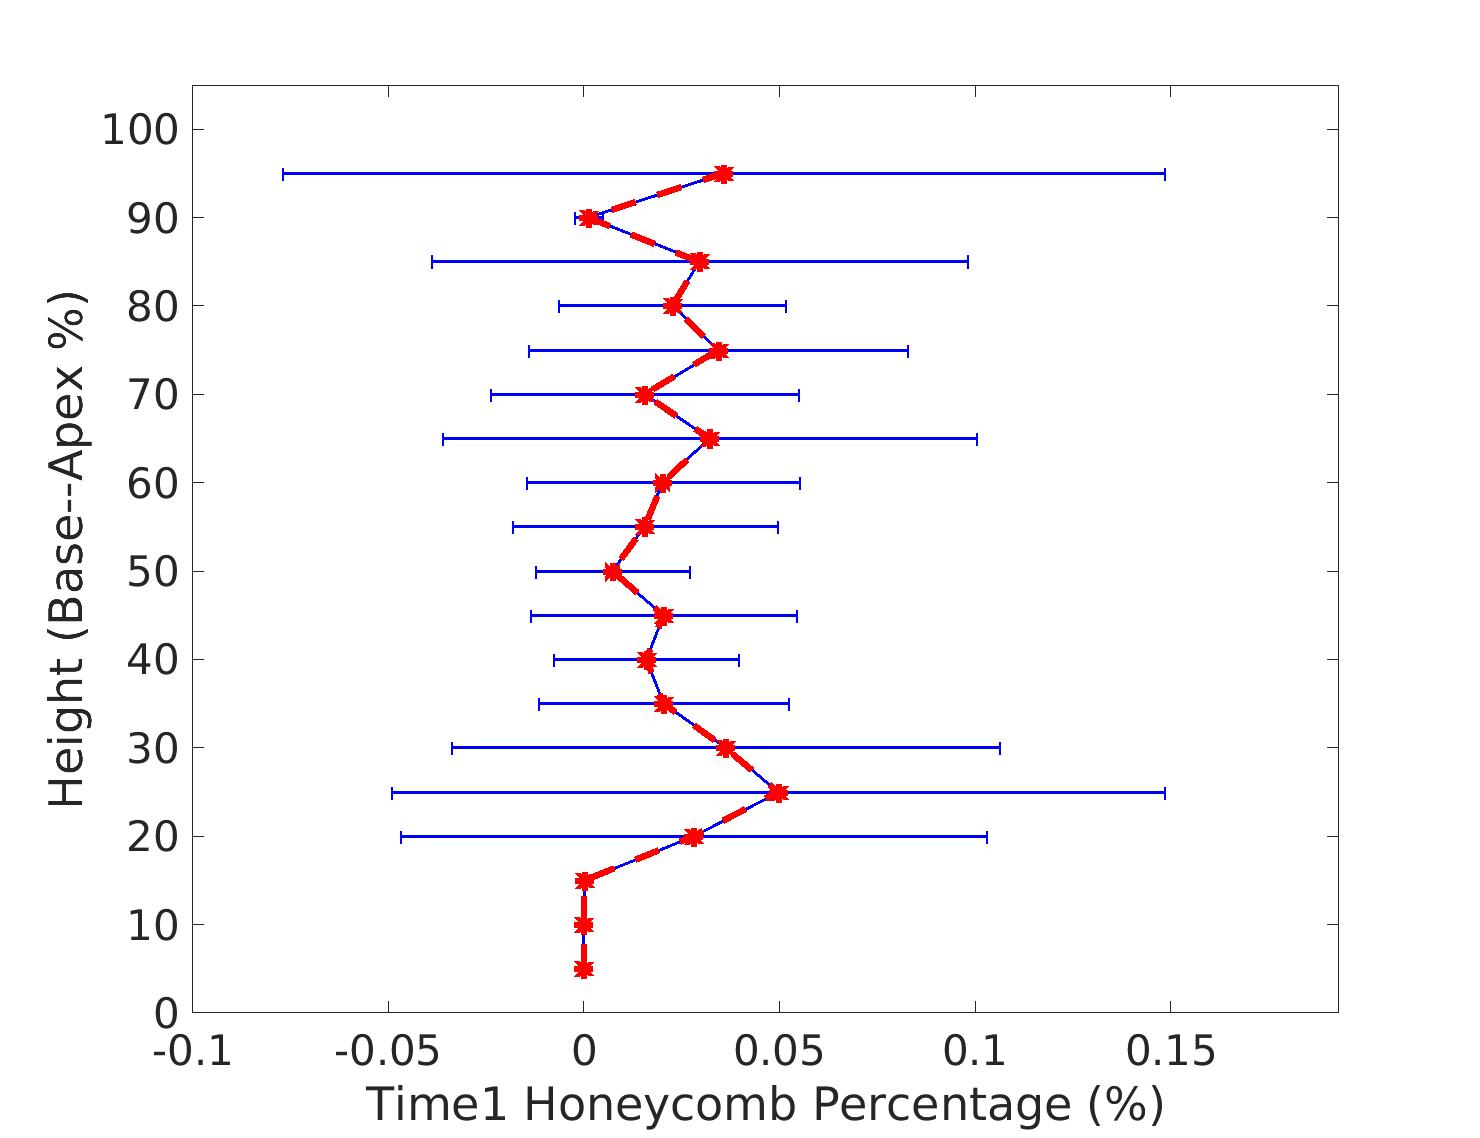
\includegraphics[width=\linewidth,trim={{.0\wd0} {.0\wd0} {.0\wd0} {.0\wd0}},clip]{QuantitativeAnalysis/Image/RightLungHoneycombDiseaseAgainstHeightTime1.jpg}
  \caption{Right honeycomb at month 0}
  \label{fig:DiseaseAgainstHeightTime1-f}
\end{subfigure}
\begin{subfigure}{.42\linewidth}% set image scale
  \sbox0{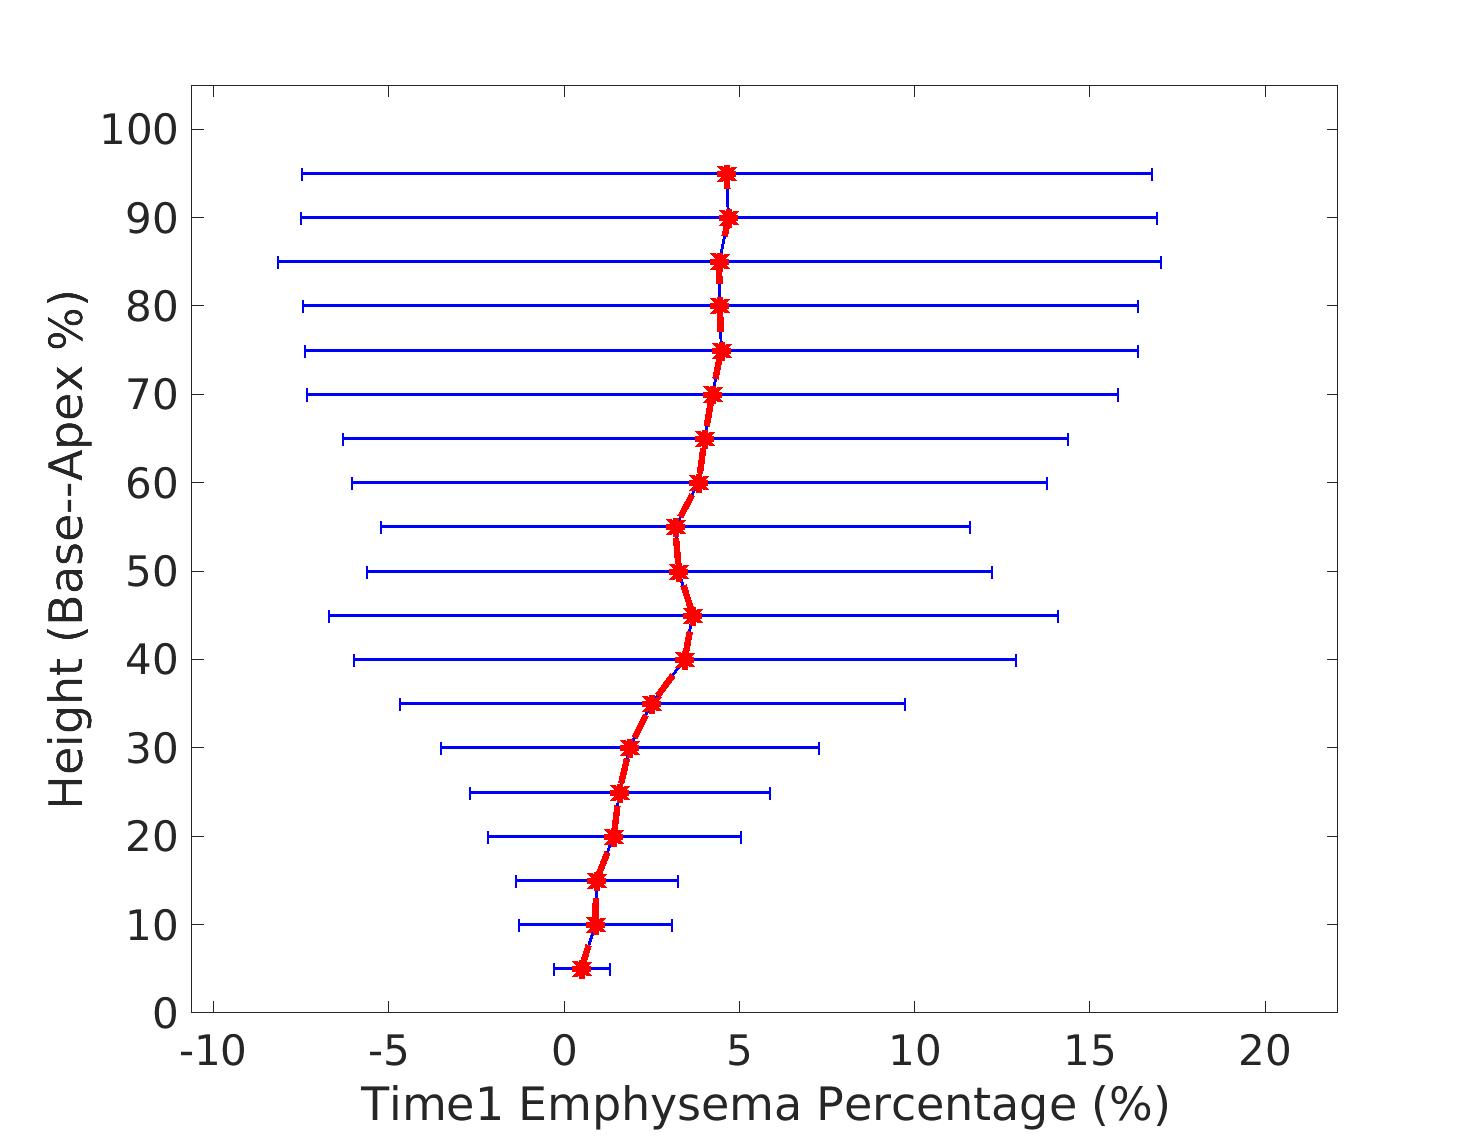
\includegraphics{QuantitativeAnalysis/Image/LeftLungEmphysemaDiseaseAgainstHeightTime1.jpg}} 
  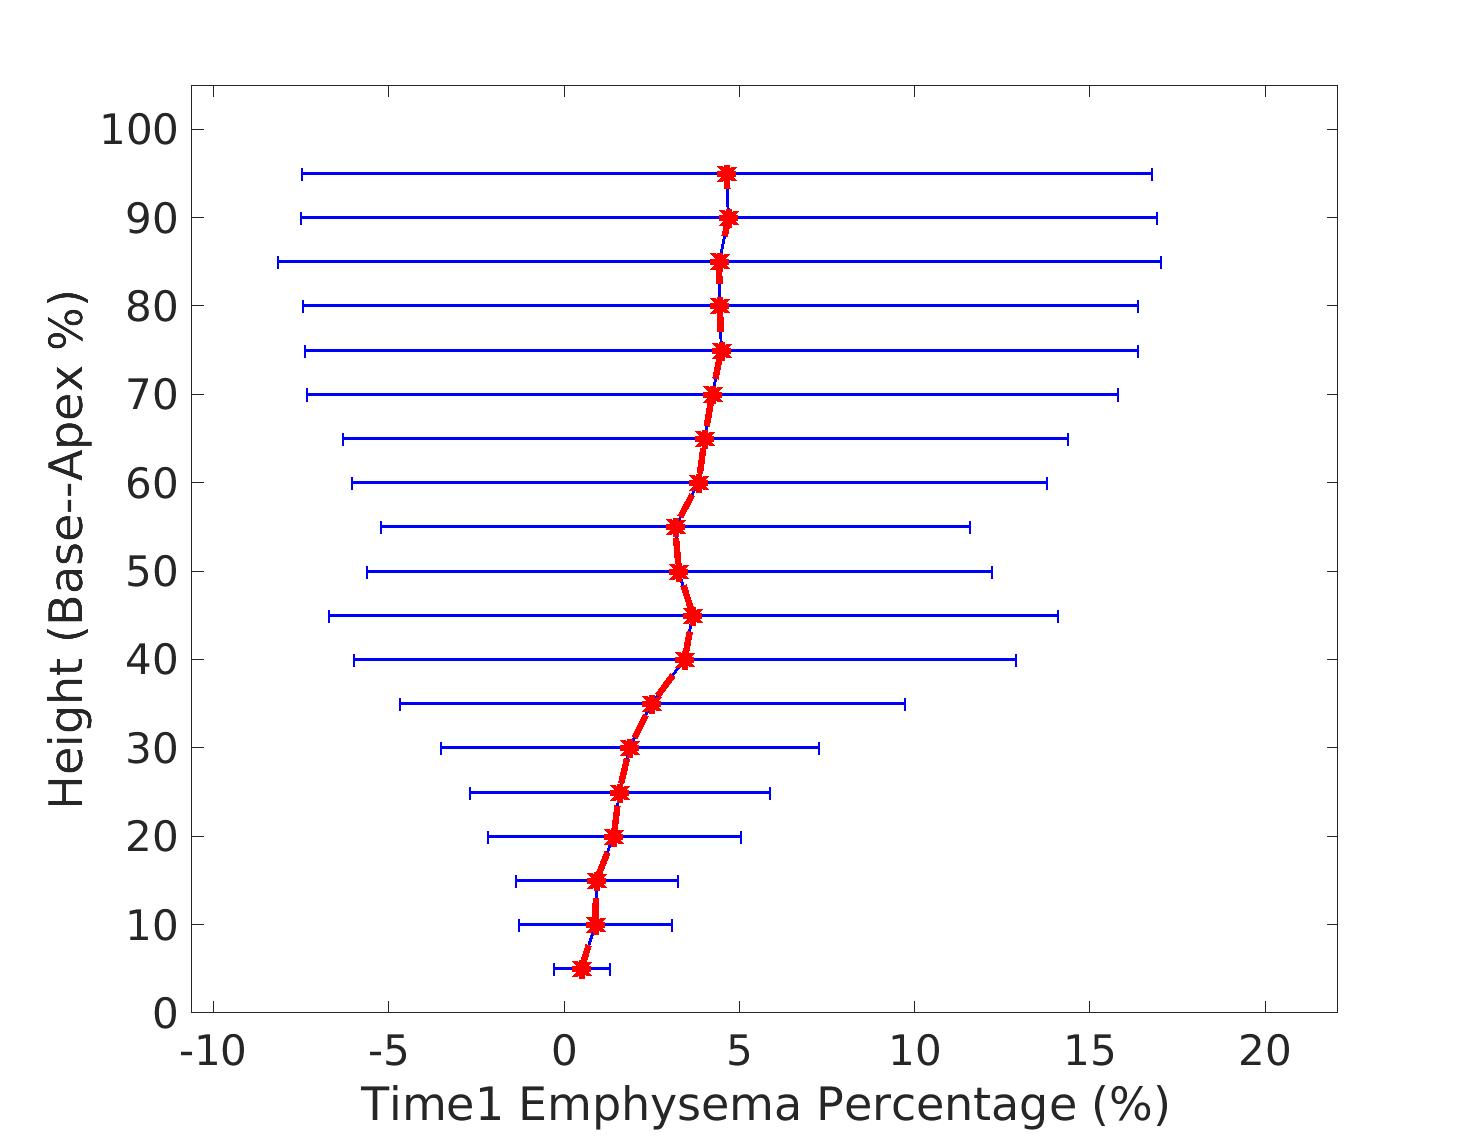
\includegraphics[width=\linewidth,trim={{.0\wd0} {.0\wd0} {.0\wd0} {.0\wd0}},clip]{QuantitativeAnalysis/Image/LeftLungEmphysemaDiseaseAgainstHeightTime1.jpg} %trim={<left> <lower> <right> <upper>}, set the cut scale
  \caption{Left Emphysema at month 0}
  \label{fig:DiseaseAgainstHeightTime1-g} 
\end{subfigure} 
\begin{subfigure}{.42\linewidth}% set image scale
  \sbox0{\includegraphics{QuantitativeAnalysis/Image/RightLungEmphysemaDiseaseAgainstHeightTime1.jpg}}
  \includegraphics[width=\linewidth,trim={{.0\wd0} {.0\wd0} {.0\wd0} {.0\wd0}},clip]{QuantitativeAnalysis/Image/RightLungEmphysemaDiseaseAgainstHeightTime1.jpg}
  \caption{Right Emphysema at month 0}
  \label{fig:DiseaseAgainstHeightTime1-h}
\end{subfigure}
\caption{Volume percentage of each tissue classification plotted against lung height (cranio-caudal axis) in IPF left and right lungs at month 0. The average percentage was calculated within 5\% sections of the lung height from the base to apex. Red shows the average value at each position across all patients, and blue shows the standard deviation. (a) (b) is ground-glass distribution. (c) (d) is reticular distribution. (e) (f) is honeycomb distribution. (g) (h) is emphysema distribution.}
\label{fig:DiseaseAgainstHeightTime1}
\end{figure}

Figure \ref{fig:IPF21DiseaseAgainstHeightMain} shows (for a single representative patient) the percentage distribution against lung height (cranio-caudal axis) of the four characteristic CT patterns in the left and right lung over time. From time point 1 to time point 3, an overall increase of the disease regions can be observed, even though the percentage of some tissue pattern may fall during this time. The distribution of ground-glass and reticular in base-to-apex does not change quantifiably over time, however, there are some fluctuations for honeycomb and emphysema (but the amount of honeycomb is very small). Results are only shown for one representative subject here, because the number of months between imaging is quite variable between subjects which makes it difficult to graphically present the spatial distributions for the entire cohort except for at time 0 or for all time points and subjects simultaneously. The percentage distribution against lung height over time for other patients can be found in Appendix \ref{SpatialDistribution}.
\newpage

\begin{figure}[H] 
\centering
\begin{subfigure}{.42\linewidth}% set image scale
  \sbox0{\includegraphics{QuantitativeAnalysis/Image/IPF21LeftLungGroundglassDiseaseAgainstHeight.jpg}} 
  %\includegraphics[width=\linewidth,trim={{.0\wd0} {.0\wd0} {.0\wd0} {.0\wd0}},clip]{QuantitativeAnalysis/Image/LeftLungGroundglassDiseaseAgainstHeight.jpg} %trim={<left> <lower> <right> <upper>}, set the cut scale
	\begin{overpic}[width=\linewidth,trim={{.0\wd0} {.0\wd0} {.0\wd0} {.0\wd0}},clip]{QuantitativeAnalysis/Image/IPF21LeftLungGroundglassDiseaseAgainstHeight.jpg}
      \put(33,75){\bf{Left lung}}
  \end{overpic}
  \caption{Left ground-glass}
  \label{fig:IPF21DiseaseAgainstHeightMain-a} 
\end{subfigure} 
\begin{subfigure}{.42\linewidth}% set image scale
  \sbox0{\includegraphics{QuantitativeAnalysis/Image/IPF21RightLungGroundglassDiseaseAgainstHeight.jpg}}
  \begin{overpic}[width=\linewidth,trim={{.0\wd0} {.0\wd0} {.0\wd0} {.0\wd0}},clip]{QuantitativeAnalysis/Image/IPF21RightLungGroundglassDiseaseAgainstHeight.jpg}
	\put(41,75){\bf{Right lung}}
  \end{overpic}
  \caption{Right ground-glass}
  \label{fig:IPF21DiseaseAgainstHeightMain-b}
\end{subfigure}
\begin{subfigure}{.42\linewidth}% set image scale
  \sbox0{\includegraphics{QuantitativeAnalysis/Image/IPF21LeftLungReticularDiseaseAgainstHeight.jpg}} 
  \includegraphics[width=\linewidth,trim={{.0\wd0} {.0\wd0} {.0\wd0} {.0\wd0}},clip]{QuantitativeAnalysis/Image/IPF21LeftLungReticularDiseaseAgainstHeight.jpg} %trim={<left> <lower> <right> <upper>}, set the cut scale
  \caption{Left reticular}
  \label{fig:IPF21DiseaseAgainstHeightMain-c} 
\end{subfigure} 
\begin{subfigure}{.42\linewidth}% set image scale
  \sbox0{\includegraphics{QuantitativeAnalysis/Image/IPF21RightLungReticularDiseaseAgainstHeight.jpg}}
  \includegraphics[width=\linewidth,trim={{.0\wd0} {.0\wd0} {.0\wd0} {.0\wd0}},clip]{QuantitativeAnalysis/Image/IPF21RightLungReticularDiseaseAgainstHeight.jpg}
  \caption{Right reticular}
  \label{fig:IPF21DiseaseAgainstHeightMain-d}
\end{subfigure}
\begin{subfigure}{.42\linewidth}% set image scale
  \sbox0{\includegraphics{QuantitativeAnalysis/Image/IPF21LeftLungHoneycombDiseaseAgainstHeight.jpg}} 
  \includegraphics[width=\linewidth,trim={{.0\wd0} {.0\wd0} {.0\wd0} {.0\wd0}},clip]{QuantitativeAnalysis/Image/IPF21LeftLungHoneycombDiseaseAgainstHeight.jpg} %trim={<left> <lower> <right> <upper>}, set the cut scale
  \caption{Left honeycomb}
  \label{fig:IPF21DiseaseAgainstHeightMain-e} 
\end{subfigure} 
\begin{subfigure}{.42\linewidth}% set image scale
  \sbox0{\includegraphics{QuantitativeAnalysis/Image/IPF21RightLungHoneycombDiseaseAgainstHeight.jpg}}
  \includegraphics[width=\linewidth,trim={{.0\wd0} {.0\wd0} {.0\wd0} {.0\wd0}},clip]{QuantitativeAnalysis/Image/IPF21RightLungHoneycombDiseaseAgainstHeight.jpg}
  \caption{Right honeycomb}
  \label{fig:IPF21DiseaseAgainstHeightMain-f}
\end{subfigure}
\begin{subfigure}{.42\linewidth}% set image scale
  \sbox0{\includegraphics{QuantitativeAnalysis/Image/IPF21LeftLungEmphysemaDiseaseAgainstHeight.jpg}} 
  \includegraphics[width=\linewidth,trim={{.0\wd0} {.0\wd0} {.0\wd0} {.0\wd0}},clip]{QuantitativeAnalysis/Image/IPF21LeftLungEmphysemaDiseaseAgainstHeight.jpg} %trim={<left> <lower> <right> <upper>}, set the cut scale
  \caption{Left Emphysema}
  \label{fig:IPF21DiseaseAgainstHeightMain-g} 
\end{subfigure} 
\begin{subfigure}{.42\linewidth}% set image scale
  \sbox0{\includegraphics{QuantitativeAnalysis/Image/IPF21RightLungEmphysemaDiseaseAgainstHeight.jpg}}
  \includegraphics[width=\linewidth,trim={{.0\wd0} {.0\wd0} {.0\wd0} {.0\wd0}},clip]{QuantitativeAnalysis/Image/IPF21RightLungEmphysemaDiseaseAgainstHeight.jpg}
  \caption{Right Emphysema}
  \label{fig:IPF21DiseaseAgainstHeightMain-h}
\end{subfigure}
\caption{Volume percentage of each tissue classification plotted against lung height (cranio-caudal axis) of one patient diagnosed with IPF in left and right lungs over time. The average percentage was calculated within 5\% sections of the lung height from the base to apex. (a) (b) is ground-glass distribution. (c) (d) is reticular distribution. (e) (f) is honeycomb distribution. (g) (h) is emphysema distribution.}
\label{fig:IPF21DiseaseAgainstHeightMain}
\end{figure}

\paragraph{Dorso-to-ventral distribution}
Figure \ref{fig:DiseaseDorsoToVentral} shows the percentage distribution (the average volume percentage of all time points from all patients) from posterior to anterior of the lung (dorso-ventral axis) for the four characteristic CT patterns for left and right lung. The results illustrate that the percentage of ground-glass and reticular keep decreasing from back to front, and they mostly locate in the dorsal part of the left and right lungs. Honeycomb and emphysema are both relatively constant along the dorso-ventral axis, but for the honeycomb pattern, there are relatively more abnormalities appearing in the dorsal and ventral regions compared to the middle area.

Figure \ref{fig:DiseaseDorsoToVentralTime1} shows the percentage distribution (the average volume percentage of the first time point from all patients) from posterior to anterior of the lung (dorso-ventral axis) for the four characteristic CT patterns in left and right lung at month 0. It can be seen that, like the cranio-caudal distribution, the distribution of the diseases in the dorso-ventral direction at the first time point are almost the same as the distribution in Figure \ref{fig:DiseaseDorsoToVentralTime1}, and the disease percentage at month 0 is slightly lower than the total time averaged value.
\newpage

\begin{figure}[H] 
\centering
\begin{subfigure}{.42\linewidth}% set image scale
  \sbox0{\includegraphics{QuantitativeAnalysis/Image/LeftLungGroundglassDiseaseDorsoToVentral.jpg}} 
  %\includegraphics[width=\linewidth,trim={{.0\wd0} {.0\wd0} {.0\wd0} {.0\wd0}},clip]{QuantitativeAnalysis/Image/LeftLungGroundglassDiseaseAgainstHeight.jpg} %trim={<left> <lower> <right> <upper>}, set the cut scale
	\begin{overpic}[width=\linewidth,trim={{.0\wd0} {.0\wd0} {.0\wd0} {.0\wd0}},clip]{QuantitativeAnalysis/Image/LeftLungGroundglassDiseaseDorsoToVentral.jpg}
      \put(33,75){\bf{Left lung}}
  \end{overpic}
  \caption{Left ground-glass}
  \label{fig:DiseaseDorsoToVentral-a} 
\end{subfigure} 
\begin{subfigure}{.42\linewidth}% set image scale
  \sbox0{\includegraphics{QuantitativeAnalysis/Image/RightLungGroundglassDiseaseDorsoToVentral.jpg}}
  \begin{overpic}[width=\linewidth,trim={{.0\wd0} {.0\wd0} {.0\wd0} {.0\wd0}},clip]{QuantitativeAnalysis/Image/RightLungGroundglassDiseaseDorsoToVentral.jpg}
	\put(41,75){\bf{Right lung}}
  \end{overpic}
  \caption{Right ground-glass}
  \label{fig:DiseaseDorsoToVentral-b}
\end{subfigure}
\begin{subfigure}{.42\linewidth}% set image scale
  \sbox0{\includegraphics{QuantitativeAnalysis/Image/LeftLungReticularDiseaseDorsoToVentral.jpg}} 
  \includegraphics[width=\linewidth,trim={{.0\wd0} {.0\wd0} {.0\wd0} {.0\wd0}},clip]{QuantitativeAnalysis/Image/LeftLungReticularDiseaseDorsoToVentral.jpg} %trim={<left> <lower> <right> <upper>}, set the cut scale
  \caption{Left reticular}
  \label{fig:DiseaseDorsoToVentral-c} 
\end{subfigure} 
\begin{subfigure}{.42\linewidth}% set image scale
  \sbox0{\includegraphics{QuantitativeAnalysis/Image/RightLungReticularDiseaseDorsoToVentral.jpg}}
  \includegraphics[width=\linewidth,trim={{.0\wd0} {.0\wd0} {.0\wd0} {.0\wd0}},clip]{QuantitativeAnalysis/Image/RightLungReticularDiseaseDorsoToVentral.jpg}
  \caption{Right reticular}
  \label{fig:DiseaseDorsoToVentral-d}
\end{subfigure}
\begin{subfigure}{.42\linewidth}% set image scale
  \sbox0{\includegraphics{QuantitativeAnalysis/Image/LeftLungHoneycombDiseaseDorsoToVentral.jpg}} 
  \includegraphics[width=\linewidth,trim={{.0\wd0} {.0\wd0} {.0\wd0} {.0\wd0}},clip]{QuantitativeAnalysis/Image/LeftLungHoneycombDiseaseDorsoToVentral.jpg} %trim={<left> <lower> <right> <upper>}, set the cut scale
  \caption{Left honeycomb}
  \label{fig:DiseaseDorsoToVentral-e} 
\end{subfigure} 
\begin{subfigure}{.42\linewidth}% set image scale
  \sbox0{\includegraphics{QuantitativeAnalysis/Image/RightLungHoneycombDiseaseDorsoToVentral.jpg}}
  \includegraphics[width=\linewidth,trim={{.0\wd0} {.0\wd0} {.0\wd0} {.0\wd0}},clip]{QuantitativeAnalysis/Image/RightLungHoneycombDiseaseDorsoToVentral.jpg}
  \caption{Right honeycomb}
  \label{fig:DiseaseDorsoToVentral-f}
\end{subfigure}
\begin{subfigure}{.42\linewidth}% set image scale
  \sbox0{\includegraphics{QuantitativeAnalysis/Image/LeftLungEmphysemaDiseaseDorsoToVentral.jpg}} 
  \includegraphics[width=\linewidth,trim={{.0\wd0} {.0\wd0} {.0\wd0} {.0\wd0}},clip]{QuantitativeAnalysis/Image/LeftLungEmphysemaDiseaseDorsoToVentral.jpg} %trim={<left> <lower> <right> <upper>}, set the cut scale
  \caption{Left Emphysema}
  \label{fig:DiseaseDorsoToVentral-g} 
\end{subfigure} 
\begin{subfigure}{.42\linewidth}% set image scale
  \sbox0{\includegraphics{QuantitativeAnalysis/Image/RightLungEmphysemaDiseaseDorsoToVentral.jpg}}
  \includegraphics[width=\linewidth,trim={{.0\wd0} {.0\wd0} {.0\wd0} {.0\wd0}},clip]{QuantitativeAnalysis/Image/RightLungEmphysemaDiseaseDorsoToVentral.jpg}
  \caption{Right Emphysema}
  \label{fig:DiseaseDorsoToVentral-h}
\end{subfigure}
\caption{Volume percentage of each tissue classification plotted in the direction of dorso-ventral axis in IPF left and right lungs. The average percentage was calculated within 5\% sections along the axis from posterior to anterior. Red shows the average value at each position across all patients, and blue shows the standard deviation. (a) (b) is ground-glass distribution. (c) (d) is reticular distribution. (e) (f) is honeycomb distribution. (g) (h) is emphysema distribution.}
\label{fig:DiseaseDorsoToVentral}
\end{figure}

\begin{figure}[H] 
\centering
\begin{subfigure}{.42\linewidth}% set image scale
  \sbox0{\includegraphics{QuantitativeAnalysis/Image/LeftLungGroundglassDiseaseDorsoToVentralTime1.jpg}} 
  %\includegraphics[width=\linewidth,trim={{.0\wd0} {.0\wd0} {.0\wd0} {.0\wd0}},clip]{QuantitativeAnalysis/Image/LeftLungGroundglassDiseaseAgainstHeight.jpg} %trim={<left> <lower> <right> <upper>}, set the cut scale
	\begin{overpic}[width=\linewidth,trim={{.0\wd0} {.0\wd0} {.0\wd0} {.0\wd0}},clip]{QuantitativeAnalysis/Image/LeftLungGroundglassDiseaseDorsoToVentralTime1.jpg}
      \put(33,75){\bf{Left lung}}
  \end{overpic}
  \caption{Left ground-glass at month 0}
  \label{fig:DiseaseDorsoToVentralTime1-a} 
\end{subfigure} 
\begin{subfigure}{.42\linewidth}% set image scale
  \sbox0{\includegraphics{QuantitativeAnalysis/Image/RightLungGroundglassDiseaseDorsoToVentralTime1.jpg}}
  \begin{overpic}[width=\linewidth,trim={{.0\wd0} {.0\wd0} {.0\wd0} {.0\wd0}},clip]{QuantitativeAnalysis/Image/RightLungGroundglassDiseaseDorsoToVentralTime1.jpg}
	\put(41,75){\bf{Right lung}}
  \end{overpic}
  \caption{Right ground-glass at month 0}
  \label{fig:DiseaseDorsoToVentralTime1-b}
\end{subfigure}
\begin{subfigure}{.42\linewidth}% set image scale
  \sbox0{\includegraphics{QuantitativeAnalysis/Image/LeftLungReticularDiseaseDorsoToVentralTime1.jpg}} 
  \includegraphics[width=\linewidth,trim={{.0\wd0} {.0\wd0} {.0\wd0} {.0\wd0}},clip]{QuantitativeAnalysis/Image/LeftLungReticularDiseaseDorsoToVentralTime1.jpg} %trim={<left> <lower> <right> <upper>}, set the cut scale
  \caption{Left reticular at month 0}
  \label{fig:DiseaseDorsoToVentralTime1-c} 
\end{subfigure} 
\begin{subfigure}{.42\linewidth}% set image scale
  \sbox0{\includegraphics{QuantitativeAnalysis/Image/RightLungReticularDiseaseDorsoToVentralTime1.jpg}}
  \includegraphics[width=\linewidth,trim={{.0\wd0} {.0\wd0} {.0\wd0} {.0\wd0}},clip]{QuantitativeAnalysis/Image/RightLungReticularDiseaseDorsoToVentralTime1.jpg}
  \caption{Right reticular at month 0}
  \label{fig:DiseaseDorsoToVentralTime1-d}
\end{subfigure}
\begin{subfigure}{.42\linewidth}% set image scale
  \sbox0{\includegraphics{QuantitativeAnalysis/Image/LeftLungHoneycombDiseaseDorsoToVentralTime1.jpg}} 
  \includegraphics[width=\linewidth,trim={{.0\wd0} {.0\wd0} {.0\wd0} {.0\wd0}},clip]{QuantitativeAnalysis/Image/LeftLungHoneycombDiseaseDorsoToVentralTime1.jpg} %trim={<left> <lower> <right> <upper>}, set the cut scale
  \caption{Left honeycomb at month 0}
  \label{fig:DiseaseDorsoToVentralTime1-e} 
\end{subfigure} 
\begin{subfigure}{.42\linewidth}% set image scale
  \sbox0{\includegraphics{QuantitativeAnalysis/Image/RightLungHoneycombDiseaseDorsoToVentralTime1.jpg}}
  \includegraphics[width=\linewidth,trim={{.0\wd0} {.0\wd0} {.0\wd0} {.0\wd0}},clip]{QuantitativeAnalysis/Image/RightLungHoneycombDiseaseDorsoToVentralTime1.jpg}
  \caption{Right honeycomb at month 0}
  \label{fig:DiseaseDorsoToVentralTime1-f}
\end{subfigure}
\begin{subfigure}{.42\linewidth}% set image scale
  \sbox0{\includegraphics{QuantitativeAnalysis/Image/LeftLungEmphysemaDiseaseDorsoToVentralTime1.jpg}} 
  \includegraphics[width=\linewidth,trim={{.0\wd0} {.0\wd0} {.0\wd0} {.0\wd0}},clip]{QuantitativeAnalysis/Image/LeftLungEmphysemaDiseaseDorsoToVentralTime1.jpg} %trim={<left> <lower> <right> <upper>}, set the cut scale
  \caption{Left Emphysema at month 0}
  \label{fig:DiseaseDorsoToVentralTime1-g} 
\end{subfigure} 
\begin{subfigure}{.42\linewidth}% set image scale
  \sbox0{\includegraphics{QuantitativeAnalysis/Image/RightLungEmphysemaDiseaseDorsoToVentralTime1.jpg}}
  \includegraphics[width=\linewidth,trim={{.0\wd0} {.0\wd0} {.0\wd0} {.0\wd0}},clip]{QuantitativeAnalysis/Image/RightLungEmphysemaDiseaseDorsoToVentralTime1.jpg}
  \caption{Right Emphysema at month 0}
  \label{fig:DiseaseDorsoToVentralTime1-h}
\end{subfigure}
\caption{Volume percentage of each tissue classification plotted in the direction of the dorso-ventral axis in IPF left and right lungs at month 0. The average percentage was calculated within 5\% sections along the axis from posterior to anterior. Red shows the average value at each position across all patients, and blue shows the standard deviation. (a) (b) is ground-glass distribution. (c) (d) is reticular distribution. (e) (f) is honeycomb distribution. (g) (h) is emphysema distribution.}
\label{fig:DiseaseDorsoToVentralTime1}
\end{figure}

Figure \ref{fig:IPF21DiseaseDorsoToVentralMain} shows the percentage distribution from the posterior to anterior of the lung (dorso-ventral axis) of the four characteristic CT patterns from an individual patient diagnosed with IPF in left and right lung over time. For ground-glass, emphysema and left honeycomb, an increase in the volume percentage over time can be seen and the dorso-ventral distribution does not change quantifiably during this period of time. However, the spatial location of reticular and honeycomb (in the right lungs) redistributes in the dorso-ventral direction over time, and no consistent trend is observed. The percentage distribution in this axis over time for all patients can be found in Appendix \ref{SpatialDistribution}.
\newpage

\begin{figure}[H] 
\centering
\begin{subfigure}{.42\linewidth}% set image scale
  \sbox0{\includegraphics{QuantitativeAnalysis/Image/IPF21LeftLungGroundglassDiseaseDorsoToVentral.jpg}} 
  %\includegraphics[width=\linewidth,trim={{.0\wd0} {.0\wd0} {.0\wd0} {.0\wd0}},clip]{QuantitativeAnalysis/Image/LeftLungGroundglassDiseaseAgainstHeight.jpg} %trim={<left> <lower> <right> <upper>}, set the cut scale
	\begin{overpic}[width=\linewidth,trim={{.0\wd0} {.0\wd0} {.0\wd0} {.0\wd0}},clip]{QuantitativeAnalysis/Image/IPF21LeftLungGroundglassDiseaseDorsoToVentral.jpg}
      \put(33,75){\bf{Left lung}}
  \end{overpic}
  \caption{Left ground-glass}
  \label{fig:IPF21DiseaseDorsoToVentralMain-a} 
\end{subfigure} 
\begin{subfigure}{.42\linewidth}% set image scale
  \sbox0{\includegraphics{QuantitativeAnalysis/Image/IPF21RightLungGroundglassDiseaseDorsoToVentral.jpg}}
  \begin{overpic}[width=\linewidth,trim={{.0\wd0} {.0\wd0} {.0\wd0} {.0\wd0}},clip]{QuantitativeAnalysis/Image/IPF21RightLungGroundglassDiseaseDorsoToVentral.jpg}
	\put(41,75){\bf{Right lung}}
  \end{overpic}
  \caption{Right ground-glass}
  \label{fig:IPF21DiseaseDorsoToVentralMain-b}
\end{subfigure}
\begin{subfigure}{.42\linewidth}% set image scale
  \sbox0{\includegraphics{QuantitativeAnalysis/Image/IPF21LeftLungReticularDiseaseDorsoToVentral.jpg}} 
  \includegraphics[width=\linewidth,trim={{.0\wd0} {.0\wd0} {.0\wd0} {.0\wd0}},clip]{QuantitativeAnalysis/Image/IPF21LeftLungReticularDiseaseDorsoToVentral.jpg} %trim={<left> <lower> <right> <upper>}, set the cut scale
  \caption{Left reticular}
  \label{fig:IPF21DiseaseDorsoToVentralMain-c} 
\end{subfigure} 
\begin{subfigure}{.42\linewidth}% set image scale
  \sbox0{\includegraphics{QuantitativeAnalysis/Image/IPF21RightLungReticularDiseaseDorsoToVentral.jpg}}
  \includegraphics[width=\linewidth,trim={{.0\wd0} {.0\wd0} {.0\wd0} {.0\wd0}},clip]{QuantitativeAnalysis/Image/IPF21RightLungReticularDiseaseDorsoToVentral.jpg}
  \caption{Right reticular}
  \label{fig:IPF21DiseaseDorsoToVentralMain-d}
\end{subfigure}
\begin{subfigure}{.42\linewidth}% set image scale
  \sbox0{\includegraphics{QuantitativeAnalysis/Image/IPF21LeftLungHoneycombDiseaseDorsoToVentral.jpg}} 
  \includegraphics[width=\linewidth,trim={{.0\wd0} {.0\wd0} {.0\wd0} {.0\wd0}},clip]{QuantitativeAnalysis/Image/IPF21LeftLungHoneycombDiseaseDorsoToVentral.jpg} %trim={<left> <lower> <right> <upper>}, set the cut scale
  \caption{Left honeycomb}
  \label{fig:IPF21DiseaseDorsoToVentralMain-e} 
\end{subfigure} 
\begin{subfigure}{.42\linewidth}% set image scale
  \sbox0{\includegraphics{QuantitativeAnalysis/Image/IPF21RightLungHoneycombDiseaseDorsoToVentral.jpg}}
  \includegraphics[width=\linewidth,trim={{.0\wd0} {.0\wd0} {.0\wd0} {.0\wd0}},clip]{QuantitativeAnalysis/Image/IPF21RightLungHoneycombDiseaseDorsoToVentral.jpg}
  \caption{Right honeycomb}
  \label{fig:IPF21DiseaseDorsoToVentralMain-f}
\end{subfigure}
\begin{subfigure}{.42\linewidth}% set image scale
  \sbox0{\includegraphics{QuantitativeAnalysis/Image/IPF21LeftLungEmphysemaDiseaseDorsoToVentral.jpg}} 
  \includegraphics[width=\linewidth,trim={{.0\wd0} {.0\wd0} {.0\wd0} {.0\wd0}},clip]{QuantitativeAnalysis/Image/IPF21LeftLungEmphysemaDiseaseDorsoToVentral.jpg} %trim={<left> <lower> <right> <upper>}, set the cut scale
  \caption{Left Emphysema}
  \label{fig:IPF21DiseaseDorsoToVentralMain-g} 
\end{subfigure} 
\begin{subfigure}{.42\linewidth}% set image scale
  \sbox0{\includegraphics{QuantitativeAnalysis/Image/IPF21RightLungEmphysemaDiseaseDorsoToVentral.jpg}}
  \includegraphics[width=\linewidth,trim={{.0\wd0} {.0\wd0} {.0\wd0} {.0\wd0}},clip]{QuantitativeAnalysis/Image/IPF21RightLungEmphysemaDiseaseDorsoToVentral.jpg}
  \caption{Right Emphysema}
  \label{fig:IPF21DiseaseDorsoToVentralMain-h}
\end{subfigure}
\caption{Volume percentage of each tissue classification plotted in the direction of dorso-ventral axis from one patient diagnosed with IPF in left and right lungs over time. The average percentage was calculated within 5\% sections along the axis from posterior to anterior. (a) (b) is ground-glass distribution. (c) (d) is reticular distribution. (e) (f) is honeycomb distribution. (g) (h) is emphysema distribution.}
\label{fig:IPF21DiseaseDorsoToVentralMain}
\end{figure}

\paragraph{Subpleural to internal distribution}
Figure \ref{fig:DiseaseSubpleuralPercent} plots the subpleural-to-internal distance percentage of each connected cluster of three fibrosis CT patterns: ground-glass, reticular and honeycomb. The result shows that the subpleural-to-internal percentage of most connected disease clusters are $<$ 20\% for both left and right lungs. That is, the fibrosis is located preferentially within 20\% of the distance from the lung surface. Reticular and ground-glass abnormalities are distributed throughout the centre to surface, whereas honeycomb is mostly not observed in the central core of the lungs in these subjects.

\begin{figure}[htbp] 
\centering
\begin{subfigure}{.5\linewidth}% set image scale
  \sbox0{\includegraphics{QuantitativeAnalysis/Image/LeftLungDiseaseSubpleuralPercent.jpg}} 
  \includegraphics[width=\linewidth,trim={{.0\wd0} {.0\wd0} {.0\wd0} {.0\wd0}},clip]{QuantitativeAnalysis/Image/LeftLungDiseaseSubpleuralPercent.jpg} %trim={<left> <lower> <right> <upper>}, set the cut scale
  \caption{}
  \label{fig:DiseaseSubpleuralPercent-a} 
\end{subfigure} 
\hspace{.3in}
\begin{subfigure}{.5\linewidth}% set image scale
  \sbox0{\includegraphics{QuantitativeAnalysis/Image/RightLungDiseaseSubpleuralPercent.jpg}}
  \includegraphics[width=\linewidth,trim={{.0\wd0} {.0\wd0} {.0\wd0} {.0\wd0}},clip]{QuantitativeAnalysis/Image/RightLungDiseaseSubpleuralPercent.jpg}
  \caption{}
  \label{fig:DiseaseSubpleuralPercent-b}
\end{subfigure}
\caption{ Subpleural-to-internal percentage of connected cluster of disease in IPF left and right lung. (a) Left lung. (b) Right lung.}
\label{fig:DiseaseSubpleuralPercent}
\end{figure}

\paragraph{Lobar distribution}
Figure \ref{fig:LobarRegionDiseaseDistribution} shows the average volume percentage (across all time points from all patients) of ground-glass, reticular, honeycomb and emphysema in the five lobes (left upper, left lower, right upper, right middle, right lower). Fibrosis is located predominantly in the lower lobes (53.9\%, 57.6\%, 64.4\% for honeycomb, reticular, ground-glass) compared to the other two lobes. For reticular pattern, the percentage in the middle lobe is much lower than the percentage in other lobes. Emphysema predominantly presents in the upper lobes (69.5\%) and may also appear in the middle lobe of the right lung. Figure \ref{fig:IPF21LobarRegionDiseaseDistributionOverTimeMain} shows the volume percentage of the four tissue patterns in the five lobes at each time point from an individual patient diagnosed with IPF. As shown in the figures, the lobar distribution of the fibrotic disease remains almost the same at different time points (except for reticular at time point 3), with more fibrosis appearing in the lower lobes and emphysema presenting mainly in upper lobes. The lobar distribution over time for other patients can be found in Appendix \ref{SpatialDistribution}.  
\newpage

\begin{figure}[H] 
\centering
\begin{subfigure}{.46\linewidth}% set image scale
  \sbox0{\includegraphics{QuantitativeAnalysis/Image/GroundglassLobarRegionDiseaseDistribution.jpg}} 
  \includegraphics[width=\linewidth,trim={{.0\wd0} {.0\wd0} {.0\wd0} {.0\wd0}},clip]{QuantitativeAnalysis/Image/GroundglassLobarRegionDiseaseDistribution.jpg} %trim={<left> <lower> <right> <upper>}, set the cut scale
  \caption{}
  \label{fig:LobarRegionDiseaseDistribution-a} 
\end{subfigure} 
\hspace{.3in}
\begin{subfigure}{.46\linewidth}% set image scale
  \sbox0{\includegraphics{QuantitativeAnalysis/Image/ReticularLobarRegionDiseaseDistribution.jpg}}
  \includegraphics[width=\linewidth,trim={{.0\wd0} {.0\wd0} {.0\wd0} {.0\wd0}},clip]{QuantitativeAnalysis/Image/ReticularLobarRegionDiseaseDistribution.jpg}
  \caption{}
  \label{fig:LobarRegionDiseaseDistribution-b}
\end{subfigure}
\begin{subfigure}{.46\linewidth}% set image scale
  \sbox0{\includegraphics{QuantitativeAnalysis/Image/HoneycombLobarRegionDiseaseDistribution.jpg}} 
  \includegraphics[width=\linewidth,trim={{.0\wd0} {.0\wd0} {.0\wd0} {.0\wd0}},clip]{QuantitativeAnalysis/Image/HoneycombLobarRegionDiseaseDistribution.jpg} %trim={<left> <lower> <right> <upper>}, set the cut scale
  \caption{Left lung}
  \label{fig:LobarRegionDiseaseDistribution-c} 
\end{subfigure} 
\hspace{.3in}
\begin{subfigure}{.46\linewidth}% set image scale
  \sbox0{\includegraphics{QuantitativeAnalysis/Image/EmphysemaLobarRegionDiseaseDistribution.jpg}}
  \includegraphics[width=\linewidth,trim={{.0\wd0} {.0\wd0} {.0\wd0} {.0\wd0}},clip]{QuantitativeAnalysis/Image/EmphysemaLobarRegionDiseaseDistribution.jpg}
  \caption{Right lung}
  \label{fig:LobarRegionDiseaseDistribution-d}
\end{subfigure}
\caption{Average lobar distribution of abnormal tissue. The tissue percentage in different lobes is shown by color, and each bar represents the volume percentage of the CT pattern for one lobe across all the subjects. The black line shows the standard deviation. (a) Ground-glass lobar distribution. (b) Reticular lobar distribution. (c) Honeycomb lobar distribution. (d) Emphysema lobar distribution.}
\label{fig:LobarRegionDiseaseDistribution}
\end{figure}

\begin{figure}[H] 
\centering
\begin{subfigure}{.46\linewidth}% set image scale
  \sbox0{\includegraphics{QuantitativeAnalysis/Image/IPF21GroundglassLobarRegionDiseaseDistributionOverTime.jpg}} 
  \includegraphics[width=\linewidth,trim={{.0\wd0} {.0\wd0} {.0\wd0} {.0\wd0}},clip]{QuantitativeAnalysis/Image/IPF21GroundglassLobarRegionDiseaseDistributionOverTime.jpg} %trim={<left> <lower> <right> <upper>}, set the cut scale
  \caption{Ground-glas}
  \label{fig:IPF21LobarRegionDiseaseDistributionOverTimeMain-a} 
\end{subfigure} 
\hspace{.3in}
\begin{subfigure}{.46\linewidth}% set image scale
  \sbox0{\includegraphics{QuantitativeAnalysis/Image/IPF21ReticularLobarRegionDiseaseDistributionOverTime.jpg}}
  \includegraphics[width=\linewidth,trim={{.0\wd0} {.0\wd0} {.0\wd0} {.0\wd0}},clip]{QuantitativeAnalysis/Image/IPF21ReticularLobarRegionDiseaseDistributionOverTime.jpg}
  \caption{Reticular}
  \label{fig:IPF21LobarRegionDiseaseDistributionOverTimeMain-b}
\end{subfigure}
\begin{subfigure}{.46\linewidth}% set image scale
  \sbox0{\includegraphics{QuantitativeAnalysis/Image/IPF21HoneycombLobarRegionDiseaseDistributionOverTime.jpg}} 
  \includegraphics[width=\linewidth,trim={{.0\wd0} {.0\wd0} {.0\wd0} {.0\wd0}},clip]{QuantitativeAnalysis/Image/IPF21HoneycombLobarRegionDiseaseDistributionOverTime.jpg} %trim={<left> <lower> <right> <upper>}, set the cut scale
  \caption{Honeycomb}
  \label{fig:IPF21LobarRegionDiseaseDistributionOverTimeMain-c} 
\end{subfigure} 
\hspace{.3in}
\begin{subfigure}{.46\linewidth}% set image scale
  \sbox0{\includegraphics{QuantitativeAnalysis/Image/IPF21EmphysemaLobarRegionDiseaseDistributionOverTime.jpg}}
  \includegraphics[width=\linewidth,trim={{.0\wd0} {.0\wd0} {.0\wd0} {.0\wd0}},clip]{QuantitativeAnalysis/Image/IPF21EmphysemaLobarRegionDiseaseDistributionOverTime.jpg}
  \caption{Emphysema}
  \label{fig:IPF21LobarRegionDiseaseDistributionOverTimeMain-d}
\end{subfigure}
\caption{Lobar distribution of abnormal tissue for one patient diagnosed with IPF over time. The tissue percentage in different lobes is shown by colour, and each bar represents the volume percentage of the CT pattern for one lobe. (a) Ground-glass lobar distribution. (b) Reticular lobar distribution. (c) Honeycomb lobar distribution. (d) Emphysema lobar distribution.}
\label{fig:IPF21LobarRegionDiseaseDistributionOverTimeMain}
\end{figure}

\subsubsection{Change in classification of tissue pattern over time} \label{TissueClassificationChangeOverTime}
Table \ref{tab:ChangeOverTimeLeft} and Table \ref{tab:ChangeOverTimeRight} show quantitative results for the change in classification of tissue pattern (ground-glass and reticular) for one patient with IPF between time points. The change in volume percentage of classified tissue CT patterns between time points is given (for ground-glass or reticular pattern to the other tissue CT patterns). Over 50\% of areas initially identified as ground-glass remain classified the same over time in both left and right lung, whereas other parts of ground-glass are subsequently classified as reticular or normal tissue. For the reticular region, although a high percentage doesn't change between time points, a large proportion is recognized as ground-glass at the second and third time point, especially in right lung (more than 50\% on average). 

Interestingly, in this subject and others in the cohort, some disease areas are classified back to normal tissue at later time points, although a decline in lung function can be observed during this period. Around 10\%-30\% of reticular and ground-glass areas are identified back to normal region during this time. This is clearly an artefact of analysis of IPF patient, which may be explained by the two following reasons: 1. Error caused by the lung surface fitting and classified data mapping. As introduced in Chapter 3, Section \ref{ShapeModelGeneration}, the average RMS error of the fitting method for 50 subjects was 4.79 mm, and this error was inevitable. The accuracy of the classified data mapping to the mean SSM partly relied on the accuracy of lung surface fitting, as the local coordinate within the corresponding element was used during the mapping. 2. Error caused by the CALIPER tissue classification. The distribution of abnormalities in IPF lung is mainly patchy, and the regions of fibrosis and emphysema are not always large connected areas. Figure \ref{fig:CALIPERTissueClassification} shows the CALIPER tissue classification overlapping on a raw image. As shown in Figure \ref{fig:CALIPERTissueClassification}, different tissue patterns in most of the lung region are mixed and interlaced, which increases the difficulty of identifying tissue pattern in these parts accurately.

\newgeometry{bottom=0.8cm} %set the left margin of page
\begin{landscape}
\begin{table}[p]
\centering
\caption{Change in classification of tissue CT pattern (volume percentage) over time of left lung from one subject diagnosed with IPF (subject 6 with three time points) (\%).}
\label{tab:ChangeOverTimeLeft}
\begin{tabular}{c c c c c c c c c}
\hline
\quad & \quad & \bf{Ground-glass} &	\bf{Mild-LAA} &	\bf{Moderate-LAA} &	\bf{Normal} &	\bf{Reticular} &	\bf{Honeycomb} &	\bf{Severe-LAA}\\
\hline
\bf{Time1 - Time2} &	Ground-glass &	53.65 &	0.36 &	0	& 37.31 &	8.65 &	0 &	0.03\\
\quad & Reticular	& 29.76 &	3.01 &	0 &	28.41 &	38.82 &	0 &	0\\
\hline
\bf{Time2 - Time3} &	Ground-glass &	71.61 &	0.13 &	0.03 &	15.41 &	12.82 &	0 &	0\\
\quad & Reticular &	39.94 &	0.83 &	0 &	16.59 &	42.56 &	0.07 &	0\\
\hline
\bf{Time1 - Time3} &	Ground-glass &	70.01 &	0.83 &	0 &	20.80 &	8.35 &	0.01 &	0\\
\quad & Reticular &	37.97 &	4.73 &	0 &	15.49 &	41.81 &	0 &	0\\
\hline
\end{tabular}
\begin{tablenotes}
  \item[1] The time interval from time point 1 to time point 2 is 15 months, the time interval from time point 1 to time point 2 is 5 months, the time interval from time point 1 to time point 3 is 20 months.
\end{tablenotes}
\end{table}

\begin{table}[p]
\centering
\caption{Change in classification of tissue CT pattern (volume percentage) over time of right lung from one subject (subject 6 with three time points) diagnosed with IPF (\%).}
\label{tab:ChangeOverTimeRight}
\begin{tabular}{c c c c c c c c c}
\hline
\quad & \quad & \bf{Ground-glass} &	\bf{Mild-LAA} &	\bf{Moderate-LAA} &	\bf{Normal} &	\bf{Reticular} &	\bf{Honeycomb} &	\bf{Severe-LAA}\\
\hline
\bf{Time1 - Time2} &	Ground-glass &	61.76 &	4.15 &	0.92 &	7.14 &	25.92 &	0 &	0.11\\
\quad & Reticular	& 47.61 &	6.88 &	0.01 &	11.10 &	34.37 &	0 &	0.03\\
\hline
\bf{Time2 - Time3} &	Ground-glass &	78.16 &	0.08 &	0.01 &	18.51 &	3.23 &	0 &	0.05\\
\quad & Reticular &	55.74 &	0.44 &	0 &	31.46 &	12.35 &	0.01 &	0\\
\hline
\bf{Time1 - Time3} &	Ground-glass &	79.98 &	1.82 &	1.63 &	12.82 &	3.45 &	0 &	0.30\\
\quad & Reticular &	65.80 &	3.28 &	0.02 &	19.40 &	11.33 &	0 &	0.16\\
\hline
\end{tabular}
\begin{tablenotes}
  \item[1] The time interval from time point 1 to time point 2 is 15 months, the time interval from time point 1 to time point 2 is 5 months, the time interval from time point 1 to time point 3 is 20 months.
\end{tablenotes}
\end{table}
\end{landscape}
\restoregeometry %reset margins of page

\begin{figure}[htbp] 
\centering
\begin{subfigure}{.45\linewidth}% set image scale
  \sbox0{\includegraphics{QuantitativeAnalysis/Image/IP305RegionLabel_Axial.png}} 
  \includegraphics[width=\linewidth,trim={{.0\wd0} {.0\wd0} {.0\wd0} {.0\wd0}},clip]{QuantitativeAnalysis/Image/IP305RegionLabel_Axial.png} %trim={<left> <lower> <right> <upper>}, set the cut scale
  \caption{Axial view}
  \label{fig:CALIPERTissueClassification-a} 
\end{subfigure} 
\hspace{.3in}
\begin{subfigure}{.33\linewidth}% set image scale
  \sbox0{\includegraphics{QuantitativeAnalysis/Image/IPF305_RegionLabel_Sagittal.png}}
  \includegraphics[width=\linewidth,trim={{.0\wd0} {.0\wd0} {.0\wd0} {.0\wd0}},clip]{QuantitativeAnalysis/Image/IPF305_RegionLabel_Sagittal.png}
  \caption{Sagittal view}
  \label{fig:CALIPERTissueClassification-b}
\end{subfigure}
\caption{ CALIPER tissue classification overlapping on raw image. Green is the normal region, red is the reticular region, yellow is the ground-glass region, and blue is the mild LAA region. (a) Axial view. (b) Sagittal view.}
\label{fig:CALIPERTissueClassification}
\end{figure}

\subsection{Volume analysis of IPF lungs} \label{VolumeAnalysis}
\subsubsection{The change of whole lung volume over time}
Table \ref{tab:WholeVolume} shows the imaged volume of left and right lung (the first two columns) of all subjects for each time point. It can be seen that although the imaged lung volumes of most (9) patients decrease over time, some subjects (4 patients) do exhibit an increase in lung volume as time goes by. Interestingly, for most of the (9) patients, the changes of lung volume (decrease or increase) are consistent with the changes of the percentage of LAA over time. 

\begin{table}[htbp]
\centering
\caption{Imaged volume of each lung (L) and the percentage of LAA area (\%) in both lungs for each time point.}
\label{tab:WholeVolume}
\begin{tabular}{c c c c c c}
\hline
\bf{Sub No.} & \bf{Time point} & \bf{Scan time}	& \bf{Left lung} & \bf{Right lung} & \bf{LAA percentage}\\ 
\hline
IPF2 & Time point1 &	0 month &	1.39 &	2.04 & 4.41\\
\quad & Time point2 &	15 month &	1.88 &	2.72 & 37.49\\
\quad & Time point3 &	35 month &	1.83 &	2.68 & 25.00\\
\hline
IPF3 & Time point1 &	0 month &	1.55 &	2.34 & 6.80\\
\quad & Time point2 &	11 month &	1.38 &	2.11 & 5.84\\
\quad & Time point3 &	30 month &	1.28 &	2.05 & 4.75\\
\hline
IPF5 & Time point1 &  0 month & 1.73 & 1.49 & 19.64\\
\quad & Time point2 & 12 month & 1.58 & 1.31 & 16.41\\
\quad & Time point3 & 23 month & 1.67 & 1.43 & 31.54\\
\hline
IPF6 & Time point1 &	0 month &	2.41 &	3.47 & 81.27\\
\quad & Time point2 &	15 month &	2.13 &	3.01 & 73.79\\
\quad & Time point3 &	20 month &	2.06 &	3.09 & 59.76\\
\hline
IPF9 & Time point1 &	0 month &	1.35 &	1.49 & 7.69\\
\quad & Time point2 &	7 month &	1.22 &	1.43 & 4.43\\
\quad & Time point3 &	20 month &	1.23 &	1.53 & 8.64\\
\hline
IPF10 & Time point1 &	0 month &	1.34 &	1.66 & 35.76\\
\quad & Time point2 &	14 month &	1.01 &	1.25 & 1.03\\
\hline
IPF13 & Time point1 &	0 month &	1.94 &	1.58 & 22.62\\
\quad & Time point2 &	16 month &	1.85 &	2.40 & 23.04\\
\hline
IPF14 & Time point1 &	0 month &	2.45 &	2.74 & 54.43\\
\quad & Time point2 &	46 month &	2.16 &	2.33 & 32.36\\
\hline
IPF15 & Time point1 &	0 month &	3.72 &	3.37 & 73.90\\
\quad & Time point2 &	13 month &	2.86 &	3.38 & 69.51\\
\quad & Time point3 &	76 month &	3.04 &	3.72 & 72.03\\
\hline
IPF21 & Time point1 &	0 month &	2.24 &	2.31 & 29.38\\
\quad & Time point2 &	63 month &	1.88 &	1.86 & 29.04\\
\quad & Time point3 &	79 month &	1.73 &	1.85 & 23.21\\
\hline
\end{tabular}
\end{table}

%\subsubsection{The change of tissue volume over time}
%The volume percentages of normal tissue and classified fibrosis tissue (honeycomb, reticular and ground-glass) in left and right lung for each time point were shown in Table \ref{tab:TissueVolumeLeft} and Table \ref{tab:TissueVolumeRight}. Interestingly, from the tables, the volume of tissue classified as normal does not keep decreasing all the time during the whole clinical course. For both subject IPF5 and IPF6, an increase in the volume of normal tissue over time can be observed, although the whole lung volume falls during this period (see Table \ref{tab:WholeVolume}). No regular tendency in volume change is found for abnormal tissues (honeycomb, reticular and ground-glass), which means the volume of tissue classified as fibrotic lesion can not necessarily be used as a predictor to assess the progression of disease.
%
%\begin{table}[htbp]
%\centering
%\caption{The percentage volume of tissue classification over time in left lung (\%).}
%\label{tab:TissueVolumeLeft}
%\begin{tabular}{c c c c c c c c}
%\hline
%\bf{Sub No.} & \bf{Time point} & \bf{Scan time}	& \bf{Normal} &	\bf{Honeycomb} & \bf{Reticular} & \bf{Ground-glass}\\ 
%\hline
%IPF5 & Time point1 &  0 month & 70.48 & 0 & 5.29 & 4.46\\
%\quad & Time point2 & 12 month & 71.30 & 0.0300 & 3.53 & 7.96\\
%\hline
%IPF6 & Time point1 &	0 month &	15.98 &	0 & 0.98 & 1.46\\
%\quad & Time point2 &	15 month &	21.28 &	0.0006 & 1.23 & 1.77\\
%\quad & Time point3 &	20 month &	32.42 &	0.0014 & 1.78 & 3.69\\
%\hline
%IPF9 & Time point1 &	0 month &	85.21 &	0 & 0.65 & 1.63\\
%\quad & Time point2 &	7 month &	90.69 &	0 & 0.43 & 2.56\\
%\quad & Time point3 &	20 month &	88.22 &	0 & 0.37 & 2.08\\
%\hline
%\end{tabular}
%\end{table}
%
%\begin{table}[htbp]
%\centering
%\caption{The percentage volume of tissue classification over time in right lung (\%).}
%\label{tab:TissueVolumeRight}
%\begin{tabular}{c c c c c c c c}
%\hline
%\bf{Sub No.} & \bf{Time point} & \bf{Scan time}	& \bf{Normal} &	\bf{Honeycomb} & \bf{Reticular} & \bf{Ground-glass}\\ 
%\hline
%IPF5 & Time point1 &  0 month & 58.44 & 0 & 8.59 & 13.95\\
%\quad & Time point2 & 12 month & 59.39 & 0.0498 & 4.89 & 20.49\\
%\hline
%IPF6 & Time point1 &	0 month &	16.70 &	0.0064 & 0.77 & 1.49\\
%\quad & Time point2 &	15 month &	22.52 &	0.0042 & 1.59 & 3.49\\
%\quad & Time point3 &	20 month &	34.71 &	0.0073 & 1.05 & 6.05\\
%\hline
%IPF9 & Time point1 &	0 month &	94.73 &	0 & 0.79 & 1.16\\
%\quad & Time point2 &	7 month &	95.12 &	0 & 0.54 & 1.52\\
%\quad & Time point3 &	20 month &	91.06 &	0 & 0.17 & 0.69\\
%\hline
%\end{tabular}
%\end{table}

\subsubsection{Lobe volume difference between old normal lungs and IPF lungs}
The average lobe volume proportion among IPF subjects and among normal subjects (the control group) are shown in Table \ref{tab:LobeVolumeComparison} (the first two columns). It can be seen that the IPF group has a lower average volume proportion for left lower lobe and right lower lobe compared to the value of the control group. Smaller lower lobe volume would be consistent with increase in stiffness of the lower lobes in IPF lungs, which relates to the basal appearance of fibrosis. The difference in lobe volume proportions between IPF subjects and the control group were compared statistically using a Student t-test. Table \ref{tab:LobeVolumeComparison} (the third column) shows the p-values for this test when comparing volumes of the five lobes between the two groups. The result shows a significant difference in the volume proportion for both right lower lobe and right middle lobe between IPF subjects and the controls ($p<0.001$), but not for the left lower lobe. That is, the right lower lobe is significantly smaller than in IPF, and this is at the expense of a significant increase in right middle lobe size.

\begin{table}[htbp]
\centering
\caption{Lobe volume proportion comparison between IPF subjects and older normal subjects.}
\label{tab:LobeVolumeComparison}
\begin{tabular}{| l | c | c | c |}
\hline
\bf{Lobe} & \bf{IPF} & \bf{Older normal} & \bf{P-value}\\
\hline
Left lower lobe & 0.205 & 0.211 & 0.532\\
\hline
Left upper lobe	& 0.251 & 0.242 & 0.352\\
\hline
Right lower lobe	& 0.210 & 0.254 & $\ll$ 0.001\\
\hline
Right middle lobe	& 0.119 & 0.087 & $\ll$ 0.001\\
\hline
Right upper lobe	& 0.214 & 0.207 & 0.559\\
\hline
\end{tabular}
\end{table}

\subsection{SSM - shape analysis of IPF lungs} \label{SSMBasedShapeAnalysis}
\subsubsection{Shape difference between IPF lungs and normal lungs}
Figure \ref{fig:ShapeDifference} shows the weight value distribution of the first three principal shape modes for IPF and the control subjects. 

%\begin{table}[htbp]
%\centering
%\caption{P value of the first shape modes between IPF subjects and old normal subjects using t-test.}
%\label{tab:WeightAnalysis}
%\begin{tabular}{|l | c |}
%\hline
%\bf{Mode} & \bf{P-value} \\
%\hline
%Mode 1 & $<$ 0.001 \\
%\hline
%Mode 2	& 0.194 \\
%\hline
%Mode 3	& 0.584 \\
%\hline
%\end{tabular}
%\end{table}

There is a significant difference of the first mode weight between IPF and controls ($p\ll 0.001$). However, for mode 2 and mode 3, no significant shape difference was observed between the two groups (p = 0.017 and p = 0.641, respectively). Figure \ref{fig:Mode1ShapeVariation} illustrates overall shape variation of the first mode with added different values of standard deviation to the mean shape model. The first shape mode accounts for over 20\% of the entire shape variation in normal control lungs. It is seen in Figure \ref{fig:Mode1ShapeVariation} that the first mode relates to the largest change in the anterior-posterior diameter of the lung with a lateromedial tilt towards both apices, and is also associated with the ratio of apical to basal diameters. With the positive or negative standard deviation added to the mean shape model, there is a variation in the right anterior edge, the inferior lingular segment of the left superior lobe, the medial basal segment of the right middle lobe, and the left oblique fissure. In addition, there is a shape change in the ''roundness'' of the lateral surface in both left and right lung, and the variation in the distance of left and right lungs in the apex and base is also observed. As shown in Figure \ref{fig:ShapeDifference-a} and Figure \ref{fig:Mode1ShapeVariation}, the weight values of Mode 1 for IPF subjects are mostly distributed across negative values (all but one subject at a single time point), where the negative weight corresponds to a larger ratio of anterior-posterior diameter to lung height compared to control lungs. 

In Figure \ref{fig:ShapeDifference}, the data for different time points are shown in different colors. As can be seen from the figures, the first three shape modes did not change significantly between time points (with all the p-values $>$ 0.1 between time point 1 and time point 2, time point 1 and time point 3, time point 2 and time point 3). The values of the first three shape modes of IPF subjects for each time point are listed in Table \ref{tab:ShapeModeValue}. There were no regular trends in any of the three shape modes over time. 

\begin{table}[htbp]
\centering
\caption{Values of the first three shape modes of IPF subjects for each time point.}
\label{tab:ShapeModeValue}
\begin{tabular}{c c c c c c}
\hline
\bf{Sub No.} & \bf{Time point} & \bf{Scan time}	& \bf{Mode 1} & \bf{Mode 2} & \bf{Mode 3}\\ 
\hline
IPF2 & Time point1 &	0 month &	-1.42 &	0.92 & -0.83\\
\quad & Time point2 &	15 month &	-0.31 &	0.38 & -0.90\\
\quad & Time point3 &	35 month &	-0.57 &	0.52 & -0.54\\
\hline
IPF3 & Time point1 &	0 month &	-2.69 &	0.60 & -0.17\\
\quad & Time point2 &	11 month &	-2.45 &	0.09 & -0.04\\
\quad & Time point3 &	30 month &	-2.36 &	0.47 & 0.43\\
\hline
IPF5 & Time point1 &  0 month & -1.23 & -0.83 & 0.26\\ 		
\quad & Time point2 & 12 month & -1.28 & -0.70 & -0.12\\ 		
\quad & Time point3 & 23 month & -0.65 & 0.47 & 0.56\\  		
\hline
IPF6 & Time point1 &	0 month &	-1.05 &	-0.12 & -0.35\\  		
\quad & Time point2 &	15 month &	-1.50 &	0.47 & 0.16\\  		
\quad & Time point3 &	20 month &	-1.56 &	0.16 & 0.38\\  		
\hline
IPF9 & Time point1 &	0 month &	-0.75 &	0.83 & -0.18\\
\quad & Time point2 &	7 month &	-0.51 &	0.96 & -0.43\\
\quad & Time point3 &	20 month &	-0.59 &	1.16 & -0.63\\
\hline
IPF10 & Time point1 &	0 month &	-2.45 &	1.10 & 0.42\\
\quad & Time point2 &	14 month &	-2.20 &	1.56 & -0.04\\
\hline
IPF13 & Time point1 &	0 month &	-2.32 &	0.75 & -0.03\\
\quad & Time point2 &	16 month &	-2.15 &	-0.04 & 0.51\\
\hline
IPF14 & Time point1 &	0 month &	-1.56 &	-0.46 & -0.30\\
\quad & Time point2 &	46 month &	-2.21 &	-0.08 & -0.83\\
\hline
IPF15 & Time point1 &	0 month &	-1.29 &	1.41 & -0.27\\
\quad & Time point2 &	13 month &	-0.58 &	1.15 & -0.19\\
\quad & Time point3 &	76 month &	-1.64 &	0.91 & -0.82\\
\hline
IPF21 & Time point1 &	0 month &	-0.60 &	0.76 & -0.02\\
\quad & Time point2 &	63 month &	-1.93 &	0.63 & 0.55\\
\quad & Time point3 &	79 month &	-1.43 &	1.41 & 0.73\\
\hline
\end{tabular}
\end{table}

\begin{figure}[htbp] 
\centering
\begin{subfigure}{.65\linewidth}% set image scale
  \sbox0{\includegraphics{QuantitativeAnalysis/Image/TimePoint_Mode1.jpg}} 
  \includegraphics[width=\linewidth,trim={{.0\wd0} {.0\wd0} {.0\wd0} {.0\wd0}},clip]{QuantitativeAnalysis/Image/TimePoint_Mode1.jpg} %trim={<left> <lower> <right> <upper>}, set the cut scale
  \caption{Mode 1}
  \label{fig:ShapeDifference-a} 
\end{subfigure} 
\begin{subfigure}{.65\linewidth}% set image scale
  \sbox0{\includegraphics{QuantitativeAnalysis/Image/TimePoint_Mode2.jpg}}
  \includegraphics[width=\linewidth,trim={{.0\wd0} {.0\wd0} {.0\wd0} {.0\wd0}},clip]{QuantitativeAnalysis/Image/TimePoint_Mode2.jpg}
  \caption{Mode 2}
  \label{fig:ShapeDifference-b}
\end{subfigure}
\begin{subfigure}{.65\linewidth}% set image scale
  \sbox0{\includegraphics{QuantitativeAnalysis/Image/TimePoint_Mode3.jpg}}
  \includegraphics[width=\linewidth,trim={{.0\wd0} {.0\wd0} {.0\wd0} {.0\wd0}},clip]{QuantitativeAnalysis/Image/TimePoint_Mode3.jpg}
  \caption{Mode 3}
  \label{fig:ShapeDifference-c}
\end{subfigure}
\caption{ Shape differences between IPF subjects and old normal subjects of the first three modes (shown with different time point). (a) Mode 1 weight. (b) Mode 2 weight. (c) Mode 3  weight.}
\label{fig:ShapeDifference}
\end{figure}

\newgeometry{left=1cm} %set the left margin of page
%\begin{landscape}
\begin{figure}[htbp]
\begin{subfigure}{5.5cm}
    \makebox[30pt]{\raisebox{40pt}{\rotatebox[origin=c]{0}{\minibox{$-3 \sigma$}}}}%
    \sbox0{\includegraphics{QuantitativeAnalysis/Image/PCA_Mode1_-3Front.png}}% get image width, trim={<left> <lower> <right> <upper>}
    \begin{overpic}[height=1.62in,trim={{.3\wd0} {.05\wd0} {.2\wd0} {.05\wd0}},clip]{QuantitativeAnalysis/Image/PCA_Mode1_-3Front.png}
    \end{overpic}
    \makebox[30pt]{\raisebox{40pt}{\rotatebox[origin=c]{0}{\minibox{$-1 \sigma$}}}}% \makebox:change left space, \raisebox: change upper space
    \begin{overpic}[height=1.62in,trim={{.3\wd0} {.05\wd0} {.2\wd0} {.05\wd0}},clip]{QuantitativeAnalysis/Image/PCA_Mode1_-1Front.png}
    \end{overpic}
		\makebox[30pt]{\raisebox{40pt}{\rotatebox[origin=c]{0}{\minibox{mean}}}}% \makebox:change left space, \raisebox: change upper space
    \begin{overpic}[height=1.81in,trim={{.3\wd0} {.05\wd0} {.2\wd0} {.05\wd0}},clip]{QuantitativeAnalysis/Image/PCA_Mode1_0Front.png}
    \end{overpic}
		\makebox[30pt]{\raisebox{40pt}{\rotatebox[origin=c]{0}{\minibox{$1 \sigma$}}}}%
    \sbox0{\includegraphics{QuantitativeAnalysis/Image/PCA_Mode1_-3Front.png}}% get image width, trim={<left> <lower> <right> <upper>}
    \begin{overpic}[height=1.61in,trim={{.3\wd0} {.05\wd0} {.2\wd0} {.05\wd0}},clip]{QuantitativeAnalysis/Image/PCA_Mode1_1Front.png}
    \end{overpic}
    \makebox[30pt]{\raisebox{40pt}{\rotatebox[origin=c]{0}{\minibox{$3 \sigma$}}}}% \makebox:change left space, \raisebox: change upper space
    \begin{overpic}[height=1.6in,trim={{.3\wd0} {.05\wd0} {.2\wd0} {.05\wd0}},clip]{QuantitativeAnalysis/Image/PCA_Mode1_3Front.png}
    \end{overpic}
    \caption{Anterior view}
		\label{fig:Mode1ShapeVariation-a}
\end{subfigure}\hspace{0.3cm}
\begin{subfigure}{4.4cm}
    \sbox0{\includegraphics{QuantitativeAnalysis/Image/PCA_Mode1_-3Front.png}}% get image width, trim={<left> <lower> <right> <upper>}
    \begin{overpic}[height=1.65in,trim={{.3\wd0} {.05\wd0} {.2\wd0} {.05\wd0}},clip]{QuantitativeAnalysis/Image/PCA_Mode1_-3Base.png}
    \end{overpic}
    \begin{overpic}[height=1.65in,trim={{.3\wd0} {.05\wd0} {.2\wd0} {.05\wd0}},clip]{QuantitativeAnalysis/Image/PCA_Mode1_-1Base.png}
    \end{overpic}
    \begin{overpic}[height=1.65in,trim={{.3\wd0} {.05\wd0} {.2\wd0} {.05\wd0}},clip]{QuantitativeAnalysis/Image/PCA_Mode1_0Base.png}
    \end{overpic}
    \sbox0{\includegraphics{QuantitativeAnalysis/Image/PCA_Mode1_-3Front.png}}% get image width, trim={<left> <lower> <right> <upper>}
    \begin{overpic}[height=1.64in,trim={{.3\wd0} {.05\wd0} {.2\wd0} {.05\wd0}},clip]{QuantitativeAnalysis/Image/PCA_Mode1_1Base.png}
    \end{overpic}
    \begin{overpic}[height=1.64in,trim={{.3\wd0} {.05\wd0} {.2\wd0} {.05\wd0}},clip]{QuantitativeAnalysis/Image/PCA_Mode1_3Base.png}
    \end{overpic}
    \caption{Basal view}
		\label{fig:Mode1ShapeVariation-b}
\end{subfigure}\hspace{0.3cm}
\begin{subfigure}{5cm}
    \sbox0{\includegraphics{QuantitativeAnalysis/Image/PCA_Mode1_-3Front.png}}% get image width, trim={<left> <lower> <right> <upper>}
    \begin{overpic}[height=1.68in,trim={{.3\wd0} {.05\wd0} {.2\wd0} {.05\wd0}},clip]{QuantitativeAnalysis/Image/PCA_Mode1_-3Back.png}
    \end{overpic}
    \begin{overpic}[height=1.67in,trim={{.3\wd0} {.05\wd0} {.2\wd0} {.05\wd0}},clip]{QuantitativeAnalysis/Image/PCA_Mode1_-1Back.png}
    \end{overpic}
    \begin{overpic}[height=1.64in,trim={{.3\wd0} {.05\wd0} {.2\wd0} {.05\wd0}},clip]{QuantitativeAnalysis/Image/PCA_Mode1_0Back.png}
    \end{overpic}
    \sbox0{\includegraphics{QuantitativeAnalysis/Image/PCA_Mode1_-3Front.png}}% get image width, trim={<left> <lower> <right> <upper>}
    \begin{overpic}[height=1.63in,trim={{.3\wd0} {.05\wd0} {.2\wd0} {.05\wd0}},clip]{QuantitativeAnalysis/Image/PCA_Mode1_1Back.png}
    \end{overpic}
    \begin{overpic}[height=1.6in,trim={{.0\wd0} {.0\wd0} {.0\wd0} {.0\wd0}},clip]{QuantitativeAnalysis/Image/PCA_Mode1_3Back_Combined.png}
    \end{overpic}
    \caption{Posterior view}
		\label{fig:Mode1ShapeVariation-c}
\end{subfigure}
%\begin{subfigure}{1.5cm}
    %\makebox[30pt]{\raisebox{100pt}{\rotatebox[origin=c]{0}{\minibox{\\}}}}
    %\sbox0{\includegraphics{QuantitativeAnalysis/Image/PCA_Mode1_Colorbar.png}}% get image width, trim={<left> <lower> <right> <upper>}
    %\begin{overpic}[height=1.2in,trim={{.0\wd0} {.0\wd0} {.0\wd0} {.0\wd0}},clip]{QuantitativeAnalysis/Image/PCA_Mode1_Colorbar.png}
    %\end{overpic}
%\end{subfigure}
\caption{PCA-derived shape variation of the first shape mode, with different values of standard deviation (-3$\sigma$, -1$\sigma$, $\mu$, 1$\sigma$, 3$\sigma$) added to the mean shape model. (a) Anterior view. (b) Basal view. (c) Posterior view. The colormap shows the extent of shape variation from the mean shape model.} 
\label{fig:Mode1ShapeVariation}
\end{figure}
%\end{landscape}
\restoregeometry

\subsubsection{Relationship between lung lobe shape and fibrosis and low attenuation area extent}
Table \ref{tab:ShapeVSFibrosis} lists the p-values and R values from linear regression for the correlation of the first three modes with fibrosis and LAA percentage. Figure \ref{fig:ShapeVSFibrosis} shows the relationship of the first three modes to overall fibrosis percentage. No correlations were found between the three shape modes and LAA extent. The first shape mode shows a significant relationship with the percentage of fibrosis ($p<0.0001$ ). With an increase of the percentage of fibrosis, the weight value of mode 1 becomes increasingly negative which corresponds to a larger shape difference from the mean control lung shape. Negative weighting of mode 1 is also associated with increased ratio of anterior-posterior diameter to the height of the lung, which makes the lung appear 'fatter' and 'shorter'. Therefore in general, the lung shape change in patients with IPF is strongly associated with the fibrosis extent, and the more extensive the fibrosis, the more 'abnormal' the lung shape is. 

\begin{table}[htbp]
\centering
\caption{Results for linear regression of shape mode weighting against extent of fibrosis.}
\label{tab:ShapeVSFibrosis}
\begin{tabular}{|l | c | c | c | c |}
\hline
\multirow{2}*{\bf{Mode}} & \multicolumn{2}{|c|}{\bf{Fibrosis}} & \multicolumn{2}{|c|}{\bf{LAA}}\\
\cline{2-5}
~ & P-value & R & P-value & R\\
\hline
Mode 1 & $\ll$ 0.001 & 0.640 & 0.168 & 0.265\\
\hline
Mode 2	& 0.504 & 0.132 & 0.578 & 0.110 \\
\hline
Mode 3	& 0.170 & 0.254 & 0.796 & 0.047\\
\hline
\end{tabular}
\end{table}

\newpage

\begin{figure}[H] 
\centering
\begin{subfigure}{.72\linewidth}% set image scale
  \sbox0{\includegraphics{QuantitativeAnalysis/Image/Mode1AgainstFibrosis.png}} 
  \includegraphics[width=\linewidth,trim={{.0\wd0} {.0\wd0} {.0\wd0} {.0\wd0}},clip]{QuantitativeAnalysis/Image/Mode1AgainstFibrosis.png} %trim={<left> <lower> <right> <upper>}, set the cut scale
  \caption{Mode 1}
  \label{fig:ShapeVSFibrosis-a} 
\end{subfigure} 
\begin{subfigure}{.72\linewidth}% set image scale
  \sbox0{\includegraphics{QuantitativeAnalysis/Image/Mode2AgainstFibrosis.png}}
  \includegraphics[width=\linewidth,trim={{.0\wd0} {.0\wd0} {.0\wd0} {.0\wd0}},clip]{QuantitativeAnalysis/Image/Mode2AgainstFibrosis.png}
  \caption{Mode 2}
  \label{fig:ShapeVSFibrosis-b}
\end{subfigure}
\begin{subfigure}{.72\linewidth}% set image scale
  \sbox0{\includegraphics{QuantitativeAnalysis/Image/Mode3AgainstFibrosis.png}}
  \includegraphics[width=\linewidth,trim={{.0\wd0} {.0\wd0} {.0\wd0} {.0\wd0}},clip]{QuantitativeAnalysis/Image/Mode3AgainstFibrosis.png}
  \caption{Mode 3}
  \label{fig:ShapeVSFibrosis-c}
\end{subfigure}
\caption{ A Linear regression of the PCA-derived first three modes with respect to overall fibrosis percentage. (a) Mode 1 weight. (b) Mode 2 weight. (c) Mode 3  weight.}
\label{fig:ShapeVSFibrosis}
\end{figure}

%% Section 5
\section{Discussion} \label{QuantitativeDiscussion}
Individualized treatment strategies are urgently needed in clinical applications and are the ultimate goal of modern pulmonary medicine. A quantitative analysis of IPF based on HRCT images has the potential to build a reliable relationship between imaging tissue-level bio-markers and clinical endpoints. In this chapter, data from IPF patients are quantitatively analysed and compared between time points and individuals.

\subsubsection{Quantitative analysis of density and spatial distribution of tissue patterns in IPF lungs helps clinicians have a consistent understanding of IPF disease}
From the quantitative analysis results, the mean density of each tissue pattern remains consistent over time in both lungs, and ground-glass has highest average tissue density whereas emphysema has the lowest average tissue density. Ground-glass mainly locates in the basal and dorsal part of the lung, and reticular is throughout the entire lung with a greater percentage basally, apically and posteriorly, while emphysema presents predominantly around the apex region of the lung. Fibrosis (ground-glass, reticular and honeycomb) mostly distributes in the two lower lobes and preferentially appears near the lung surface; in contrast, more emphysema presents in the upper lobes. These quantifications of tissue abormalities are mostly consistent with the clinical radiological findings of IPF discussed in Chapter 2. 

Specifically, the density analysis shows consistent average tissue density for each CT pattern at different time points, which means CALIPER is consistent and robust with what it is identifying over time. Therefore, the normalized tissue classification error mentioned in Section \ref{TissueClassificationChangeOverTime} should mainly come from the lung surface fitting and classified data mapping procedures, which we should focus on improving in the future.

It appears to be consistency between subjects in ground-glass (which accounts for most proportion of fibrosis) distribution, both apical-basally and dorso-ventrally. The consistent trend can be observed across all time points (Figure \ref{fig:DiseaseAgainstHeight} and \ref{fig:DiseaseDorsoToVentral}) and also at time 1 across all subjects (Figure \ref{fig:DiseaseAgainstHeightTime1} and \ref{fig:DiseaseDorsoToVentralTime1}). More ground-glass locates in the basal and posterior region, particularly in the right lung. That is the right lower lobe seems to be more effected, which is consistent with what is seen in the change of lobe volume in IPF (Table \ref{tab:LobeVolumeComparison}, there is a significant decrease in the right lower lobe of IPF lung). The currently published literatures did say that the disease predominantly appear in the lower lobes \citep{king2011idiopathic,raghu2011official,richeldi2017idiopathic}, but no literature had a discussion about the disease distribution difference between the two lungs. In this cohort, it is found that the ground-glass is particularly in the right lower lobe. 

In addition, no substantial shifts (redistributions) in spatial distribution of the tissue abnormalities were found over time on a population level (trends at time 1 are similar to the trends across all time points on average) (Figure \ref{fig:DiseaseAgainstHeight}, \ref{fig:DiseaseAgainstHeightTime1}, \ref{fig:DiseaseDorsoToVentral} and \ref{fig:DiseaseDorsoToVentralTime1}), and the amount of disease presents an overall increase during the clinical course. However, some individuals do show larger shifts in distribution of the disease than others (see Appendix \ref{AppendixSpatialDistribution}). The subject in Figure \ref{fig:IPF21DiseaseDorsoToVentralMain} and \ref{fig:IPF21DiseaseAgainstHeightMain} shows an increase in ground-glass in left lung over time (throughout the lung but particularly in the basal region). In the right lung, however, most changes occur just in the anterior area.

Moreover, in the subpleural to internal axis, all the three tissue patterns for fibrosis are on average within 10\% distance from the pleural surface to the centre of the lung. However, reticular and ground-glass can appear anywhere through the lung volume. This has been qualitatively described in literature \citep{king2011idiopathic}, but now has been quantitatively measured. 

As shown here, tissue density, tissue volume, and spatial distribution of abnormalities could all be important indexes for succinctly describing IPF disease. Through quantifying these features in addition to standard qualitative evaluation, subjective errors could be avoided to offer a more consistent assessment of individual patients.

\subsubsection{Average statistical shape model provides a consistent measurement to quantify disease among different people and over the whole clinical course}
The SSM provides a consistent geometric viewpoint through which to assess changes in lung tissue features as illustrated in Figure \ref{fig:MainMappingResult}. IPF is a progressive lung disease that has significant variable expression between different patients. In this study, the spatial distribution of CALIPER-classified data in the IPF lung were quantified along cranio-caudal, dorso-to-ventral, and subpleural-to-internal directions over time. Currently, few published studies have quantitatively analysed the spatial distribution of IPF abnormalities, especially for the progression and change of disease over time. The SSM-based quantitative method used here normalized a set of lungs of different shapes into a standard shape model, thus providing a convenient way to make a reliable comparison between different patients or within one patient at different time points. This method makes it possible to capture the disease variation across a population and describe the difference using objective indexes. Furthermore, the progression of disease over time can be analysed. The goal is that this contributes to helping describe the clinical course of disease. 

It is widely acknowledged that typical symptoms occur on average 1-2 years before a definite clinical diagnosis of IPF, and some radiographic evidence of IPF may even be found before symptoms occur \citep{raghu2011official, devaraj2014imaging}. Understanding this 'sub-clinical' period of disease is very important for developing an early diagnosis of IPF disease. The SSM-based method makes it possible to compare the IPF lung with a normal cohort. However, while the IPF lung was shown to have significantly different shape to the normal lung (primarily with respect to mode 1), its shape did not change significantly over time. Remodelling of the chest wall and lung shape therefore appears to occur primary before the initial imaging. The structural changes during this pre-clinical time period have a relatively small impact on function, whereas the increase in fibrosis that occur following initial imaging have a much greater impact on lung function. In mode 1, the primary shape mode, although there was overlap with the normal cohort, all IPF subjects at all time points had a negative weight value, while the normals were considered between -2 and 2. In a previous SSM analysis, that included the older normal cohort \citep{Osanlouy2018Statistical}, mode 1 was strongly associated with age. This association is not as strong for the $>$ 50 cohort used here. However, the negative shape weighting tends to be for the older subjects, so the lung shape of IPF subject has an ''older'' appearance. Lung shape, as quantified by the SSM here, reflects both changes in chest wall shape and in fissure location (lobe shape). The differences between normal and IPF therefore reflect some abnormal and quantifiable chest wall remodelling as well as changes to mechanical properties of the tissue that affect the fissure locations.

%\subsubsection{Tissue density can be used as a quantitative biomarker of IPF, but tissue volume not}
%The density analysis conducted in this chapter shows that tissue density of different tissue CT patterns fluctuate within different ranges. There is a significant difference of average density between normal lung parenchyma and fibrosis areas (honeycomb, reticular and ground-glass), whereas emphysema usually has the lowest tissue density (Hounsfield unit lower than -950) compared to normal and fibrosis. Therefore, tissue density can be used as a potential biomarker to distinguish the disease regions from other lung parenchyma. As for tissue volume of each CT pattern, no continuous tendency of the volume of both normal tissue and abnormal tissue was found to demonstrate a correlation with time. Therefore, the change of tissue volume can not be used as a reliable biomarker to interpret the progression of disease.

\subsubsection{The shape of the basal part of IPF lung is significantly different to the normal lung and correlates with fibrosis extent}
The first shape mode of the SSM is significantly different between IPF and normal, and strongly correlates with the percentage of fibrosis. The first shape mode corresponds mainly to the anterior-posterior diameter of the lung which is associated with a variation of diaphragm location. This shape change of the diaphragm is potentially explained by the spatial distribution of tissue abnormalities. The basal and peripheral location of disease is very likely to increase the stiffness of the lower part of the lung, thus it could impact on the movement of the diaphragm when breathing. Furthermore, fibrosis extent in IPF is found to be related to the ratio of anterior-posterior diameter to the height of lung (as  the first mode relates to the largest change in the anterior-posterior diameter of the lung, see Section \ref{SSMBasedShapeAnalysis}). A larger proportion of fibrosis is usually correlated with a larger ratio of anterior-posterior diameter to the height of lung. This ''compression effect'' on the lung shape may be associated with the reduction in tissue compliance caused by fibrosis. Specifically, since the IPF subject and control imaging used in this chapter were all acquired at the end of inspiration, the lower tissue compliance caused by fibrosis will influence the expansion of the lung during inhalation if inhalation is driven by a normal muscle pressure, and therefore this may have an effect on the lung shape. In addition, it is demonstrated in the lobe volume analysis that the IPF lung has a lower average volume proportion for the left lower lobe and right lower lobe, which may be also caused by the ''compression effect'' of the lower lobe in IPF lungs. These features provide a potential way to indicate if the 'lung function' is deteriorating before PFTs can show any abnormalities as a shape difference of IPF patient may be observed when comparing with older normal lungs.

%\subsubsection{The quantification of combined IPF and emphysema is the difficulty and emphasis in the future work}
%Combined IPF and emphysema (CPFE) has been recognised and defined over the past ten years \citep{cottin2005combined,meltzer2008idiopathic}. Some researchers suggest that CPFE should be regarded as a distinct clinical entity other than emphysema or IPF alone, since it has a characteristic pulmonary function feature different from pure emphysema or IPF. It is commonly believed that CPFE is strongly associated with heavy smokers, severe dyspnea on exertion, and impaired gas exchange. Emphysema usually appears in the upper lobe whereas IPF disease tends to appear in the lower lobes \citep{lin2015combined} which is consistent with the result of our analysis. However, whether the presence of the two diseases developing in parallel is still unknown \citep{cottin2005combined, king2011idiopathic, lin2015combined}. In the future work, the image based analysis result will be used as quantitative indexes in a lung functional modelling, which could help understand the relationship between the two diseases and the impact of emphysema on IPF.

\section{Summary}
In this chapter, IPF classified tissue was analysed and characterized over time using quantitative methods. The results show that fibrosis presented predominantly basally and peripherally. In contrast, emphysema was mostly located in upper lobes. The first principal SSM mode ($>20\%$ of the shape variation in normal lungs) was significantly different between IPF and normal and strongly correlated with fibrosis extent in IPF lungs. This quantitative analysis provides consistent potential tissue-level markers which will be used to guide the computational modelling of IPF lungs in the next chapter.